\documentclass[final]{fhnwreport}       %[mode] = draft or final
                                        %{class} = fhnwreport, article, 
                                        %          report, book, beamer, standalone

\usepackage{colortbl}
\usepackage{lipsum}
\usepackage{silence}
\usepackage{subfig}
\usepackage{minted}
\usepackage{amssymb}
\WarningFilter{hyperref}{Draft mode on}
\WarningFilter{latex}{Marginpar}

% Load the package
\usepackage[toc]{glossaries}
% Generate the glossary
\makeglossaries

%%---Main Packages-----------------------------------------------------------------------
\usepackage[english, ngerman]{babel}	%Mul­tilin­gual sup­port for LaTeX
\usepackage[T1]{fontenc}				%Stan­dard pack­age for se­lect­ing font en­cod­ings
\usepackage[utf8]{inputenc}				%Ac­cept dif­fer­ent in­put en­cod­ings
\usepackage{lmodern}                    %The newer Font-Set
\usepackage{textcomp}					%LaTeX sup­port for the Text Com­pan­ion fonts
\usepackage{graphicx} 					%En­hanced sup­port for graph­ics
\usepackage{float}						%Im­proved in­ter­face for float­ing ob­jects
\usepackage{ifdraft}                    %Let you check if the doc is in draft mode

%%---Useful Packages---------------------------------------------------------------------
\usepackage[pdftex,dvipsnames]{xcolor}  %Driver-in­de­pen­dent color ex­ten­sions for LaTeX
\usepackage{csquotes}                   %Simpler quoting with \enquote{}
\usepackage{siunitx} 					%A com­pre­hen­sive (SI) units pack­age
\usepackage{listings}					%Type­set source code list­ings us­ing LaTeX
\usepackage[bottom]{footmisc}			%A range of foot­note op­tions
\usepackage{footnote}					%Im­prove on LaTeX's foot­note han­dling
\usepackage{verbatim}					%Reim­ple­men­ta­tion of and ex­ten­sions to LaTeX ver­ba­tim
\usepackage[textsize=footnotesize]{todonotes} %Mark­ing things to do in a LaTeX doc­u­ment

%%---Tikz Packages-----------------------------------------------------------------------
\usepackage{standalone}
\usepackage{tikz}
\usepackage{circuitikz}
\usetikzlibrary{arrows}
\usetikzlibrary{calc}
\usetikzlibrary{intersections}

%%---Math Packages-----------------------------------------------------------------------
\usepackage{amsmath}					%AMS math­e­mat­i­cal fa­cil­i­ties for LaTeX
%\usepackage{amssymb}					%Type­set­ting symbols (AMS style)
%\usepackage{array}						%Ex­tend­ing the ar­ray and tab­u­lar en­vi­ron­ments
%\usepackage{amsthm}					%Type­set­ting the­o­rems (AMS style)

%%---Table Packages----------------------------------------------------------------------
\usepackage{tabularx}					%Tab­u­lars with ad­justable-width columns
%\usepackage{longtable}
\usepackage{multirow}					%Create tab­u­lar cells span­ning mul­ti­ple rows
\usepackage{multicol}					%In­ter­mix sin­gle and mul­ti­ple columns

%%---PDF / Figure Packages---------------------------------------------------------------
\usepackage{pdfpages}					%In­clude PDF doc­u­ments in LaTeX
\usepackage{pdflscape}					%Make land­scape pages dis­play as land­scape
\usepackage{subfig}					    %Fig­ures di­vided into sub­fig­ures

%%---Other Packages----------------------------------------------------------------------
%\usepackage{xargs}                     %De­fine com­mands with many op­tional ar­gu­ments

%%---Bibliography------------------------------------------------------------------------
\usepackage[style=ieee,urldate=comp,backend=biber]{biblatex}
\addbibresource{literature/bibliography.bib}

%%---Main Settings-----------------------------------------------------------------------
\graphicspath{{./graphics/}}			%Defines the graphicspath
\geometry{twoside=false}				    %twoside=false disables the "bookstyle"
\setlength{\marginparwidth}{2cm}
\overfullrule=5em						%Creates a black rule if text goes over the margins => debugging




%%---User Definitions--------------------------------------------------------------------
%%Tabel-Definitions: (requires \usepackage{tabularx})
\newcolumntype{L}[1]{>{\raggedright\arraybackslash}p{#1}}    %column-width and alignment
\newcolumntype{C}[1]{>{\centering\arraybackslash}p{#1}}
\newcolumntype{R}[1]{>{\raggedleft\arraybackslash}p{#1}}

%%---Optional Package Settings-----------------------------------------------------------
%Listings-Settings: (requires \usepackage{listings}) => Example with Matlab Code
\lstset{language=Matlab,%
    basicstyle=\footnotesize\ttfamily,
    breaklines=false,%
    morekeywords={switch, case, otherwise},
    keywordstyle=\color{Blue},%
    tabsize=2,
    %morekeywords=[2]{1}, keywordstyle=[2]{\color{black}},
    identifierstyle=\color{Black},%
    stringstyle=\color{Purple},
    commentstyle=\color{Green},%
    showstringspaces=false,%without this there will be a symbol in the places where there is a space
    numbers=left,%
    numberstyle={\tiny \color{black}},% size of the numbers
    numbersep=9pt, % this defines how far the numbers are from the text
    %emph=[1]{word1, word2,...},emphstyle=[1]\color{red}
}							                            %loads all packages, definitions and settings, except bibliography (otherwise vim-latex doesn't recognise for completion)
% Some definitions
\definecolor{highlightyellow}{RGB}{250,237,39}
\definecolor{LightCyan}{rgb}{0.88,1,1}
\urldef{\gitpluginurl}\url{https://github.com/TKone7/clightning-plugins/tree/3b47ab992413d7bf9747be1320654b3478c60d37/dumpgraph}
\urldef{\github}\url{https://github.com/TKone7/ln-bachelor-thesis}
\urldef{\githubsim}\url{https://github.com/TKone7/ln-bachelor-thesis/tree/master/04_Simulation}

%%---Bibliography------------------------------------------------------------------------
%% \usepackage[style=ieee,urldate=comp,backend=biber]{biblatex}
%% \addbibresource{literature/bibliography.bib}

\usepackage[natbib=true, citestyle=apa, bibstyle=apa]{biblatex}
\bibliography{literature/bibliography.bib}


\title{Proactive Rebalancing Algorithm in the Lightning Network}                          %Project Title
\author{Effectiveness Simulation under Partial Participation}                %Document Type => Technical Report, ...
\date{August 7, 2020}                   %Place and Date

\begin{document}
%%---TITLEPAGE---------------------------------------------------------------------------
\selectlanguage{english}                %ngerman or english
\maketitle

\vspace*{-1cm}                            %compensates the space after the date line.
\vfill
{
\renewcommand\arraystretch{2}
\begin{center}
\begin{tabular}{>{\bf}p{4cm} l}
Organisation                  &    FHNW, School of Business, Basel\\
Study program                 &    Business Information Technology\\
Author                        &    Tobias Koller\\
Supervisor                    &    Prof. Dr. Kaspar Riesen\\
Project sponsor               &    Prof. Dr. Thomas Hanne\\
Expert                        &    René Pickhardt
\end{tabular}
\end{center}
}
\clearpage

%% -- ABSTRACT
\thispagestyle{empty}
\begin{abstract}
  In a decentralised payment channel network as the Lightning Network, it is difficult for nodes to find a path for routing a payment. Limited information about the payment channel states incur a high probability that a payment fails and has to be retried on another path. If the payment channels were more balanced the failure rate could be reduced. Hence, a rebalancing protocol was introduced to promote engagement in rebalancing activities. In a decentralised network each participant makes decisions about the software it runs autonomously. Hence, no adoption of such a protocol can be enforced. This thesis aims to demonstrate the effectivity of such a protocol assuming not all participants adopting it. In multiple experiments different adoption scenarios were tested in a simulation of the real Lightning Network. Different measures are defined by which the effectivity of the protocol is judged.
  
  The simulation demonstrated how the network's ability to route payments droped with lower participation levels. During the analysis of the results it was concluded that the centrality of participating nodes is of great importance. Absence of the most connected nodes lead to a significant drop in the routing measures. This was due to the fact that most rebalancing opportunities disappeared once central hubs did not participate.
  
  The introduction addresses some basics about the Bitcoin and Lightning protocol. It also demonstrates why second layer technologies such as Lightning are needed. Chapter~\ref{sec:graph} covers graph theory concepts, gives an introduction to general graph theory problems and narrows down the probelm space to the thesis topic. In Chapter~\ref{sec:rebal} the proposed rebalancing algorithm is elaborated. The experimental setup is covered in Chapter~\ref{sec:experiment}. Furthermore, the routing measures as well as tested scenarios are introduced. A more technical analysis of the written simulation code can be found in Chapter~\ref{sec:method}. Finally, the results and main findings can be drawn and will be presented in the final chapter.

  \vspace{2ex}
  \textbf{Keywords}: Lightning Network, Bitcoin, path finding, rebalancing, routing, payment channel, protocol change, partial participation, experiment, simulation
\end{abstract}
\vfill
\newpage

%%---TABLE OF CONTENTS-------------------------------------------------------------------
\pagenumbering{Roman}		
\tableofcontents
\clearpage

%%---DECLARATION OF HONOR
\addcontentsline{toc}{section}{Declaration of honor}
\vfill\noindent
\section*{Declaration of Honor}

I, the undersigned, declare that all material presented in this paper is my own work or fully and specifically acknowledged wherever adapted from other sources. I understand that if at any time it is shown that I have significantly misrepresented material presented here, any degree or credits awarded to me on the basis of that material may be revoked. I declare that all statements and information contained herein are true, correct and accurate to the best of my knowledge and belief.   

\vspace*{4em}\noindent
\hfill%
\begin{tabular}[t]{c}
  \rule{10em}{0.4pt}\\Tobias Koller 
\end{tabular}%
\hfill%
\begin{tabular}[t]{c}
  \rule{10em}{0.4pt}\\ Place / Date
\end{tabular}%
\hfill\strut
\clearpage

%%---FOREWORD
\section*{Foreword}
\addcontentsline{toc}{section}{Foreword}

Following or even contributing to TCP/IP, the fundamental protocol of today's internet communication must have been a mesmerising experience. While back then it still took another 20 years until my day of birth, today, at the end of my studies, another groundbreaking technology is evolving. 

With the introduction of Bitcoin more than 10 years ago the world got a tool to store and transfer value in a completely digital way and without any central actor. Although groundbreaking, this technology is still not broadly used around the globe. Similarly, people did not have live video calls in the year 1990. It took many decades to develop those protocols which are often building on top of each other. Then it takes additional time to build applications that are usable by the broad public.  Until then most of the underlying technologies are invisible to the user's eye. No need to manually send TCP packets, all is abstracted in multiple layers of protocols.

I recognise a similar tendency with the Bitcoin technology. While the Bitcoin blockchain builds the foundation for digital value store and transfer, the whole world population can't use it in everyday life. New protocols and applications will be built around and on top of this technology to fully leverage the potential. One of those technologies is the Lightning Network. While it is still in an    infancy stage, I can see the potential it has to facilitate more and smaller Bitcoin transactions. Seeing the effort in research and development that is invested to make it the micropayment network of tomorrow motivated me to contribute myself. With this thesis, I wanted to help to answer questions that arose from recent research.

I would like to thank René Pickhardt for his research in the field of pathfinding in the Lightning Network. It is his work that leads to the formulation of my thesis topic. Furthermore, he supported me from the beginning and motivated me further to pick up one of the open questions for my bachelor's thesis.

I also want to thank my supervisor Prof. Dr. Kaspar Riesen who immediately showed interest in the application of course topics (graph theory) in a real-world example. His support during the entire thesis was of great value. Finally, I thank Prof. Dr. Thomas Hanne and the Institute for Information Systems at FHNW for sponsoring the project.

%%---GLOSSARY
\clearpage
\pagenumbering{arabic}
\section{Introduction} 
This section gives a brief introduction and overview of the Bitcoin and Lightning technology. It covers the history of digital cash, the advent of Bitcoin, and explains the need for an off-chain scaling solution. The term Bitcoin refers to both the network of settlement and the native asset. To avoid confusion the term \emph{bitcoin} with a lowercase ``b'' represents the currency and \emph{Bitcoin} with uppercase ``B'' the settlement network.

\subsection{Bitcoin: Peer to Peer Electronic Cash}\label{subsec:peertopeer}
Bitcoin is a peer-to-peer electronic cash system first introduced in a white paper by the individual or group behind the pseudonym Satoshi Nakamoto \citep{nakamoto_bitcoin_2008}. This paper lines out the fundamental principles of the Bitcoin \gls{blockchain} that achieve the digital transfer of value without a central third party. The next paragraph expands on the pre-Bitcoin developments on electronic cash that eventually lead to the rise of Bitcoin. Additionally, the need for additional layer protocols is explained.

\subsubsection{History of Digital Cash}
Before the digital age cash was the dominant form of payment. A banknote or a coin embodies the respective face value to the bearer of it. Economical transactions can be made by simply exchanging this physical token by which the transaction was immediately settled. However, with the advent of e-commerce this simple and transparent mechanism was no longer possible. New institutions formed to fulfill the need for online transactions. Credit card companies and payment processors filled the gap of trust needed between the sender and the receiver of a transaction over the internet. This architecture came with significant drawbacks. Suddenly, the interacting parties are dependent on third parties which are collecting additional fees. The use of such systems requires identification and since the intermediary can track all transactions, this reduces the user's privacy \citep{narayanan_bitcoin_2016}.

Bitcoin is by no means the first system introduced to allow for a digital cash system. Already in 1983 \citeauthor{chaum_blind_1983} worked on new cryptographic primitives that should make electronic banking services more private and offer improved auditability \citep{chaum_blind_1983}. Although his technology still relied on a central ``bank'' server which issues electronic bills, blinded signatures allowed to anonymously transfer them. In 1989 the company \emph{DigiCash} was found by Chaum to commercialise the idea and a few banks did later implement it. Technological complexity, patents on the invention, and the incapability of handling user-to-user transactions prevented it from becoming a success \citep{narayanan_bitcoin_2016}. 

An important problem in the evolution of digital cash has been the so-called \emph{\gls{doublespend}}. Digital information has the property of being easily duplicated. This poses a problem to digital cash as this behaviour is generally unwanted. How can a receiver of digital cash be certain that the cash has not been spent on someone else before, thus eliminating its value? Satoshi Nakamoto introduced the concept of a global distributed ledger, a data structure that is append-only and where any change must be disseminated to all participants. To keep the history of the ledger immutable Satoshi utilizes the idea of a time stamping server first proposed by \textcite{haber_how_1991} in 1991. It works by calculating the \gls{hash} of a piece of data and publishing it to all the participants. This serves as proof that the data existed at this given time since otherwise the \gls{hash} could not have been calculated. The next piece of data to be published also contains the previous \gls{hash}, effectively linking them and forming a chain. If someone would now want to change the underlying data this would change its \gls{hash} and since it is included in the next element in the chain also this \gls{hash} would need to be changed up until the most recent element. 

Maintaining a global state of transactions in a constantly changing network of participants that can not be trusted is challenging. A single user could spin up hundreds of nodes to overcome the conses of the network. How can a consensus be formed without a central authority? A solution to a similar problem was proposed by \textcite{back_hashcash_2002} in 2002. To prevent e-mail spamming he introduced a mechanism that requires the sender to solve a puzzle that is computational heavy. This so-called ``proof of work'' is requested by the receiver of the e-mail to trust that it is no spam. Since this computation can easily be done for one e-mail it becomes a big burden to do for thousands of e-mails, therefore, avoiding spammers. The puzzle simply involves finding a value whose \gls{hash} starts with a certain amount of zero bits. Since the result of a \gls{hashfunction} can not be predicted only brute force can be applied to find such a value. By selecting the number of leading zero bits one can change the difficulty of the puzzle. Each additional zero leads to the difficulty to be doubled. To add transactions to the Bitcoin ledger a participant constructs a block consisting of transactions, computes the proof of work, and publishes it to the network. Only if all transactions are valid and the work done has been verified network participants append the transactions to their local copy of the ledger and further broadcast the block.

Combining proof of work with the chaining of hashes introduced in the last paragraph results in a strong security model. An attacker who wants to change the history of the ledger would need to recompute the proof of work of the changed and all subsequent blocks as they are linked by their hashes. Therefore, every new block makes it increasingly more difficult to change a transaction in the ledger. The number of blocks on top of a transaction in question is hence be referred to as \emph{confirmations}.  

\subsubsection{Scaling Solutions}
One of Bitcoin's value propositions is being decentralised. At the same time, every transaction ever made must be distributed and stored among all network peers. It becomes obvious that some trade-off has to be made to maintain those two properties: scalability. This is often referred to as the \gls{trilemma} which states that in distributed systems the three objectives \emph{security}, \emph{decentralisation} and \emph{scalability} can not be achieved in full extent at the same time. While two can often be achieved, there are certain trade-offs to be made in the third domain. This section is explaining why this is true for Bitcoin and what main categories of solutions exist.

While decentralisation can be described on many levels the focus is set on the decentralisation of \glspl{fullnode}. Those are network participants that verify the blocks published by miners. Decentralisation would be best achieved if every user of Bitcoin would run its \gls{fullnode} to receive information about the ledger independently. On the other hand, the network would be centralised when only a few nodes would validate and users would need to trust those, to tell the truth about the ledger state. To keep decentralisation high it is crucial to keep the hardware and network requirements as low as possible. The Bitcoin protocol restricts the amount of data to be processed to one block of 1 megabyte per 10 minutes. A full node in the network must be able to download at least 1 MB / 10 minutes to keep up with the tip of the chain. Lower bandwidth would cause it to get left behind without ever being able to catch up. Additionally, the full node must keep the full ledger on storage. This yields to approximately 286 GB of data storage needed at the time of writing, increasing linearly in the future \citep{noauthor_block-size_nodate}. This upper limit block size results in a throughput of approximately 7 transactions per second \citep{poon_bitcoin_2016}. Clearly by several orders of magnitude smaller than what it would require to become a worldwide payments network. 

Bitcoin, by design, promotes security and decentralisation while sacrificing scalability. However, to be usable by everyone the scalability issue needs to be addressed. As Bitcoin is not owned by anyone there is no one party to decide on the future design decisions. This lead to a scaling debate with two ideological camps on how to progress. Scaling on-chain or scaling off-chain.

Scaling on-chain means lifting the 1-megabyte block limit, allowing for a higher transaction throughput. While this seems the most straight forward solution it can not be achieved without a trade-off. As previously discussed decentralisation can only be maintained by keeping the hardware and network requirements low. Removing this restriction to allow worldwide usage would mean that nodes soon need to process hundreds of megabytes or even gigabytes per second, effectively reducing the number of nodes that can still keep up, leading to a more centralised network. 

An off-chain scaling solution describes any system that acts outside of the Bitcoin protocol but is linked to it, in a way that leverages the number of economical transactions that can be performed per single on-chain transaction. These solutions build a \gls{second} of abstraction. While still using the functionality of the \gls{base} they can reduce their dependency and make their own design decisions and trade-offs based on the \gls{trilemma}. The Lightning Network is only one possible off-chain solution and is described in the next section in more depth. 

\subsection{Lightning Technology}
The Lightning Network is a network protocol that utilizes Bitcoin as its underlying trust system. It can, therefore, be described as a ``\gls{second}'' protocol building upon the Bitcoin ``\gls{base}''. Bitcoin does not scale on the \gls{base} since it was designed with security and decentralisation in mind. Off-chain solutions like Lightning are developed to facilitate more transactions on a different layer without compromising the properties of the \gls{base} \citep{poon_bitcoin_2016}.

\subsubsection{Payment Channels}
The transaction bottleneck in Bitcoin is imposed since every network participant needs to be updated about every transaction. This is required to ensure the integrity of the system and not because the transactions are of interest to the nodes. In fact, they can learn very little about the parties involved in a transaction as \gls{pseudonymous} public keys are used as identifiers. \textcite{poon_bitcoin_2016} mention in the Lightning Network Paper that as long as only two participants care about a recurring transaction there is no need to inform the entire network about it. They, therefore, propose that those two participants do not send the transaction to the network but instead hold on to it and agree on their balances bilaterally. \textquote[{\cite{poon_bitcoin_2016}}, p. 4]{Micropayment channels create a relationship between two parties to perpetually update balances, deferring what is broadcast to the \gls{blockchain} in a single transaction netting out the total balance between those two parties.}

Opening such a payment channel requires the two parties to create an on-chain Bitcoin transaction which spends an amount of bitcoin to a 2-of-2 multi-signature contract. Only both parties collaboratively can spend it from there. At the same time, they create a refund transaction that spends from the multi-signature contract and distributes the current balance state. However, they could broadcast this transaction instead they can also decide to hold on to it and update it at a later stage. Holding the signed Bitcoin transaction ensures that they could at any time get their balance back on-chain. Every time they wish to transact with each other they just sign a new refund transaction that distributes the updated channel balance.

\textit{Example:} Assume Alice and Bob open a payment channel and both send 0.5 BTC to a 2-of-2 multi-signature contract. This channel has a total capacity of $0.5 + 0.5 = 1$ BTC. At the same time, they also create a transaction that pays them back their initial balance of 0.5 BTC each. This transaction is not sent to the \gls{blockchain} but kept private by the two parties. If Alice wants to send Bob 0.2 BTC they update this transaction spending the initial 1 BTC to be distributed as follows: 0.3 BTC to Alice; 0.7 BTC to Bob. This payment was only agreed upon Alice and Bob, no one else needed to be notified. Unlimited future transactions like this can take place as long as the sender still has some balance. At any point in time, Alice or Bob can decide to broadcast the latest transaction, distributing the agreed balance, and effectively closing the payment channel. As depicted in Figure~\ref{fig:ChannelCycle} there can be many modifications to that balance.

\begin{figure}[H]
\centering
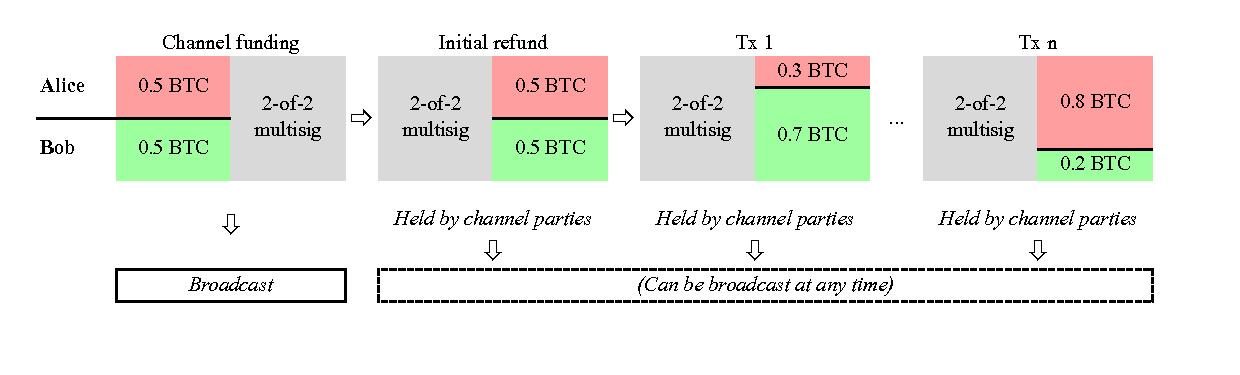
\includegraphics[width=0.9\linewidth]{channel_lifecycle.pdf}
\caption{Life Cycle of Payment Channel}
\label{fig:ChannelCycle}
\end{figure}

Whenever the parties decide to end there collaboration they can close the channel by broadcasting a closing transaction to the \gls{blockchain} which pays out each party its respective balance. While beneficial, collaborative channel closure is not required, each party can close the channel at any given time by broadcasting the latest transaction agreed upon. 

Participants in such channels are referred to as Lightning nodes, a computer system that runs an implementation of the Lightning Network protocol. Those nodes are not to be confused with Bitcoin nodes. However, since most Lightning nodes need direct access to the Bitcoin \gls{blockchain} most Lightning nodes are Bitcoin nodes at the same time.

\subsubsection{Using other Channels for Payments}
Since a payment channel is a biparty relationship any update of channel balance can only ever represent a transaction between those parties. Instead of opening a channel to each participant, a node wants to transact with there is the opportunity to route payments through multiple channels.

Economical transactions between two nodes often occur only once. It would, therefore, defeat the purpose of Lightning to open a channel for this unique payment because both the opening and closing of a channel takes each one transaction on the base \gls{blockchain}. Using Lightning would not use the load on-chain but rather increase it by a factor of two. This demonstrates that a payment channel should only be opened if the cost of doing so can be amortised over many transactions. This is either the case if the channel parties are expected to repeatedly transact with each other or if they can facilitate transactions between other nodes in the network through routing. 

Handling payments off-chain so far only worked between two parties that update Bitcoin transactions off-chain with the security of claiming their balance at any time on-chain. How can payments through multiple channels be accomplished without introducing trust into the system? If Alice wants to pay Carol through Bob, how can she be ensured that Bob will not keep the money and refuse to pay Carol? The solution are so-called \emph{Hash Time-Locked Contracts} or short \gls{htlc}.

First Alice asks the payee, Carol, to create and keep a secret $R$. This so-called \emph{\gls{preimage}} is hashed by Carol and the resulting \gls{hash} $hash(R)$ is shared with Alice. Alice then uses the \gls{hash}, to create a special \gls{htlc} transaction that promises Bob to receive the payment amount if he knows the preimage $R$. Bob also gets informed by Alice who is next in the path to find out this secret. Bob then himself creates an \gls{htlc} with the same preimage to Carol offering her the same amount upon disclosure of $R$. Carol is the payee in the transaction and has knowledge of $R$ so she could technically claim the funds on-chain. There is however an easier solution than this. After she releases $R$, Carol and Bob can simply agree to update their channel to reflect this payment. The same is done between Alice and Bob leading to the state where all channel balances are updated and the \gls{htlc}s is rendered useless. This mechanism is called ``time-locked'' because the offer of payment to the knowing $R$ is only valid for a certain timespan. If $R$ does not get released until the defined expiry the \gls{htlc} turns invalid. Therefore, each successive \gls{htlc} must have a lower timespan.

\subsubsection{Routing}\label{subsec:routing}
The previous chapter explained how a payment can utilize multiple channels to reach its destination without the introduction of trust between participants. This section describes how routing takes place and what trade-off needs to be made.

To ensure the privacy of payments the routing protocol uses \emph{\gls{onionrouting}}. The sender of the payment encrypts the information in multiple layers so that each hop only learns about the next hop in the path. Each intermediary node only knows where the payment comes from and where it goes next. The identity of the payer and the payee remain secret. Only the last node in the path finds out that it is the actual receiver of a payment.

\begin{figure}[H]
\centering
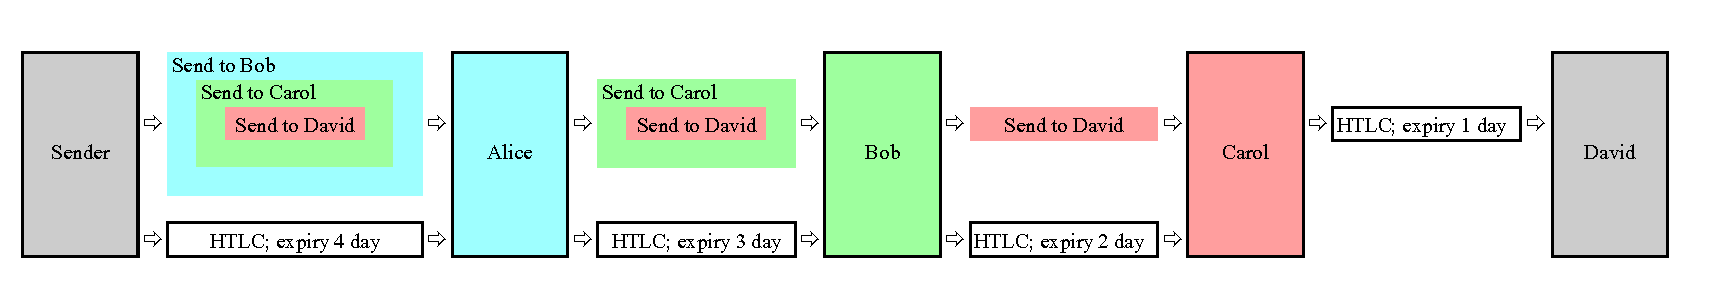
\includegraphics[width=1.0\linewidth]{htlc.pdf}
\caption{Onion Routing Schema}
\label{fig:onion}
\end{figure}

Figure~\ref{fig:onion} color codes the information which is only readable by the respective node with the same color. In each step, the outermost layer is decrypted and the next hop gets revealed. The remaining encrypted data is passed on down the line. This ensures that each node only has a local view of the path, knowing only about its predecessor and successor. Thus follows, the source of the payment needs to determine the complete path before sending payment.

Sending a payment requires the sender to find a viable path to the recipient. This is called \emph{\gls{sourcerouting}} and necessitates some information about the channel graph. When a new channel opens the parties notify the network about the channel, its capacity, and the fee policies. Each other network participant stores this information and builds up its local view of the network. When a node constructs a payment it can query a path with enough capacity along all its channels, though this is not enough to be certain that the payment can be routed. The payment in Figure~\ref{fig:nopayment} of $0.5$ BTC can not be routed from Bob to Carol as Bob only owns $0.2$ BTC of the $1$ BTC channel between him and Carol. This information however is only known to Bob and Carol, not to Alice. Alice only sees the public information which tells her that the channel has 1 BTC capacity. Local channel balances are kept private for two reasons. Every payment over a channel makes its balances to move. Keeping all nodes updated about all channel balances would necessitate to update them about every transaction. This is exactly how Bitcoin on the \emph{\gls{base}} works and the reason it does not scale. Secondly, informing the Network about every transaction is very bad for privacy, as an observer could easily determine who pays to whom over what path.

Not knowing the local balance distribution of channels makes it hard for source nodes to construct a reliable path. When a payment fails along the path a new route can be calculated and tried. This however is coupled with time delays that can cause a negative user experience.

\begin{figure}[H]
\centering
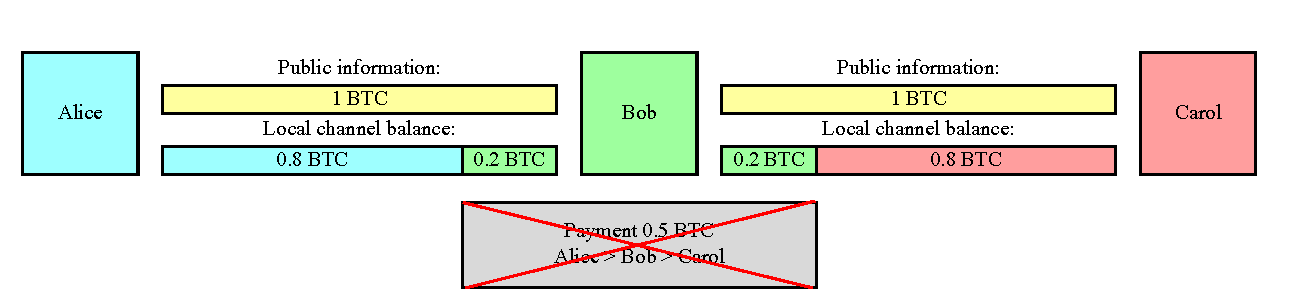
\includegraphics[width=1.0\linewidth]{nopayment.pdf}
\caption{Failed Payment Because of Insufficient Channel Balance}
\label{fig:nopayment}
\end{figure}

\subsubsection{Currency Units}\label{subsub:units}
Analogous to national currencies in which one unit is often divided into a hundred smaller subunits also one bitcoin can be divided into smaller elements. The Bitcoin block chain operates with the smallest unit called \emph{satoshi} or short \emph{sat}. This is $\frac{1}{100'000'000}$ of one bitcoin. Although named after the \gls{pseudonymous} founder it should not be confused with it. From now on satoshi refers to the unit. 

Any value smaller than one \emph{sat} can not be recorded on the block chain. However, when transacting within the Lightning Network not all transactions need to be settled on the base chain which allows for even smaller sub-units. One \emph{millisatoshi} or short \emph{msat} is one-thousandth of one satoshi. While other units are common in specific applications Table~\ref{tab:units} lists the units which are used in this work.

\begin{table}[H]
\centering
\begin{tabular}{l l S l} 
  {Unit} & {Abbrevation} & {Decimal (BTC)} & {Usage}\\ \hline 
  {bitcoin} & {BTC} & 1.0 & {Base unit; most popular}\\  
  {satoshi} & {sat} & 0.00000001 & {Native to the base layer}\\ 
  {millisatoshi} & {msat} & 0.00000000001 & {Native to the Lightning Network}\\ 
\end{tabular}
\caption{Bitcoin Currency Units Used in this Thesis}
\label{tab:units}
\end{table}

\subsection{Previous Work}
The research published by \textcite{pickhardt_imbalance_2019} serves as a base to formulate the question for this thesis. In their work, they present a solution for the pathfinding problem in a privacy-aware payment channel network. The proposed solution includes a rebalancing protocol which the nodes of the network should follow to achieve a higher balancedness for both itself and the entire network. It consists of instructions to proactively rebalance their channels within their friend of a friend's network, redistributing the relative funds owned in a channel but leaving total funds owned unchanged.

Rebalancing is an activity where one node engages in a circular payment that pays itself (see also Section~\ref{subsec:rebalancing}). This is only possible when the node has at least two channels with different peers. The payment gets routed \emph{out} through one channel and is \emph{received back} over another. On the way, it can use one or more hops to find back to the sender node. This procedure enables a node to change the balances of the individual channels while the total node balance stays the same. In practice, there would be a fee collected by the intermediate nodes whose channels are used. In the proposed rebalancing protocol nodes would forego the fee and only participate in the rebalancing attempt if their balancedness improves as well. The rebalancing algorithm is described in more detail in Section~\ref{subsec:rebal_algo}. 


\subsection{Problem Statement}
These payment channel networks are decentralised by nature and protocol changes can not be forced upon the node operators. Therefore, the question arises on how effective this protocol change will be assuming only partial participation of nodes. What are the effects of different levels of participation on the imbalance measure\footnote{defined as the inequality of the distribution of a nodes channel balance coefficients} of the network during repeated rebalancing cycles? What is the effect of different levels of participation on the network's ability to route payments between random nodes? 

In the next section, some fundamental graph theory concepts are formally introduced. An overview of some general graph theory problems is briefly elaborated. The field of problems is then narrowed down to the ones that find application in this thesis.

Section~\ref{sec:rebal} elaborates on the rebalancing algorithm proposed in a protocol change. Section~\ref{sec:experiment} lays out what experiments are conducted and how improvement is measured while Section~\ref{sec:method} goes more in-depth about the implementation. Results are presented in Section~\ref{sec:result}. Finally, Section~\ref{sec:concl} summarises the findings and gives some clues about possible future research.

\newpage
\section{Graph Theory Concepts}\label{sec:graph}
Graph theory is an old discipline that can be used to solve multifaceted problems in the real world. The following chapter contains an introduction to the basic principles and terminologies. It then defines different problems for which graph theory can be applied to find solutions. More emphasis is given to the topics which apply to the Lightning Network.

\subsection{Formal Definition}\label{subsec:formal}
The following paragraph defines the fundamentals of graph theory as described by \citet{rosen_discrete_2012}.
A graph $G=(V,E)$ consists of a set of vertices $V$ and edges $E$. An edge consists of two vertices which are called its endpoints. In an undirected graph, the endpoints are unordered, whereas the pair of vertices in a directed graph is ordered. The edge $(u, v)$ of a directed graph starts at $u$ and ends in $v$. In a \emph{simple directed} graph each directed edge can appear only once. When multiple edges go from one start vertex to the same end vertex the graph is named \emph{directed multigraph}. An edge that connects a vertex to itself is called a loop. Assigning weights to edges allows for more complex representations of mere connection and is useful if the real-world representation of a connection has certain \emph{cost} or \emph{distance} that one might want to minimise (maximise). 

The \emph{diameter} of a graph defines the longest distance between any two vertices. In other words, it is the longest of all shortest paths. In case the graph has weighted edges, those have to be considered for determining the shortest path.

Some vertices are better connected to the rest of the graph than others i.e. having a higher edge count. This edge count is referred to as \emph{degree} of a node. In a directed graph the in-degree (edges pointing towards a vertex) and out-degree (edges pointing away from a vertex) can be distinguished. 

A graph is called \emph{planar} if it can be drawn on a plane without any edges intersecting. However, some drawings show crossing edges, there might be a planer representation. E.g. Figure~\ref{fig:planar} shows two representations of the same graph. Since there is a planer representation, it is a planar graph. 

\begin{figure}[H]
\centering
\includegraphics[width=0.6\linewidth]{planar.png}
\caption{A Non-Planar and Planar Representations of the Same Graph, from \cite{rosen_discrete_2012}}
\label{fig:planar}
\end{figure}

The cut of network $G=(V,E)$ is a partition of $V$ into two disjoint subsets $S$ and $T$. The cut is determined by a set of edges which each have one endpoint in $S$ and another in $T$ \citep{brossard_graph_2010}. In Section~\ref{subsubsec:maxflow} the cut is used to determine the minimum cut that minimises the capacity of the cut in a flow network.

\subsection{General Problems}\label{subsec:genprob}
The beginning of this section explores the large field of problems within the discipline of graph theory. The specific field of network flow is then examined in greater depth. Eventually, the formally defined problem is applied to the Lightning Network and the thesis question.

\subsubsection{Graph Coloring Problems}
In \emph{graph colouring problems}, vertices represent areas on a map. Areas that share a border are connected with an edge. The goal is to use as little colours as possible to colour each area/vertex in such a way that adjacent areas have different colours. This minimum number is called the \emph{chromatic number} $\chi(G)$. \textcite{steen_four-color_1978} have delivered the proof to what was assumed to be true for a long time already; the chromatic number of a \emph{planar graph} is never greater than 4. 

Graph colouring finds many applications in planning and scheduling tasks. When scheduling final exams time slots have to be defined for different subjects so that no student has two exams at the same time. In a graph where vertices are the subjects and an edge between to subjects represent a common student, the resulting colours are the time slots.

\subsubsection{Subgraph Problems}
Certain properties of graphs can only be proven if they are fulfilled in all their \emph{subgraphs}. Hence, it is important to find those. A graph $H = (W, F)$ is a subgraph of $G = (V, E)$ when $W \subseteq V$ and $F \subseteq E$. A subgraph can be \emph{induced} by $W \subseteq V$ which means the edge set $F$ contains only edges of $E$ for which both endpoints are contained in $W$. Similarly the union can be built of two graphs $G_1$ and $G_2$ where $G = G_1 \cup G_2$ and $V = V_1 \cup V_2$. 

\subsubsection{Isomorphism Problems}
Another area of graph theory aims to determine whether two graphs are \emph{isomorphic}. This means \textquote[{\cite{rosen_discrete_2012}}, p. 668]{there is a one-to-one correspondence between their vertex sets that preserves edges}. Figure~\ref{fig:iso} demonstrates two structurally equivalent graphs. Although the vertex labels and the arrangement is changed, all pair of adjacent vertices in graph $G$ can also be found in $H$. 

\begin{figure}[H]
\centering
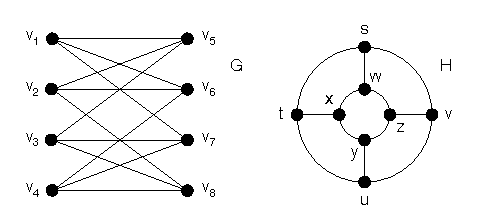
\includegraphics[width=0.6\linewidth]{isomorphism.pdf}
\caption{Two Structurally Equivalent Graphs, from \cite{gross_graph_2019}}
\label{fig:iso}
\end{figure}

Different algorithms exist that can determine isomorphism of two graphs, however with exponential worst-case time complexity. These algorithms mainly find application in chemistry and bioinformatics. Also, an example in integrated circuits can be thought of as described by \textcite{gross_graph_2019}. A computer chip company A develops a new efficient chip. Shortly after the launch, competitor B comes up with a very similar product. Suppose company A can prove an identical arrangement of circuitry on the board, they would have a case for a patent-infringement suit. They can apply algorithms to figure out whether there is isomorphism in the circuitries.

\subsubsection{Path Problems}
Different \emph{route problems} exist where the solution tries to find a path with certain properties within the graph. In the \emph{Seven Bridges of Königsberg}, in Figure~\ref{fig:konig}, the four sections of land are separated by a river and seven bridges are connecting them. The problem of passing every bridge exactly once and returning to the start can be formulated in terms of a graph with sections as vertices and bridges as edges. It is the question of whether a graph has an Euler circuit or not. 

\begin{figure}[H]
\centering
\includegraphics[width=0.6\linewidth]{koenigsberg.png}
\caption{Seven Bridges of Königsberg, from \cite{rosen_discrete_2012}}
\label{fig:konig}
\end{figure}

Many real-world applications exist where each edge needs to be visited once. E.g. a post office worker that has to deliver mail on different roads would be interested to only visit each street once. Similarly, a machine that cleans the aisles in a grocery store can be programmed to find an Euler circuit that cleans each aisle exactly once.

\subsubsection{Shortest Path}
When edges have a weight assigned different problems can be modelled and optimised by finding the shortest path. A famous algorithm to find such a path is \emph{Dijkstra’s algorithm}. According to \textcite{gross_graph_2019} Dijkstra's algorithm is a tree-growing algorithm. This means it starts with a given vertex and grows in a tree-like structure only one edge in each step. Consequently, the algorithm produces an entire tree of shortest paths to all other nodes in the graph. Dijkstra’s algorithm only guarantees to find the shortest path as long as all the edge weights are non-negative. In graphs with negative weights, Floyd’s algorithm can be used alternatively.

Similarly, in the Traveling Salesperson Problem, each vertex needs to be visited exactly once before returning to the starting point. Algorithms finding a path with low cost often use heuristics since no algorithm with polynomial worst-case complexity exists. Using heuristics in an algorithm means that one uses a guideline to make a decision instead of exhausting all possible options. While sacrificing the guarantee to find the best solution it is often the only way to solve the problem within a reasonable amount of time.

\subsubsection{Network Flow}
Different problems deal with the \emph{flow} in a network. Such networks have a capacity assigned to each directed edge. Often the goal is to find the maximum flow between a source and a sink node such that all intermediary nodes have equal in and outflow \citep{even_network_1975}. The next section explains more about this field of graph theory as it is most related to the problem encountered in the Lightning Network.

\subsection{Network Flow}\label{subsec:flow}
Payments in the Lightning Network can be described by a flow network as was introduced at the end of the previous chapter. This section explains the principles of such networks in more detail based on the definitions by \cite{wilson_introduction_2010}.

Many real-world problems deal with transporting something over a network with limited capacity. A simple example would be a logistic company that has to ship goods from a production site to an inventory. A train network provides multiple connections between the two locations via other intermediate stations. Each connection has a limit on how many goods can be transported per period. The company would like to know the maximum it can transport from the source to the target in a given period. In Figure~\ref{fig:flow_graph} node $s$ represents the manufactury, node $t$ the inventory. The intermediate stations $v_i$ are connected and the number represents the capacity limit.

\begin{figure}[H]
\centering
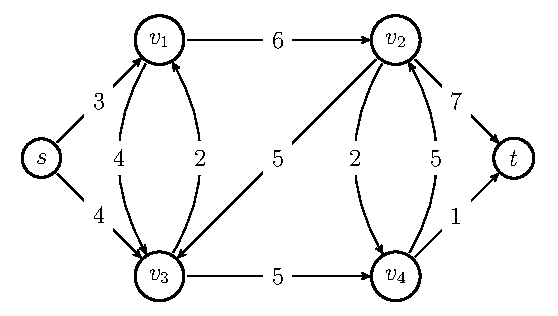
\includegraphics[width=0.6\linewidth]{flowgraph_1.pdf}
\caption{Flow Graph Annotated With Capacities, from \cite{brossard_graph_2010}}
\label{fig:flow_graph}
\end{figure}

From the above example the situation can be generalised by a \emph{weighted digraph} $G=(V,E)$ as defined by \cite{brossard_graph_2010}. The weight of an edge $e=(u,v)$ represents its \emph{capacity} $c(u,v)\geq0$. A vertex $v$ with an \emph{indegree} $indeg(v)=0$ is called source, and one with an \emph{outdegree} $outdeg(v)=0$ is called sink. Usually, it is assumed that there are only one source and one sink node. However, assuming the logistic company in the above example has multiple manufacturies and inventories, the problem can easily be reduced to this simple case. For any vertex $v \in V$ there is a path from source to sink that leads through $v$.

The \emph{flow} is defined by a function $f : V \times V \rightarrow \mathbb{R}$ which assigns a non-negative real number to all node pairs in the network. The following constraints must be satisfied
\begin{itemize}
  \item \textbf{Flow cannot exceed capacity}:
  $f(u,v) \leq c(u,v)$
  \item \textbf{Flows are symmetric}:
  $f(u,v) = -f(v,u)$
  \item \textbf{Flow must be conserved}: If $u \neq s$ and $u \neq t$, then $\displaystyle{\sum_{v \in V}f(u,v)}=0$
\end{itemize}

Those rules define that the flow between two nodes cannot exceed the assigned capacity. Each inflow into one node represents an outflow of the same amount from another. Each node (except for source and sink) must have equal inflow as outflow. Figure~\ref{fig:flow_graph_2} applies these rules to the previously discussed network.

\begin{figure}[H]
\centering
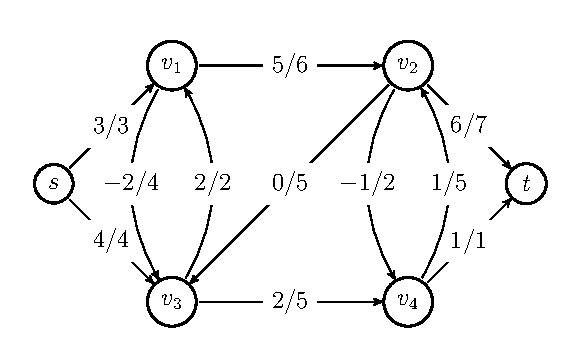
\includegraphics[width=0.6\linewidth]{flowgraph_2.pdf}
\caption{Flow Graph Annotated With Flow and Capacities, from \cite{brossard_graph_2010}}
\label{fig:flow_graph_2}
\end{figure}

The value of the total flow is denoted by $|f|=\displaystyle{\sum_{v \in V} f(s,v)}$, calculated as the sum all flows out of the source $s$. By definition, this is equal to the sum of inflows in the sink node $t$.

\subsubsection{Maximum Flow Problem}\label{subsubsec:maxflow}
As initially stated with the logistics example, flow networks are used to determine the maximum flow that can be transferred from source to sink. In other terms, one tries to find a flow function $f$ that maximises $|f|$. One example of such an algorithm is the \emph{Ford-Fulkerson} algorithm first introduced by \textcite{ford_maximal_1956}.

The algorithm start with the network and its capacities but no flow at all. It then start building up the flow step wise. In a temporary variable also the residual Network with the residual capacities are stored. The \emph{residual capacity} is the leftover capacity of an edge that is not yet used by the flow. For every edge $(u,v) \in E$ it is denoted as $c_f(u,v) = c(u,v)-f(u,v)$. Accordingly, the \emph{residual network} is defined as $G_f = (V, E_f)$, where $E_f=\{(u,v) | u, v \in  E \land c_f(u,v)>0\}$.

In a flow network $G = (V, E)$ with a source node $s$ a sink node $t$ the Ford-Fulkerson algorithm maximises the total flow $|f|$ as follows:

\begin{enumerate}
  \item For each edge $(u,v) \in E$, initialize $f(u, v)=f(v, u) = 0$
  \item If there is a path $P$ from $s$ to $t$ in the residual network $G_f$, continue to step 3, otherwise terminate.
  \item Set $c_f(P) = \min\limits_{(u,v) \in P} c_f(u, v)$.
  \item For each $(u,v) \in P$, set $f(u,v) = f(u, v) + c_f(P)$ and $f(v,u) = -f(u,v)$.
  \item Return to step 2.
\end{enumerate}

Effectively, the algorithm iterates over all paths from $s$ to $t$ in the residual network and add the capacities to the flow function. When there is no more path in $G_f$ connecting $s$ and $t$ this means the minimum cut (min-cut) is found. This is the cut with the minimum possible capacities of all cuts. \textcite{ford_maximal_1956} have shown that this min-cut is equivalent to the maximum flow. 

\subsection{Application in the Lightning Network}
The Lightning Network can best be described by an \emph{attributed simple directed graph}. That is a graph with directed edges without loops and multiple directed edges. Since a payment channel between $u$ and $v$ allows payments to flow in both direction it can be modelled by use of two edges $(u, v)$ and $(v, u)$. Two edges are needed to model local balances and fees as \emph{attributes} since they differ in the two directions.

In terms of network flow theory (see Section~\ref{subsec:flow}), the capacity $c(u,v)$ is defined as the local channel balance of node $u$. This represents the maximum amount that can be sent from $u$ to $v$. Figure~\ref{fig:channel_graph} visualises a channel between Alice and Bob with 1 BTC capacity of which Alice holds 0.2 BTC and Bob holds 0.8 BTC as local balances. 

\begin{figure}[H]
\centering
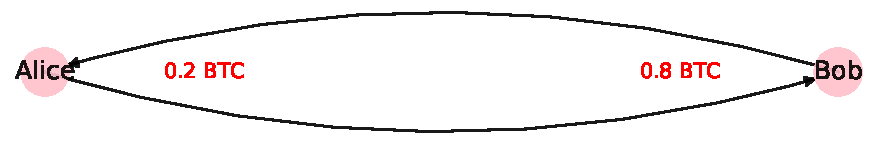
\includegraphics[width=0.9\linewidth]{simple_channel.pdf}
\caption{Lightning Channel Represented as Attributed Simple DiGraph}
\label{fig:channel_graph}
\end{figure}

\subsubsection{Fees}
As mentioned earlier, the Lightning Network allows nodes to use other payment channels to find a path to the recipient. Since this activity involves the utilization of foreign capital, nodes can charge a fee. This can be compared to a toll that needs to be paid by everyone crossing the bridge. The fee consists of two parts, a fixed fee and a variable fee. While the fixed fee is the same for every payment, the variable increases linearly with the amount being transferred. Those fees can be applied to graph theory concepts as a weight. Hence, whenever finding the shortest path in the Lightning Network, this results in finding the cheapest path.

\subsubsection{Path Finding Problem}\label{subsubsec:pproblem}
As laid out in Section~\ref{subsec:routing} the initiator of payment needs to construct the path before sending the payment. Nodes trying to find such a path work with limited information. While they know what channels are available and what their capacities are, they do not know about the balances and therefore whether the nodes can forward their payment or not. Hence, it is likely that a payment attempt fails because a node had insufficient balance. The paying node needs to find another route and retry the payment until it succeeds. If the payment fails repeatedly it can cause delays that incur a bad user experience.

This problem gets amplified because in the current protocol channels are single funded. This means one party provides 100\% of the channel capacity. A collaborative approach to funding a channel might be possible in the future. As a consequence, the funder of the channel owns initially 100\% of the channel balance and the other side 0\% which means the channel can only be used to route into \emph{one direction}. A third party trying to route through this channel has a 50:50 chance that he or she can not even route a minimal amount of 1 sat. 

One can think of this path finding problem as a flow network (see Section~\ref{subsec:flow}) where the capacities are not entirely known. More precisely, for a payment channel between $u$ and $v$, the summed capacity $c_{sum} = c(u,v) + c(v,u)$ is known. However the value for the individual capacities can be $c(v,u) = [0, c_{sum}]$. Hence, nodes only know the upper limit for a capacity. 

Routing in the Lightning Network deviates from flow networks in another aspect. The flow, as previously described, is the total amount that can be transferred using all paths between the source and the sink. In the current Lightning Network \emph{single path payments} are the standard. This means a payment uses only one path. This limitation is due to the nature of how \glspl{htlc} are constructed. \glspl{htlc} ensure atomicity by building a path that either succeeds or fails. So, no intermediate node is paid, when the receiving node is not paid. While multiple subsequent single path payments could be sent, there is a risk that some of them would arrive and others not. A solution to this limitation is being developed at the time of writing. \emph{Atomic Multipath Payments} (AMP) will allow the utilisation of multiple paths in one atomic payment. This new method has the obvious advantage that the payment amount is no longer limited to the largest capacity but can be split and sent over multiple payment channels. On the other hand, there are also some disadvantages when not all paths succeed within a reasonable time limit. E.g. 2 out of 3 paths succeed, but for the entire payment to settle the last path is needed. Until then the successful two paths are blocked and need to wait. Since AMP is not yet widely adopted this thesis focuses on single path payments only.

Section~\ref{subsubsec:pproblem} explained why finding a payment path is difficult in the Lightning Network. Since the capacity that can be sent over a payment channel can be anything between 0 and the total channel capacity, nodes can only guess how the balance is distributed and how much actually can be forwarded. 

Generally, for routing it is a disadvantage when a channel's capacity is allocated completely on one side since this means it can only route in one direction. Hence, it can be concluded that a more balanced allocation of funds is desirable and allows more options to route payments.

To achieve a more balanced network was the goal of \textcite{pickhardt_imbalance_2019} when they proposed a mechanism in which nodes proactively work towards better balance. Employing rebalancing, nodes would constantly reallocate the balances of their channels, trying to achieve an optimum balance. The reason why nodes do not do this already is the fees that need to be paid. Therefore, they proposed a fee-free rebalancing protocol which is described in more detail in Section~\ref{sec:rebal}.

\subsubsection{Partial Participation}
In an empirical simulation, \citeauthor{pickhardt_imbalance_2019} showed how the ability to route payments would improve if the protocol would be adopted by all nodes. 

Similar to the Bitcoin network also the Lightning Network is a decentralised network without any central control. This means all participants are free to join and leave, as well as to decide what software implementation they run. Therefore, it is not possible to upgrade all participating nodes at once. Each node would adopt this new protocol individually and some might decide to not adapt at all. 

The main question arises, how effective the proposed protocol change is under partial participation and what influence have different adoption scenarios. Simulations are utilised to find answers to these questions.

In the next sections terminology native to the Lightning protocol is used. A directed graph is referred to as the \emph{network}. Vertices are called \emph{nodes} and a pair of opposite directed edges are a \emph{channel}. The \emph{channel capacity} defines the total amount of bitcoin locked in a channel and is distributed between the two node's local balances. The amount which can be sent by a node over one of his channels is defined by the node's \emph{balance}. The terms \emph{route} or \emph{path} are used interchangeably and are defined by a set of channels that can be traversed. \emph{Fees} is the general term that includes both \emph{fixed fees} and \emph{variable fees}. \emph{Rebalancing} is the activity of routing a payment in a circle back to the initiating node and is used to reallocate balances within the set of channels a node controls.   

\newpage
\section{Proactive Rebalancing Protocol}\label{sec:rebal}
\textcite{pickhardt_imbalance_2019} proposed in their paper a rebalancing algorithm which when proactively executed would improve the overall networks ability to route payments. The next sections define the algorithm in more detail and formally defines the protocol change. In Section~\ref{subsec:sim_rebal} the implementation is shown in greater detail.

\subsection{Rebalancing}\label{subsec:rebalancing}
Figure~\ref{fig:rebal} shows an example network with four nodes and four channels that were recently opened. The capacities are hence all on one side of the channel. Such an allocation of balances limits the use of the channels severely as they can only forward payments into one direction. If Alice wants to have a better balance among her channels she can start a process called \emph{rebalancing}. This is a self-payment which routes an amount from one of her channels through the Lightning network to another of her channels. In this example, Alice decides she has excess balance in the channel with Bob and insufficient balance in the one with David.

\begin{figure}[H]
\centering
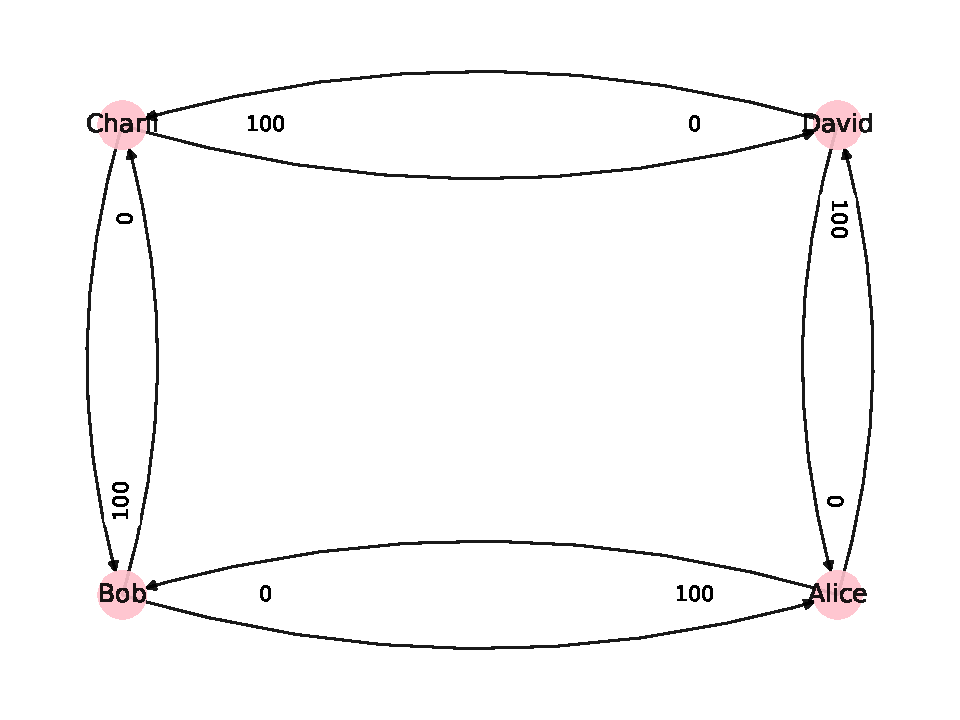
\includegraphics[width=0.9\linewidth]{rebalancing.pdf}
\caption{Initial State of Newly Opened Channels}
\label{fig:rebal}
\end{figure}

She can now construct a payment of e.g. 40 with the path [Alice, Bob, Charli, David, Alice]. This reduces her balance in the channel with Bob by 40 (new 60) and increases her balance in the channel with David by 40 (new 40). Both of her channels are now better balanced and allow for more payments to be routed. The resulting state is shown in Figure~\ref{fig:rebal2} and the path of the rebalancing payment is indicated in red. 

This action performed by Alice did of course not only change the balances of the channels she is involved but also the ones she used to route the self-payment. In this case, the channels between Bob-Charli as well as Charli-David are also more balanced. While this was the case in this example it is not guaranteed to be true in all cases, it might well be that some channels end up less balanced. The reason why all the nodes are incentivised to participate are fees that they can collect on each payment they forward. They do not even know that this payment is a rebalancing transaction. Hence, Alice has to pay fees for this rebalancing operation. 


Rebalancing can be summarised as an activity performed by a single node attempting to improve the local balances of its channels by sending a payment out through one channel with excess balance and receiving it through a channel with too little balance, effectively paying itself. For all the nodes in the routing path, this payment looks no different from any other payment, so they charge their normal routing fees. While the balances within the channel change a node's total balance remains constant. Alice still has a total balance of 100 allocated differently among her two channels. 

\begin{figure}[H]
\centering
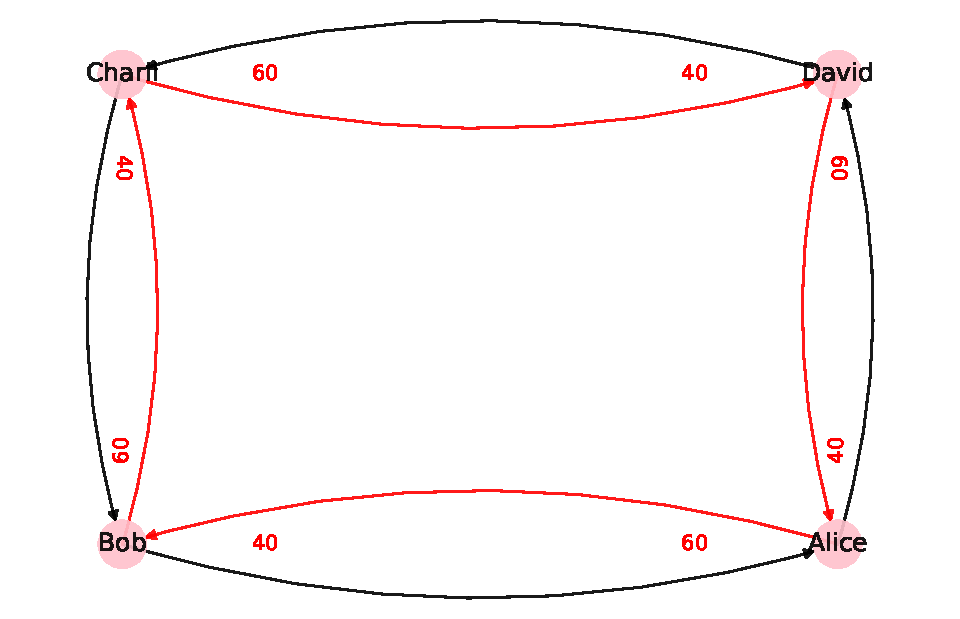
\includegraphics[width=0.9\linewidth]{rebalancing2.pdf}
\caption{Rebalancing from Alice through Bob, Charli and David}
\label{fig:rebal2}
\end{figure}

\subsection{Rebalancing Algorithm}\label{subsec:rebal_algo}
The previous section was about how nodes can \emph{improve} their channel balances. While the improvement in the example was quite clear it has to be stated what the ultimate goal is towards which the nodes try to improve. Intuitively, a distribution of 50:50 in each channel could be thought of as an appropriate goal. In reality, this is not a feasible target as the next section will show.

\subsubsection{Imbalance Definition}
The following terms will first be defined to better understand the problem. The two nodes in a payment channel $e=(u,v)$ are denoted as $e_u$ and $e_v$. The capacity of $e=(u,v)$ is privately split among the two nodes channel balance $b(e_u)$ and $b(e_v)$. Therefore, the capacity of the channel $c(e)=b(e_u)+b(e_v)$. The \emph{channel balance coefficient } for $u$ represents the ratio node $u$ has in a channel $e=(u,v)$ and is defined as $\zeta{(u,v)}=\frac{b(e_u)}{c(e)}$. Respectively, for the node $v$ the coefficient is $\zeta{(v,u)}=\frac{b(e_v)}{c(e)}$. As both balances make up the total capacity it follows  $\zeta{(u,v)} + \zeta{(v,u)}=1$. Let us define all the channels node $u$ is part of as $U=n(u)$. The \emph{total funds} the node $u$ owns can be denoted by $\tau_u:=\displaystyle{\sum_{e\in U}b(e_u)}$. The \emph{total capacity} of the node's channel $\kappa_u:=\displaystyle{\sum_{e\in U}c(e)}$. We can now define the \emph{node balance coefficient} as $\nu_u = \frac{\tau_u}{\kappa_u}$.

Both $\tau_u$ and $\kappa_u$ must remain constant during rebalancing operations. This is because the rebalancing payment pays always the node itself, so the \emph{total funds} of a node can not increase or decrease. As no new channels are opened or closed and capacities in the existing channel can not be changed \emph{total capacity} must remain constant. The initially stated goal to have a 50:50 distribution in all channels is only achievable with a \emph{node balance coefficient} of $0.5$. As this coefficient remains constant only nodes that already have a node balance coefficient of $0.5$ could reach that state.

\citeauthor{pickhardt_imbalance_2019} had to come up with a different balance measure which applies to all nodes no matter what node balance coefficient they had. So they generalised the rule discussed in the previous chapter. Every channel of node $u$ should have the same \emph{balance coefficient} $\zeta{(u,v)}$ which would then equal the \emph{node balance coefficient} $\nu_u$. In other words, making all channel balance coefficients as similar as possible. They then defined a measure to assess how well this is achieved for a particular node. The \emph{\gls{gini}} coefficient measures the inequality of a distribution. For a node $u$ with channel balance coefficients $\zeta_{(u,v_1)},\dots,\zeta_{(u,v_d)}$ they define

$$G_u = \frac{\displaystyle{\sum_{i\in U} \sum_{j \in U}} | \zeta_i - \zeta_j |}{2 \displaystyle{\sum_{i \in U} \sum_{j \in U} \zeta_j}}$$

When all balance coefficients are equal the \gls{gini} coefficient $G_u$ turns to $0$. A value of $G_u=1$ represents the most unequal distribution \citep{pickhardt_imbalance_2019}.

Figure~\ref{fig:gini_example} shows an initial channel state with various balance coefficients. The resulting \gls{gini} score is $G_u=0.3519$. With several rebalancing operations, this node can achieve a final state where all channels show the same relative distribution. Such a constellation has a \gls{gini} score of $G_u=0.0$. 

This example shows that this node could not have achieved distribution of 50:50 on all channels, since the node balance coefficient $\nu_u = 0.6$. However, making all channel balance coefficients $\zeta{(u,v_i)}$ equal to $\nu_u$ is an achievable goal for all nodes. 

\begin{figure}[H]
\centering
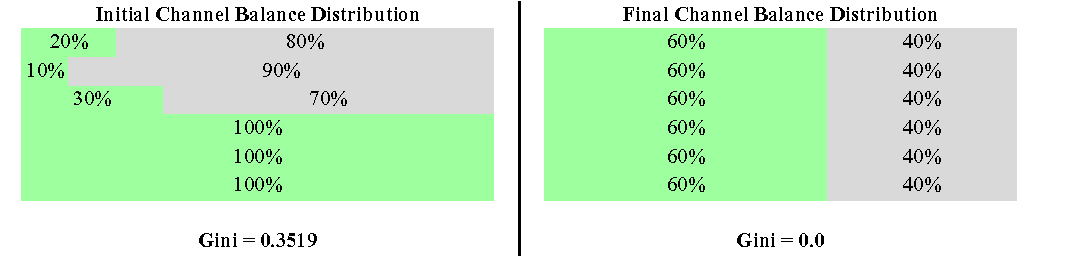
\includegraphics[width=0.9\linewidth]{gini_example.pdf}
\caption{Example of Two Distributions of Channel Balances and Their \gls{gini}s}
\label{fig:gini_example}
\end{figure}


\subsubsection{Proposed Algorithm}\label{subsec:prop_algo}
The proposed algorithm should be executed by each node individually. The main goal of each node is to achieve a low value of imbalance $G_u$. The node can improve its imbalance by repeatedly executing the following steps according to \cite{pickhardt_imbalance_2019}:

\begin{enumerate}
\item A node $u$ computes its node balance coefficient $\nu_u$.
\item $u$ then computes its channel balance coefficients $\zeta_{(u,v_1)},\dots,\zeta_{(u,v_d)}$.
\item All channels $e=(u,v_i)$ for which the channel balance coefficient is higher 
than its node balance coefficient, are selected as $C = \{(u,v_i) | \zeta_{(u,v_i)} - \nu_u\ > 0\}$.
\item From the candidate set $C$ a random channel $e=(u,v)$ is selected.
\item Now the node searches for a circular payment to itself along $e=(u,v)$ by choosing a path $p = [v,x_1,\dots,x_n,u]$. The amount of that payment should decrease the value of $\zeta_{(u,v)}$ to that of $\nu_u$ and can be computed as $a = c(e)\cdot (\zeta_{(u,v)}-\nu_u)$. The end of the circle should be a channel $(x_n,u)$ for which the channel balance coefficient $\zeta_{(u,x_n)}$ is smaller than the node balance coefficient $\nu_u$.
\item The node conducts the payment if all the nodes on the path $p$ agree to participate. It could happen that some nodes will only participate with a value smaller than $a$. As this is already progress $u$ will accept the suggested amount instead of being stubborn. 
\item Repeat all steps as long as the local balance coefficients are not even enough and as long as paths are found.
\end{enumerate}

\subsection{Protocol Change}
Rebalancing itself is already supported in the current Lightning protocol as it includes normal payments where the sender and receiver are the same entity. However, the incentive to do so is very small. The initiating node is the one who pays the fee for the payment. A node would only do such transactions if it can expect to earn fees on the rebalanced channels that exceed the fees paid for the rebalancing. 

\textcite{pickhardt_imbalance_2019} propose a change in the protocol to make rebalancing more explicit. As the proposed algorithm in the previous Section~\ref{subsec:prop_algo} shows, only nodes would participate that also benefit from the rebalancing (step 6). As this would be a win-win situation for all participating nodes they could agree to forego the fees. This change towards a \emph{fee-free rebalancing} would incentivise nodes to do this proactively as soon as they see the opportunity to improve their balance.

Additionally, they recommend adopting a change in the communication protocol which allows \textquote[{\cite{pickhardt_imbalance_2019}}, p. 8]{the network to work collaboratively towards achieving a good balance by locally sharing rebalancing hints}. This sharing of local channel balances would only need to be done among the local neighbourhood of a node. This is where the nodes should look for rebalancing circles and providing hints advertises willingness to rebalance in a certain direction without revealing the exact balance of the channel in question. The privacy drawbacks are minimal as balances in the local neighbourhood can easily be probed anyways \citep{tikhomirov_probing_2020}. 
 
\subsubsection{Motivations to not Participate}
So far the presented algorithm sounded like a win-win situation for everyone and there would be no discussion around adopting it. However, it is not that simple. There are different reasons why nodes would not want to participate in such a change. Some nodes might not want to forego the revenues in fees. If they decide not to participate but most others do, they still benefit from the better overall balance of the network. So, without contribution, they can harvest the benefits of others who participate. 

\newpage
\section{Experiment}\label{sec:experiment}
Experiments are executed to find out how the effectiveness of proactive rebalancing is affected by different levels of participation. This section gives an abstract overview of what an experiment does, what parameters can be set and how it is executed. The subsequent Section~\ref{sec:method} explains the Python implemented in greater detail.

\subsection{Performance Measures}\label{sub:perfm}
The goal of rebalancing is to improve the overall networks ability to route payments between its nodes. The effectiveness of the algorithm can only be determined by measuring this ability with the help of \emph{performance measures}. This is the generic term for the measures defined in this chapter. Some of the presented indicators were previously defined and used by \textcite{pickhardt_evaluating_2020}. 

To make a statement about the entire network, all the presented measures consider the ability to route payments for every node in the network. As it is unclear what payments nodes would want to make, the best that can be measured is one payment between each node in the network. A network with $N$ nodes results in a complete payment graph with a total number of payments $N(N-1)$. The network from the experiments has 2139 nodes which result in 4'575'321 payments to test. This puts a limit on the computational complexity of the measures since expensive calculations become unfeasible on consumer hardware.

\subsubsection{Success Rate on Shortest Path}
The ability to conduct any payment between two nodes is very fundamental. This \emph{success rate} (\emph{\gls{sr}}) can be measured by attempting to send a minimal payment of 1 sat over all shortest paths between any two nodes. The fraction of paths which can accommodate the payment from all shortest paths is the \gls{sr}. As the evaluation of the \gls{sr} is done over and over again the list of all shortest paths is cached for later use. The function \mintinline{python}{networkx.all_pairs_dijkstra_path()} is used to retrieve them. The weight to calculate short paths is represented by the fee a node would need to pay. The fee is defined by a variable and a fixed fee. As payment sizes are not known for this calculation simply the base fee is used for the shortest path calculation. 

The \gls{sr} will give a good overview of how many nodes can reach each other with a minimal payment. The limitation of the measure is that it does not take payment size into account and minimal payments might not be very beneficial in reality.


\subsubsection{Payment Size on Shortest Path}
Similar to the \gls{sr} the \emph{median payment size} (\emph{\gls{mps}}) also considers the shortest paths between all node pairs. On all node pairs, the maximum amount that can be sent is calculated. This amount is defined by the smallest balance of edges along the path. From all possible payment amounts, the median is taken to come up with a measure for the entire network. Since the distribution of the payment amounts is expected to be highly skewed, the median is taken to summarise the data instead of the mean. This measure assesses how much the nodes can send to each other.

\subsubsection{Multi Path Retry}
Both \gls{mps} and \gls{sr} consider only the shortest path for their calculation. In reality, a node that receives a payment error would simply calculate new paths and retry the payment on those. A failed payment does not necessarily mean a bad user experience as several paths can be tried sequentially within a short amount of time. To account for this fact a measure will be defined that can check multiple paths instead of just one. The measure \emph{Multi Path Retry} (\emph{\gls{mpr}}) can be seen as a combination of the latter two. Additionally, the \gls{mpr} measure considers different payment sizes.

Between each node pair, not the shortest path is calculated but a set of 10 different paths. On each of those paths, three payments of different sizes are tried to be executed. A \emph{1 sat payment}, a \emph{micro payment} of 10'000 sat and a \emph{normal payment} of 100'000 sat. Each node pair then receives a score between 1 and 10 per payment size, depending on how many paths could route the payment. The median of all node pairs then gives an indication about the total network, considering different payment sizes and multiple paths.


\subsection{Simulating Proactive Rebalancing}\label{subsec:pro}
The main objective of the simulation is to see how the proactive rebalancing protocol described in Section~\ref{subsec:prop_algo} can be applied in the Lightning Network. To answer this, the simulation network resembles the real Lightning Network. Each experiment then executes the proposed rebalancing algorithm for each node in the network.

In reality, each node would execute the algorithm itself. However, since a simulation knows all nodes, channels and balances it is possible to calculate and execute the rebalancing in a holistic manner. Nevertheless, the limited information nodes have about the rest of the network must be respected. 

In a first step, cycles are being determined on which nodes would agree to rebalance. Such a rebalancing cycle can only be found if \emph{all nodes} want to rebalance in that direction. As the proposed protocol foresees to share hints about desired liquidity only in the local neighbourhood, the length of those cycles is limited. The local neighbourhood of a node is defined as the friend of a friend network. Let us assume node \texttt{self} in Figure~\ref{fig:foaf} has only two channels with \texttt{Friend1} and \texttt{Friend2}. These friends both provide information about all their channel balances (marked as green edges). This allows the node \texttt{self} to assess the path $p = [self, Friend1, D, Friend2, self]$ in regards to the node's willingness to rebalance. However, this restricts the paths for rebalancing to the ones of length 4 or 3. Although node \texttt{self} also knows about the channel $e = (C, X)$, it has no insight about their imbalance, since it is not part of the friend of a friend network. Hence, this path of length 5 is not considered for rebalancing.

\begin{figure}[H]
\centering
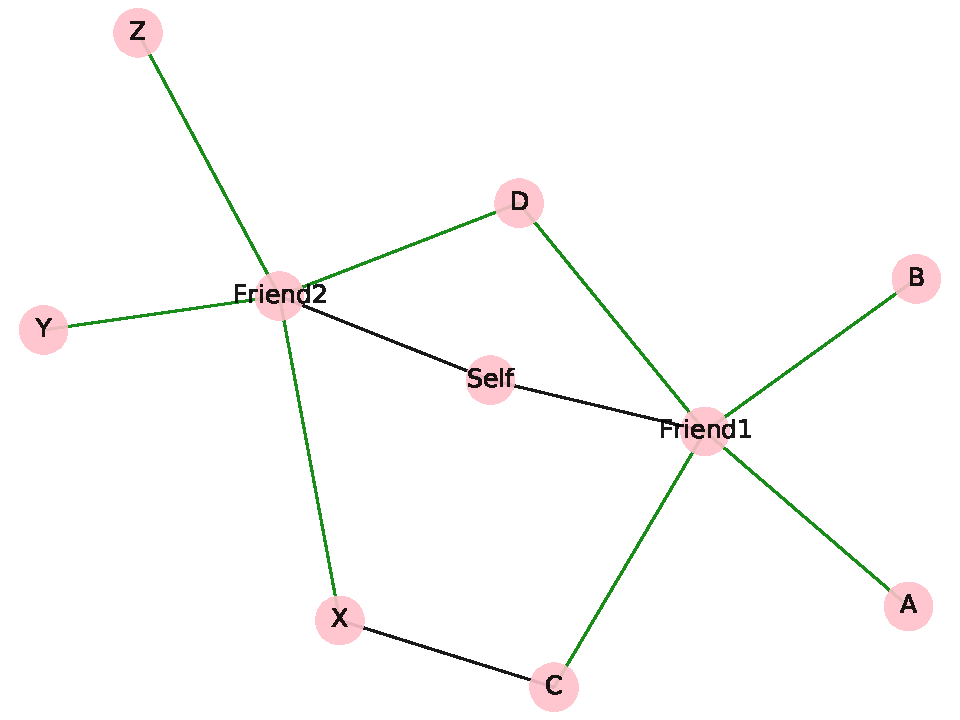
\includegraphics[width=0.9\linewidth]{foaf.pdf}
\caption{Sharing Rebalance Hints (Green) in the Friend of a Friend Network}
\label{fig:foaf}
\end{figure}

In the next step, rebalancing is executed within those cycles. For each payment, the maximum amount is found on which all participants agree. After each payment, the \gls{gini} score is calculated to record the progress towards a more balanced network. Similarly, performance measures are calculated. The rebalancing stops once there are no more circles on which at least one sat can be rebalanced. This simultaneously marks the end of the experiment.


\subsection{Selection Strategies}\label{subsec:selstrat}
While Section~\ref{subsec:pro} describes how proactive rebalancing is simulated it assumes that all nodes in the network participate. As the experiments aim to show the impact of different participation levels, the simulation has to be executed multiple times with different levels of participation. This is done since it can be assumed that not all nodes will adopt a new protocol immediately.

The network is heterogeneous in regards to the channel count and available capacity per node. The distribution of the payment channels appears to follow a power-law distribution. However, no test has been executed to prove this, since \textquote[\cite{clauset_power-law_2009}, p. 1]{the detection and characterization of power laws is complicated by the large fluctuations that occur in the tail of the distribution}. Figure~\ref{fig:channelcount}, however, shows that little nodes have a large number of channels and most of the nodes have only a few. The result of the experiment, therefore, will vary depending on how the participating nodes are selected. 

\begin{figure}[H]
\centering
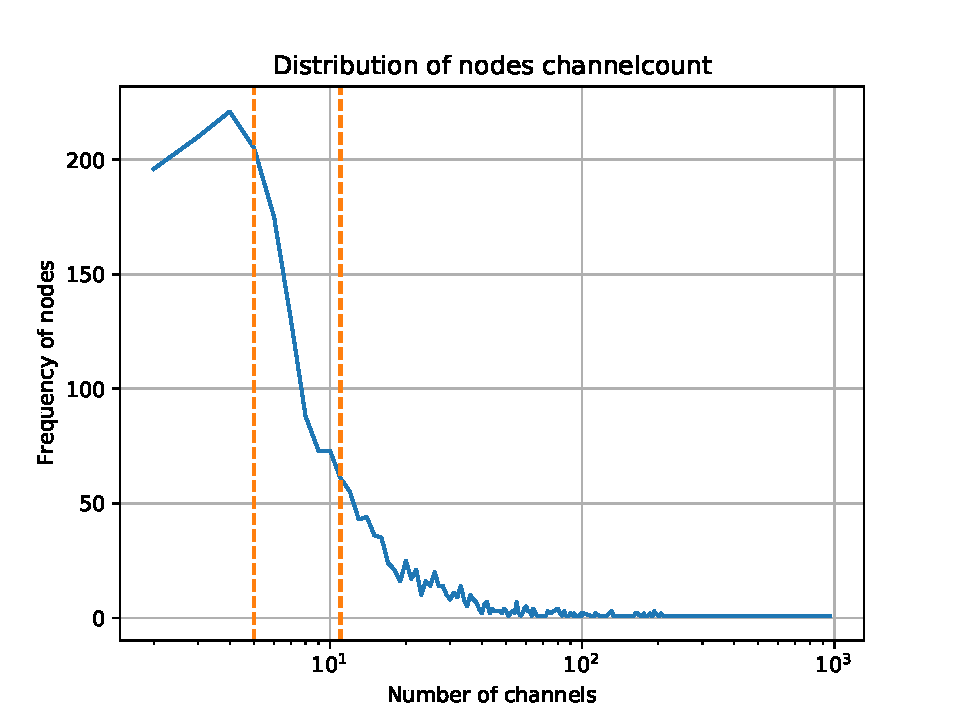
\includegraphics[width=0.7\linewidth]{channel_count_distr.pdf}
\caption{Frequency Distribution of the Node's Channel Count}
\label{fig:channelcount}
\end{figure}

\subsubsection{Randomised}
The randomised selection executes experiments with participation levels from 10\% to 100\% in 10\% intervals (10\%, 20\%, \ldots, 90\%, 100\%). The nodes are selected randomly. The set of nodes in a smaller participation level are a subset of the larger ones. To make the experiments reproducible the \mintinline{python}{random} package is seeded with a fixed value.

There is a disadvantage to this method. Multiple random selections with different randomness result in other results. It could be that by coincidence a disproportionate amount of either large or small nodes are selected. To reduce this effect the experiment runs 10 samples with different randomness and the average of the measures is calculated. 

\subsubsection{Node Ranking}
In another scenario, more important or less important nodes could decide to participate in the protocol change first. Such a selection strategy, hence, needs to sort the nodes by their importance in the network. This feature can be measured in multiple ways. This section shows some ways how the node's importance can be determined. A preliminary experiment will show whether there is a significant difference in the rankings obtained by the different methods.

The \emph{degree centrality} is a simple measure. It counts the degree, the number of edges connected to a node (see Section~\ref{subsec:formal}). The higher the value, the more central a node is \citep{golbeck_analyzing_2013}.

A slightly more sophisticated measure is the \emph{betweenness centrality}. It \textquote[\cite{golbeck_analyzing_2013}]{measures how important a node is to the shortest paths through the network}. A higher value means the node has an important location in the flow of information through the network. For the reason of simplicity, no special weights were used for the shortest path calculation. Which means each edge was weighted equally.

The \emph{eigenvector centrality} does not treat each neighbour equally. A node's importance will rise if it is surrounded by other important nodes. It can also be interpreted as a node's influence on the network \citep{golbeck_analyzing_2013}. A variation of eigenvector specialised for directed networks is \emph{pagerank}. Here, special weight is given to an \emph{in-degree} of an influential node. For the graph in this experiment, this does not make much sense, since all nodes connected with a payment channel are connected with two edges, one in each direction.

All these different methods return a score for each node by which one could make a ranking from least to most important. We want to proof the hypothesis that for the dataset at hand all rankings would be similar. In order to compare different rankings, a rank correlation can be calculated which measures the similarity of two rankings. Spearman's correlation is an appropriate way to test a monotonic relationship between two variables \citep{noauthor_spearmans_nodate}. It is not required for the distribution to be normal. The variables simply have to be on an ordinal scale. The resulting correlation coefficient is in the range $[-1,1]$ and is a measure for how strong the two rankings correlate. $0$ means no correlation while $1$ and $-1$ stand for a strong positive or negative correlation. Table \ref{tab:spearman} shows the result of the conducted experiment. All coefficients are fairly close together, therefore, these different ranking criteria all end up with a very similar ranking. From now on the degree centrality is used as a measure for importance since it is the simplest to calculate.

\begin{table}[H]
\centering
\begin{tabular}{c | cccc} 
{} & {Degree centr.} & {Betweenness centr.} & {Eigenvector centr.} & {Pagerank} \\ \hline 
{Degree centr.} & {1.0} & {0.845} & {0.916} & {0.988} \\ 
{Betweenness centr.} & {0.845} & {1.0} & {0.698} & {0.893}\\
{Eigenvector centr.} & {0.916} & {0.698} & {1.0} & {0.880} \\
{Pagerank} & {0.988} & {0.893} & {0.880} & {1.0} \\
\end{tabular}
\caption{Ranking Correlation Coefficients of Importance Measures}
\label{tab:spearman}
\end{table}

When simulating different level of participations the participating nodes can be chosen either from the top or the bottom of the ranked node list. This simulates an adoption starting by important or unimportant nodes respectively. 

\subsubsection{Node Categories}\label{subsub:categ}
Similar as in the previous experiment the degree centrality is taken as a measure for a node's importance. This ranked list is then split up in three categories. The boundaries between the groups are determined by \emph{equal frequency binning} to ensure equal-sized groups of 713 nodes in each group. Then participation levels from 10\% to 100\% are executed for each category individually. Hence, 100\% participation of one group corresponds to the participation of 33\% of the total network. 

Figure~\ref{fig:eqfreq} shows those boundaries in two different charts. Figure (a) is a cumulative histogram of the node degree (with a logarithmic scale). The boundaries fall on a node degree of 5 and 11. Figure (b) shows those same boundaries but with regards to how many channels those nodes contribute. It is visible that the number of channels is mainly concentrated in the last group. 

\begin{figure}[H]
\centering
\subfloat[Distribution of node degree]{
  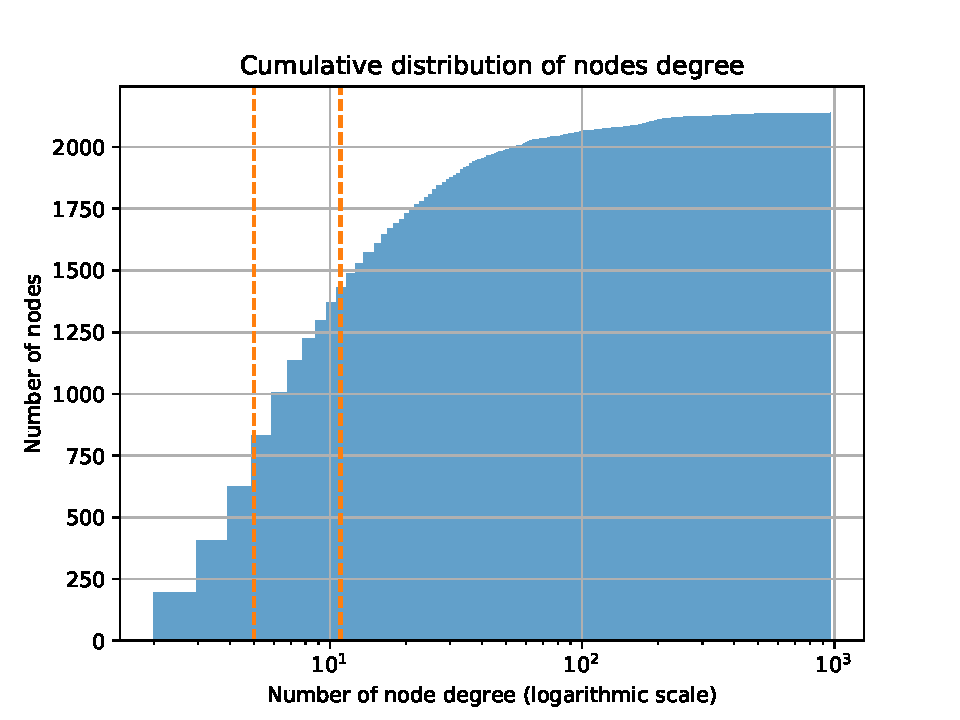
\includegraphics[width=0.45\linewidth]{cum_channel_distr_eq_width.pdf}
}\quad
\subfloat[Node's contribution to channels]{
  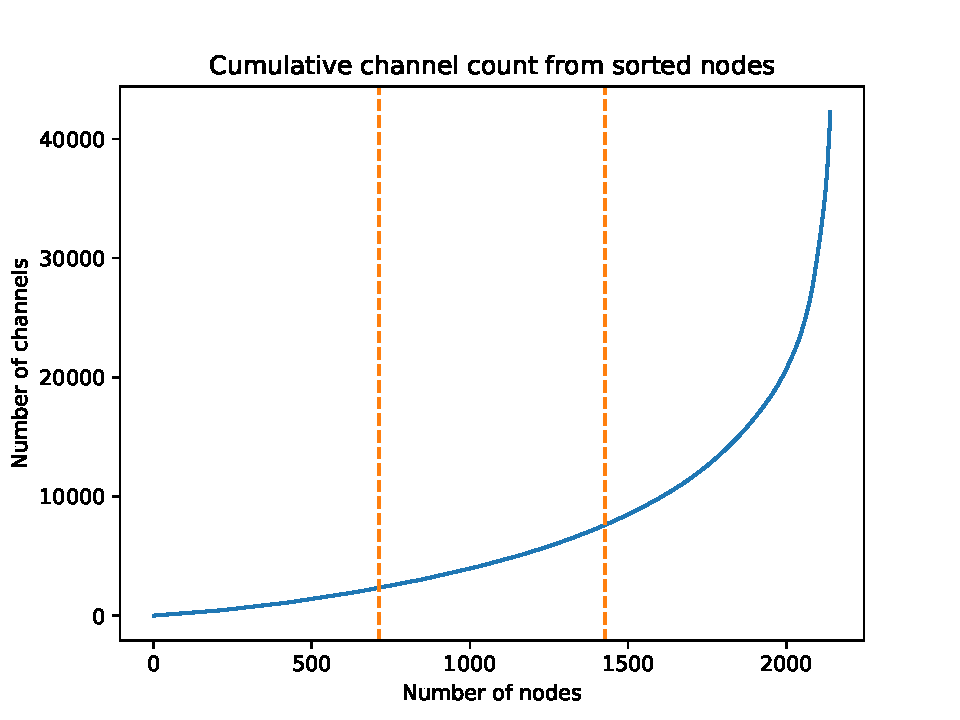
\includegraphics[width=0.45\linewidth]{node_count_to_contr_channel_count_eq_width.pdf}
}
\caption{Shows Boundary Definition by Equal Node Frequency}
\label{fig:eqfreq}
\end{figure}

\subsubsection{Network Spread}
For this node selection method let us assume that the adoption of the new protocol is being spread through the network. Nodes only start adopting it when someone in their neighbourhood has adopted it. The simulation, therefore, starts with an initial set of nodes which participate in round 1. In each iteration, a certain fraction of their channel partners participates as well. This results in \emph{two experiment parameters} which can be adjusted to simulate the way adoption takes place. 

\emph{Init parameter} defines how many nodes start adopting the protocol in iteration 1. \emph{Spread parameter} is the fraction of adjacent nodes that start participating after each iteration. Those two parameters should be chosen in a way that allows several participation levels similar to the 10 levels seen in the previous sections. Table~\ref{tab:param} shows the number of iterations required to reach either 99\% or 100\% of all nodes. The coloured columns and rows mark the parameters which were used for the experiments. An initial value of 2/10/15\% and a spread of 40/50/60\% result in total 9 experiments which all reach 99\% of the nodes within 7 to 11 iterations.

\newcolumntype{a}{>{\columncolor{LightCyan}}c}
\begin{table}[H]
\centering
\begin{tabular}{c|cacccccaac} 
  \multicolumn{11}{c|}{\emph{Spread vs. Initial participation}} \\
{} & {0.01} & {0.02} & {0.03} & {0.04} & {0.05} & {0.07} & {0.09} & {0.1} & {0.15} & {0.2}  \\ \hline
{0.2} & {-} & {-} & {-} & {24/50} & {-} & {-} & {23/33} & {21/33} & {22/38} & {23/50} \\
{0.3} & {-} & {15/31} & {14/32} & {15/28} & {15/23} & {15/30} & {14/31} & {16/25} & {14/23} & {14/20} \\
\rowcolor{LightCyan}
{0.4} & {12/23} & {\textbf{11/20}} & {11/21} & {11/18} & {11/23} & {11/17} & {11/18} & {\textbf{11/15}} & {\textbf{11/23}} & {10/20} \\
\rowcolor{LightCyan}
{0.5} & {9/15} & {\textbf{9/13}} & {9/13} & {9/16} & {9/18} & {9/15} & {9/15} & {\textbf{9/15}} & {\textbf{8/12}} & {8/15} \\
\rowcolor{LightCyan}
{0.6} & {8/12} & {\textbf{7/12}} & {9/10} & {8/14} & {7/11} & {7/10} & {7/11} & {\textbf{7/10}} & {\textbf{7/9}} & {7/10} \\ \hline

\end{tabular}
\caption{Number of Iterations Needed to Achieve 99\% / 100\% of Participation}
\label{tab:param}
\end{table}

\todo[inline]{grammerly until htere}

\newpage
\section{Implementation of Simulation}\label{sec:method}
\subsection{Methodology}
This section gives an overview of the technology used and the classes created to run the experiments described in later sections. According to \textcite{al-taie_python_2017} Python is a general-purpose tool that becomes more and more popular in data science and graph analysis. There are many open-source libraries available in the domain of analysis of complex networks, statistics and the visualisation of data. Furthermore, the experiments in the previous paper were conducted with Python. 

\subsubsection{Python Libraries}
NetworkX is a Python library that offers tools to create, manipulate and study the structure, dynamics and function of complex networks \citep{al-taie_python_2017}. The library provides basic operations with different types of network and also implements common algorithms often used in the study of graphs.  

For all kinds of visualisation, the package Matplotlib is used. It offers broad functionality to create various types of charts. Also, NetworkX has some basic drawing capabilities to visualise graphs and relies on the Matplotlib package. In this thesis, visualisation of graphs is not of great use and Matplotlib is mainly used for the generation of data plots \citep{al-taie_python_2017}.

Numerical computation and statistical calculations are performed using the Python libraries NumPy and SciPy. 

To reproduce the results presented in this work all Python dependencies are written down in the file \texttt{04\_Simulation/requirements.txt} on the Github repository\footnote{\github} and the file \texttt{README.md} demonstrates how to set up the execution environment.

\subsubsection{Network Class}
While NetworkX provides the basic graph functionality, More logic is needed to build all the Lightning specific functions. The \texttt{Network} Python class holds all these features which are explained in this section. All mentions of \texttt{Network} in this section refer to the Python class named like this.

Most importantly the Network is a container that holds two NetworkX graphs. The constructor of the Network class in Listing~\ref{code:init} shows these two variables \mintinline{python}{G} and \mintinline{python}{flow} which will be explained in more detail later.

\begin{listing}[H]
  \begin{minted}[
    frame=single,
    framesep=3mm,
    linenos=true,
    xleftmargin=21pt,
    tabsize=4,
    breaklines=true,
    breakanywhere=true,
  ]{python}
class Network:
    def __init__(self, G, cycles4=None):
        self.G = G
        self.flow = None
	...
  \end{minted}
  \caption{Part of Network's Init Method}
  \label{code:init}
\end{listing}

Figure~\ref{fig:state_network} visualises the states a Network can be in and how a Network can be exported and restored from a file. The first state is a Network that went through all the preprocessing and is ready to start with an experiment of any kind. It serves as a starting point for all further modifications. To ensure reproducibility of the results the same initial state must be used all the time. For the very first time, this state can only be reached by parsing a channel file (\mintinline{python}{parse_clightning()}) and going through the preprocessing. The content of such a channel file and all the preprocessing steps are explained in sections~\ref{subsec:datacol} and \ref{subsec:preproc}. After this state is reached one can create a snapshot (\mintinline{python}{create_snapshot()}) which is stored to a file. A fingerprint is generated as an identifier for this specific network state. The fingerprint is calculated by hashing all the networks nodes, edges and attributes and prevents accidental load of any altered state.

Once a snapshot is generated the Network object can be recreated from there without going through the preprocessing again. The \mintinline{python}{restore_snapshot()} function takes the fingerprint as a parameter and looks for the corresponding file to reload the state. 

From the initial state, one experiment can be executed. Such an experiment changes the underlying network graph and stores results within the Network object. The results should then also be exported with the \mintinline{python}{store_experiment_result()} function. It allows to later restore this specific experiment by calling the \mintinline{python}{restore_results_by_name()} class method. This setup allows us to run a time-intensive experiment once and then create many evaluations of the result without recomputing the experiment. 

\begin{figure}[H]
\centering
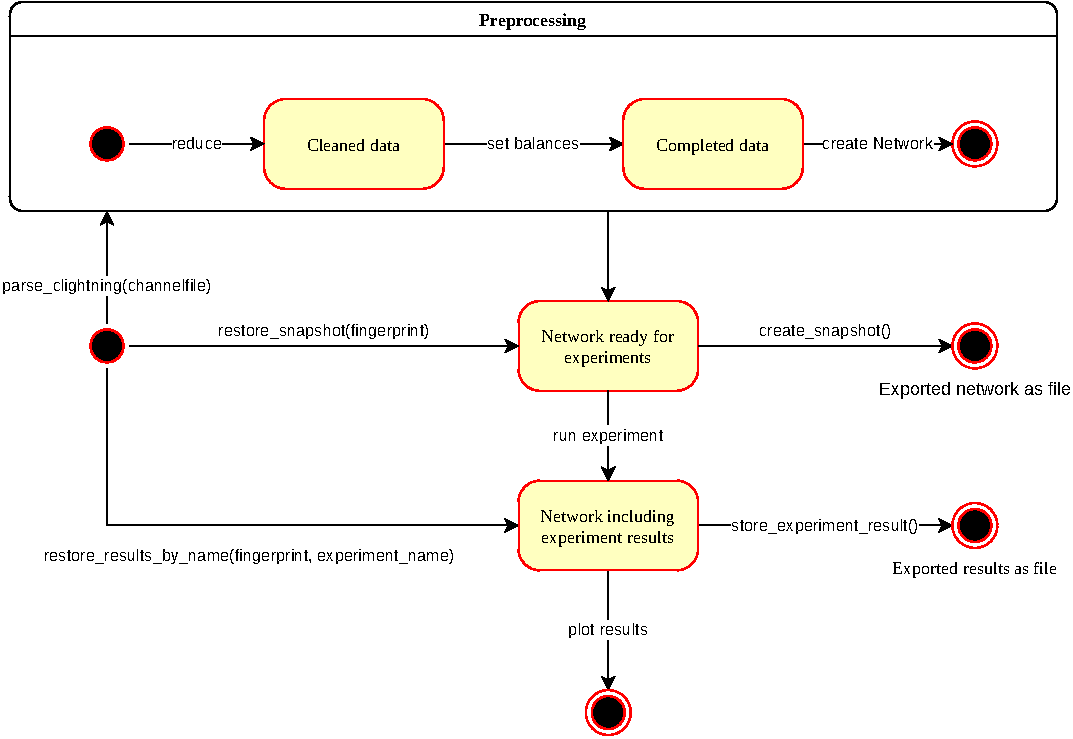
\includegraphics[width=0.9\linewidth]{state_diagram_network.pdf}
\caption{State Diagram of the Network Object}
\label{fig:state_network}
\end{figure}

\subsubsection{Experiment Class}
One experiment is often composed of multiple separate experiments with different parametrisation. The \texttt{Experiment} class is used to interact with those Network objects. This class contains also the definition of an experiment type and takes the parameters as arguments. The different setup methods define the types of experiments available. After the experiment is setup the generic \mintinline{python}{run_experiment()} and \mintinline{python}{plot_experiment()} can be called. Figure~\ref{fig:experiment_class} illustrates the relationship between the classes and shows the public methods of the Experiment class.

\begin{figure}[H]
\centering
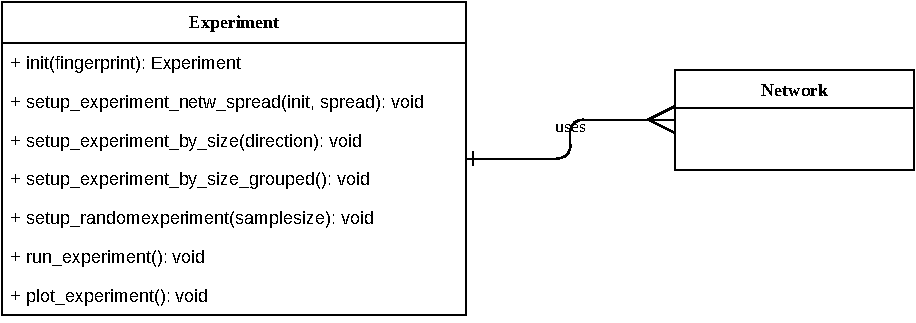
\includegraphics[width=0.7\linewidth]{experiment_network_class.pdf}
\caption{Class Relationship between Experiment and Network}
\label{fig:experiment_class}
\end{figure}

\subsubsection{Command Line Interface}
To simplify the interaction with the simulation software and to facilitate execution of different experimental parameters without the need of changing the source code a simple command-line interface can be used. The file is called \texttt{simulate.py} and uses the package \emph{docopt} to create the interface and the parser. The interface is defined as shown in Listing~\ref{code:cli}. While \texttt{parse} starts the preprocessing from a channel file all other commands execute different types of experiments and take respective parameters. The optional \texttt{---charts} flag skips the experiment and only generates the resulting charts.

\begin{listing}[H]
  \begin{minted}[
  frame=single,
  framesep=3mm,
  linenos=false,
  xleftmargin=21pt,
  tabsize=4,
  breaklines=true,
  breakanywhere=true,
]{bash}
Usage:
  simulate.py parse <filename>
  simulate.py randomexperiment <fingerprint> <samplesize> [--charts]
  simulate.py bysize <fingerprint> [(asc|desc)] [--charts]
  simulate.py groupedsize <fingerprint> [--charts]
  simulate.py spread <fingerprint> <init> <spread> [--charts]
  simulate.py -h | --help
  simulate.py --version

Options:
  -h --help     Show this screen.
  --version     Show version.
  --charts      Skips the experiment and creates only the charts.

\end{minted}
\caption{Description of the command line interface}
\label{code:cli}
\end{listing}

\subsection{Data Collection}\label{subsec:datacol}
Data for the simulation was first collected from a Lightning node. This section describes the data structure obtained and what features were selected as input for the next step, the preprocessing. In this part both terms \emph{key} or \emph{field} are used to refer to the JSON data structure. 

To run a simulation that resembles the real network closely, data from a productive Lightning node are best fitted to construct the model. Lightning is an open network which means it is easy to set up a node and download all the channel information. There are three major implementations of Lightning which technically could deliver the data. The implementation \mbox{C-Lightning} offers a flexible interface to write own plugins which can interact with the node over \gls{rpc}. A Python plugin\footnote{\gitpluginurl} was developed in preparation for the experiments. Employing this plugin all known channels are exported to a JSON file. The code snippet~\ref{code:rawchannel} shows the raw data which is returned by C-Lightning. 

\begin{listing}[H]
\inputminted[
  frame=single,
  framesep=3mm,
  linenos=true,
  xleftmargin=21pt,
  tabsize=4,
  breaklines=true,
  breakanywhere=true,
  highlightlines={4-6,8,14-15},
  highlightcolor=highlightyellow,
]{js}{code/raw.json}
\caption{Raw Channels Extraced from C-Lightning}
\label{code:rawchannel}
\end{listing}

The raw data contains one key named \emph{channels} that represents an array. At the time of data extraction, this array contained 58'934 objects. Nodes can open new channels and close existing ones at any point in time. The state of the network is therefore variable. All experiments conducted in this thesis are based on the local view of my node on July 30, 2020. Each object represents one directed edge. Keys \emph{source} and \emph{destination} refer to the involved node's public key. This public key is used as a pseudonym to preserve the node operator's privacy. Furthermore, private-public key pairs are used to encrypt (see onion Section~\ref{subsec:routing}) and sign messages. Since one entry only represents one directed edge there should be a second entry with the same \texttt{short\_channel\_id} with reversed source-destination nodes to make the bidirectional channel complete. Field \texttt{sathoshis} tells the total channel capacity in the unit sat. The field \texttt{base\_fee\_millisatoshi} is the fixed fee each payment has to pay when routing through the channel. The variable fee to pay for every million satoshis is defined by \texttt{fee\_per\_millionth}. All other fields are not important for the simulation and will be ignored. The plugin extracts the highlighted parts and writes them into a file as shown in Listing~\ref{code:channelbyplugin}. 

Listing~\ref{code:channelbyplugin} shows two entries of the same \texttt{short\_channel\_id} which means they represent the same channel but in opposite directions. Source and destination of both entries confirm this and also the capacity does match. It is also an example of a channel with different fee policies in each direction. For example a payment of $200000$ sat routed from \emph{02ad6f} to \emph{03fab7} would charge no fixed fee but $\frac{200000}{1000000}*1 = 0.2$ sat in variable fee. The same payment routed in the opposite direction would charge the same variable fee but additionally $1000$ msat (equals 1 sat) in fixed fees. So a total of $1,2$ sat. The complete \texttt{channels.json} file can be downloaded from the Github repository. 

\begin{listing}[H]
  \inputminted[
    frame=single,
    framesep=3mm,
    linenos=true,
    xleftmargin=21pt,
    tabsize=4,
    breaklines=true,
    breakanywhere=true
  ]{js}{code/channels.json}
  \caption{Sample Channels File Produced by the Plugin}
  \label{code:channelbyplugin}
\end{listing}
\subsection{Preprocessing}\label{subsec:preproc}
The data obtained in Section~\ref{subsec:datacol} is not yet ready to be used to construct a network. There exist channels in the dataset for which only one of the two edges is known. Furthermore, the information about the distribution of the channel balance is unknown but must be allocated somehow. These two issues are being addressed in the preprocessing which only has to be executed once. The result from the preprocessing is a \mintinline{python}{networkx.DiGraph} which is then passed to the constructor of the Network. It is then accessible through the attribute \mintinline{python}{self.G} of the Network object.

\subsubsection{Remove Incomplete Data}
The data sample presented in Listing~\ref{code:channelbyplugin} shows that each Lightning channel is represented by two entries with opposite source-destination node pairs. In the obtained dataset, not every entry has its matching counterpart. The experiments should only deal with channels that can be used in both direction (normal case), therefore, these data objects are simply deleted from the dataset. This reduced the dataset from a total of 58934 to 46366 (-6172) data objects, representing $\frac{46366}{2}=23183$ channels.  

A \emph{simple directed graph} is used to represent the Lightning network. Multiple edges with the same source and destination node are not permitted. The Lightning protocol does not prevent nodes to open multiple channels with the same partner. Therefore, multiple channels are reduced to one single channel.

\subsubsection{Allocating Local Balances}
The public data only contains information about the total channel capacity, the local distribution between the channel partners is unknown. To run a simulation some distribution must be assumed. As all channels are single funded this means the capacity was all on one side initially. The best guess to distribute channel balances is, therefore, to assume all channels were just opened and therefore only one party hold the full capacity in its balance. However, there is no hint about who opened the channel. This is why the preprocessing allocates 100\% of the capacity to one of the parties \emph{randomly}. To ensure reproducibility of the preprocessing the allocation of the balance should be random but deterministic. Meaning the same channel distributes the capacity to the same node in consecutive runs. Based on the evenness of the result of a \gls{hashfunction} the node holding the balance is selected (see Listing~\ref{code:random_alloc}).

\begin{listing}[H]
  \begin{minted}[
    frame=single,
    framesep=3mm,
    linenos=true,
    xleftmargin=21pt,
    tabsize=4,
    breaklines=true,
    breakanywhere=true,
  ]{python}
# shuffle source<->destination randomly
shuffled = set()
for channel in reduced:
    input = bytearray(channel[0] + channel[1], 'utf-8')
    hash_object = hashlib.sha256(input)
    if hash_object.digest()[0] % 2 == 0:
        shuffled.add(tuple([channel[1], channel[0]]))
    else:
        shuffled.add(channel) 
  \end{minted}
  \caption{Random Allocation of Channel Balance}
  \label{code:random_alloc}
\end{listing}

Depending on the allocation of the balances some nodes are not able to rebalance payments with the rest of the network. To find a network in which each node can reach each other node a NetworkX graph is created with only \emph{one} edge pointing from the node with the balance to the node without balance. From this graph, the \emph{strongly connected component} is selected. This is the directed graph in which a sequence of edges form a path from every vertex to every other vertex \citep{even_network_1975}. The resulting strongly connected component consists of 21147 channels (-2036) and has a diameter of 8.

\subsection{Simulate Rebalancing}\label{subsec:sim_rebal}
Section~\ref{subsec:prop_algo} defined the rebalancing algorithm each node following the protocol change would implement. This section demonstrates how it is implemented in the simulation. Figure~\ref{fig:flow_rebal} serves as a big picture of how such a rebalancing is simulated. The next sections will go into more detail. 

\begin{figure}[H]
\centering
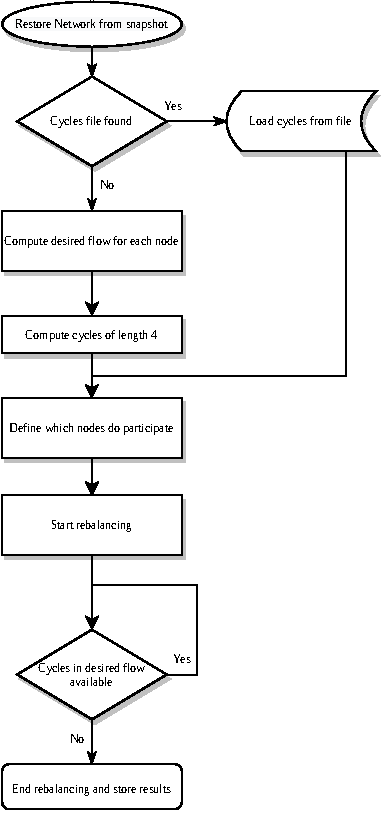
\includegraphics[width=0.7\linewidth]{flow_rebal.pdf}
\caption{Flow Chart of a Rebalancing Experiment}
\label{fig:flow_rebal}
\end{figure}

\subsubsection{Determine the Desired Flow}\label{subsub:flow}
In this step, the amounts all the nodes want to send/receive over any channel is calculated and stored. It is later used to determine possible rebalancing cycles. The method in Listing~\ref{code:comp_flow} covers steps 1 to 4 and part of step 5 described in section ``\nameref{subsec:prop_algo}''.

The method \mintinline{python}{__compute_rebalance_network(self)} creates a new NetworkX graph which is derived from the original network graph (stored in \mintinline{python}{self.G}). Line 4 starts a for-loop which iterates over all edges $(u, v)$ and calculates how much node $u$ would like to send out over this edge. The first step is to calculate the node's \emph{node balance coefficient}. This value is already pre-calculated and can be retrieved from the attributes stored in the NetworkX graph (line 7). Lines 8-10 retrieves the balance and capacity of the edge and calculates the \emph{channel balance coefficient}. The formula from step 5 is used to calculate the amount $a = c(e)\cdot (\zeta_{(u,v)}-\nu_u)$ node $u$ would want to rebalance (line 11). This calculation returns a positive integer which represents the need to send out this amount while a negative integer represents the wish to receive this amount. 

Since a payment channel is always represented by two edges two nodes have some different need to rebalance it. As the protocol foresees only rebalance transactions from which both benefit, an agreement must be found. In case both nodes would want to rebalance into different directions (both want to send or receive at the same time) the channel is completely removed from the flow graph. As in the replicated network, all channel balance lies on one end of the channel this will not be the case. However, most likely one of the nodes wants to send more than the counterparty wants to receive (or the other way around). This case is handled in lines 12-19. The lower of the two values is taken and stored into the flow graph with respect to the sign.

The result of this procedure is a property \mintinline{python}{self.flow} which contains a network graph that has two opposite directed edges for each channel that wants to be rebalanced by both parties. The amount stored in the attribute \texttt{liquidity} is the lower value on which the channel partners could agree on. The value is the same for edges of a channel, but positive on the edge that wants to send and negative on the one that wants to receive. This flow graph will be used later to compute possible rebalancing paths. 

\begin{listing}[H]
  \begin{minted}[
    frame=single,
    framesep=3mm,
    linenos=true,
    xleftmargin=21pt,
    tabsize=4,
    breaklines=true,
    breakanywhere=true,
  ]{python}
 def __compute_rebalance_network(self):
        self.flow = nx.DiGraph()
        delete_edges = []
        for u, v in self.G.edges():
            if u in self.__excluded or v in self.__excluded:
                continue
            nbc = self.G.nodes[u]['nbc']
            balance = self.G[u][v]['balance']
            capacity = self.G[u][v]['capacity']
            cbc = balance / capacity
            amt = int(capacity * (cbc - nbc))
            if (v, u) in self.flow.edges():
                amt_cp = self.flow[v][u]['liquidity']
                if np.sign(amt) == np.sign(amt_cp):
                    ...
                common = min(abs(amt), abs(amt_cp))
                amt_cp = common * np.sign(amt_cp)
                amt = common * np.sign(amt)
                self.flow[v][u]['liquidity'] = amt_cp
            self.flow.add_edge(u, v, liquidity=amt)
  \end{minted}
  \caption{Method to Calculate Each Nodes Willingness to Rebalance}
  \label{code:comp_flow}
\end{listing}

\subsubsection{Compute Rebalancing Cycle}
Step 5 of the rebalancing algorithm tells a node $u$ to construct circular payments using a path $p = [v,x_1,\dots,x_n,u]$ for which $\zeta_{(u,v)}>\nu_u$ and $\zeta_{(x_n,u)}<\nu_u$. Such a rebalancing transaction helps a node to adjust both channel balance coefficients towards the node balance coefficient. In the real network nodes would individually calculate those paths based on the \emph{rebalancing hints} they receive from their local neighbourhood. The simulation already has this holistic view since the desired flow was already calculated in Section~\ref{subsub:flow}. 

The previously calculated flow network indicates the direction in which nodes want to rebalance. We can now simply extract all cycles of length 4 or 3 from that graph as shown in the method \mintinline{python}{compute_circles()} in Listing~\ref{code:comp_circles}. 

Line 4-6 create an extract of the flow network with only positive edges. The negative edges are just the counterparts of the same size in the opposite direction and can be deleted. Lines 7-9 then iterate over each edge $e = (u, v)$ and use the built-in function \mintinline{python}{networkx.all_simple_paths()} to find all paths from $v$ to $u$. The \emph{cutoff parameter} 3 specifies the maximum length of paths returned. To build cycles of length 4 the cutoff is specified as 3 as the edge $e = (u, v)$ is later added to make it a full circle. Since node $u$ is always the last node in the found path it does not have to be stored at this stage. All found cycles are then randomly ordered in a deterministic manner and stored to a file. 

During the future rebalancing process, those set of circular paths will not change as channels will never become less balanced. This means the liquidity in the flow network only decreases and edges might disappear completely, but new edges cannot appear. This fact is very helpful since the heavy computation of the paths needs to be done only once. If during the restore procedure an existing file of exported paths is found, this will be automatically imported.

\begin{listing}[H]
  \begin{minted}[
    frame=single,
    framesep=3mm,
    linenos=true,
    xleftmargin=21pt,
    tabsize=4,
    breaklines=true,
    breakanywhere=true,
  ]{python}
    def compute_circles(self, force=False):
        ...
        cycles4 = []
        pos_edges = [e for e in self.flow.edges(data=True) if e[2]['liquidity'] > 0]
        pos_flow = nx.DiGraph()
        pos_flow.add_edges_from(pos_edges)
        for i, (u, v) in enumerate(pos_flow.edges):
            paths = [p for p in nx.all_simple_paths(pos_flow, v, u, 3)]
            [cycles4.append(p) for p in paths if len(p) <= 4]
        ...
        self.__cycles4 = cycles4
        random.seed(10)
        self.__cycles4.sort()
        random.shuffle(self.__cycles4)
        self.__store_cycles()
  \end{minted}
  \caption{Extracts Cycles of Length 4 (or less) from the Flow Graph}
  \label{code:comp_circles}
\end{listing}

\subsubsection{Node Selection}
The main question that should be answered by the experiments is how the proposed rebalancing algorithm behaves if only a part of the entire network participates. For each level of participation, an individual experiment is conducted and the nodes that should be excluded have to be defined. The selection strategies are explained in Section~\ref{subsec:selstrat}.

The selection strategy is implemented in the \texttt{Experiment} class and then calls the \mintinline[breaklines, breakafter=(]{python}{exclude(excl_list)} method of the Network object. The passed parameter is a list of nodes which will not participate in the rebalancing. Those nodes are stored in a local variable for later lookups. Furthermore, all the cycles which are precalculated need to be adapted. Listing~\ref{code:reduc_cyc} combines a list comprehension combined with a boolean set comparison. A set is a data structure in which each element can only be contained once. They allow for fast membership operations. Each path in \mintinline{python}{self.__cycles4} is converted to a set and then intersected with another set \mintinline{python}{self.__excluded}. If at least one of the nodes in the path is also excluded, the result is a non-empty set. Only paths with no excluded nodes in it should be kept which is checked with the boolean comparison \mintinline{python}{if not}.  

\begin{listing}[H]
  \begin{minted}[
    frame=single,
    framesep=3mm,
    linenos=true,
    xleftmargin=21pt,
    tabsize=4,
    breaklines=true,
    breakanywhere=true,
  ]{python}
def exclude(self, excl_list):
        ...
        self.__excluded = set(excl_list)
        cycles4 = [c for c in self.__cycles4 if not (set(c) & self.__excluded)]
        self.__cycles4 = cycles4
        ...
  \end{minted}
  \caption{Reduction of the Available Rebalancing Cycles}
  \label{code:reduc_cyc}
\end{listing}


\subsubsection{Execute Rebalancing}
Once the excluded nodes are defined and the rebalancing paths are adjusted the actual rebalancing experiment can be started. To be able to track the results throughout the experiment intermediate results are also calculated and stored. 

The \mintinline{python}{rebalance()} method start this process that runs until either no more payments can be done or the upper threshold (default: $100000$) is reached. This process iterates over all available rebalance cycles and simulates payments with the maximum possible size all nodes can agree to rebalance. This amount is found by taking the lowest \texttt{liquidity} attribute of the edges in the flow network. If this amount is at least one sat, the rebalancing operation is executed. 

\begin{listing}[H]
  \begin{minted}[
    frame=single,
    framesep=3mm,
    linenos=true,
    xleftmargin=21pt,
    tabsize=4,
    breaklines=true,
    breakanywhere=true,
  ]{python}
def __update_channel(self, tx, rev=False):
        amount = tx[0] if not rev else tx[0] * -1
        circle = tx[1]
        for i in range(len(circle) - 1):
            src = circle[i]
            dest = circle[i + 1]
            self.G[src][dest]['balance'] -= amount
            self.G[dest][src]['balance'] += amount
            self.flow[src][dest]['liquidity'] -= amount
            self.flow[dest][src]['liquidity'] += amount
        [self.__update_node_gini(n) for n in circle[:-1]]
  \end{minted}
  \caption{Record Each Rebalancing Payment}
  \label{code:record}
\end{listing}

Listing~\ref{code:record} shows how a rebalancing transaction is reflected in the two networks \mintinline{python}{self.G} (state of the Lightning Network) and \mintinline{python}{self.flow} (desire to rebalance). The input parameter \mintinline{python}{tx} is a tuple containing the amount and the circle. Line 4 iterates through each hop and determines the source and destination node of that hop. Since payment through a channel redistributes the local balances, both edges representing one channel have to be updated. Line 7 \& 8 increase and decrease the balances by the payment amount. Similarly, the desire to rebalance represented in the flow network must be adjusted. Each payment changes the balance-distribution of the involved nodes. In order to determine the new balance measure, the \gls{gini} coefficient, the \mintinline{python}{self.__update_node_gini(n)} is called for each node that was involved in the payment (line 11).

To later analyse how the network's ability to route payments improve while the network becomes more balanced, different performance measures (defined in Section~\ref{sub:perfm}) are calculated. As they take a while to calculate this is not done after every payment but only when the \gls{gini} coefficient improves by $0.01$.

\subsubsection{Store and Plot Results}
After all rebalancing operations are performed the results should be stored to later allow to generate different data visualisations. Multiple files will be generated containing all the necessary data. The plots of the results often combine multiple networks with different participation, hence, can not be executed by the Network class. The selection of the desired data series and the creation of plots is handled by the \texttt{Experiment} class.

\section{Results}\label{sec:result}
The results of all the previously presented experiments are presented in this section. The main focus is put on the performance measures defined in Section~\ref{sub:perfm}. The main tool for analysing and interpreting the results are charts which visualise the measures with different levels of node participation.

\subsection{Random Participation}
Before analysing the performance measures the change of the balance score (\gls{gini}) during the process of rebalancing will be observed. Figure~\ref{fig:gini_rebal_rand} compares the \gls{gini} score with the number of rebalancing operations executed. It becomes evident that smaller participation of nodes leads to a decreased amount of rebalancing operations. This is because rebalancing only occurs between nodes which participate in the new protocol. If only one node within a cycle is not participating the whole cycle is ignored. The decreasing slope of the \gls{gini}, and therefore rate of increase in the balance of the network, is similar among the different participation levels. Thus, follows that the fewer rebalancing possibilities are responsible for the smaller balance improvement. 

\begin{figure}[H]
\centering
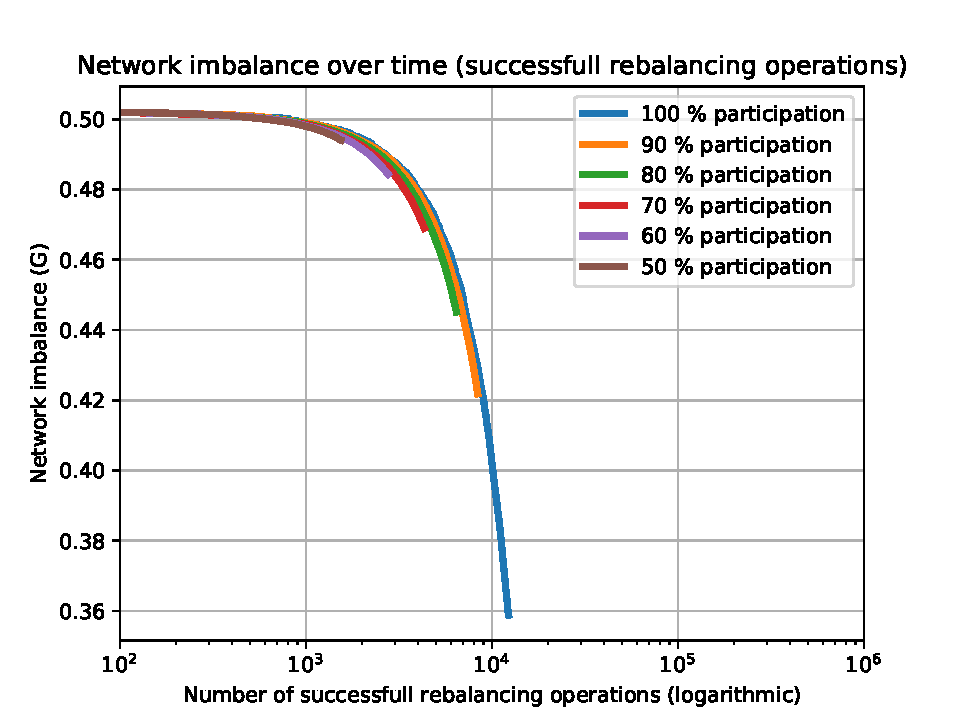
\includegraphics[width=0.7\linewidth]{results/3a65a961_gini_vs_rebalops_random.pdf}
\caption{Compare Development of \gls{gini} Score During Rebalancing}
\label{fig:gini_rebal_rand}
\end{figure}

Since fewer rebalancing opportunities results in a smaller \gls{gini} score, the best \gls{gini} score a network can achieve is lower the fewer nodes participate. Figure~\ref{fig:gini_part_rand} shows this relation. The yellow area around the mean \gls{gini} score visualises the standard deviation of the 10 experiments conducted with different random node selections. There must be no standard deviation at 100\% since the node selection is always the same. Furthermore, the deviation is very small in the low bands of participation which signals a low \gls{gini} score no matter what nodes are selected. 

Note the second Y-axis which shows the relative capacity that participates at different node participation levels. This indicates how much of the channel capacity was available for rebalancing. As more nodes will contribute more capacity, node participation and capacity participation must be monotonically increasing. But the rate at which it increases reveals some insight about the effect of the different node selection methods. 

\begin{figure}[H]
\centering
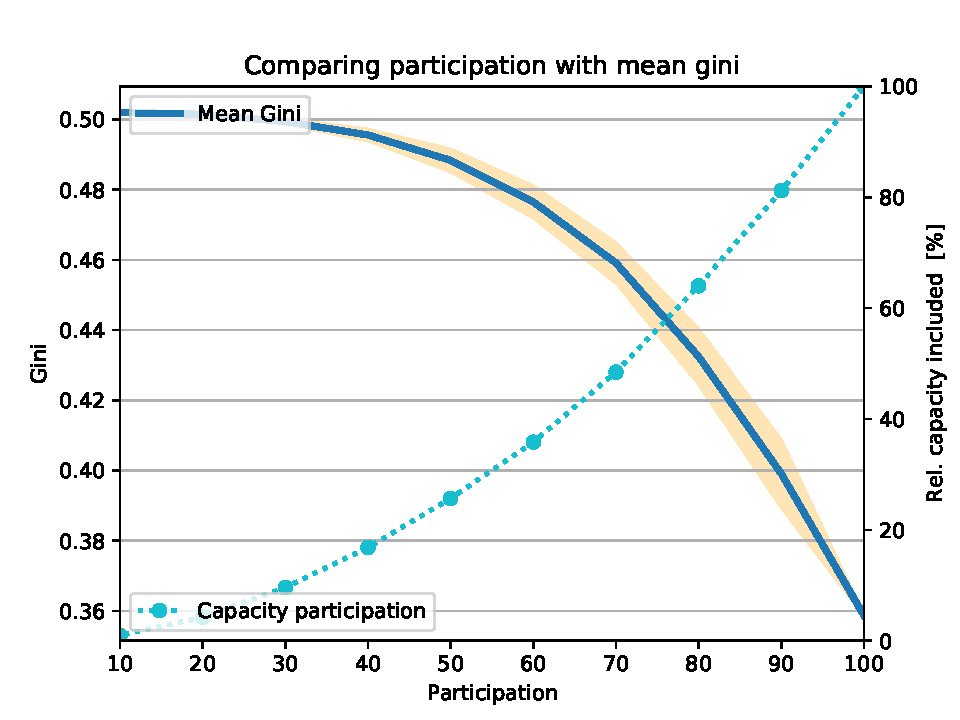
\includegraphics[width=0.7\linewidth]{results/3a65a961_gini_vs_participation_random.pdf}
\caption{Compare Final \gls{gini} Score with Participation Level}
\label{fig:gini_part_rand}
\end{figure}

The two charts in Figure~\ref{fig:pay_size_random} show the first performance measure \gls{mps} at different \gls{gini} levels and also for the different levels of participation. Since the variable is not evenly distributed, a median value will usually generate certain spikes. Both charts visualise that an improvement of the measure is only noticeable with a participation of 80\% or higher. 
\begin{figure}[htp]
\centering
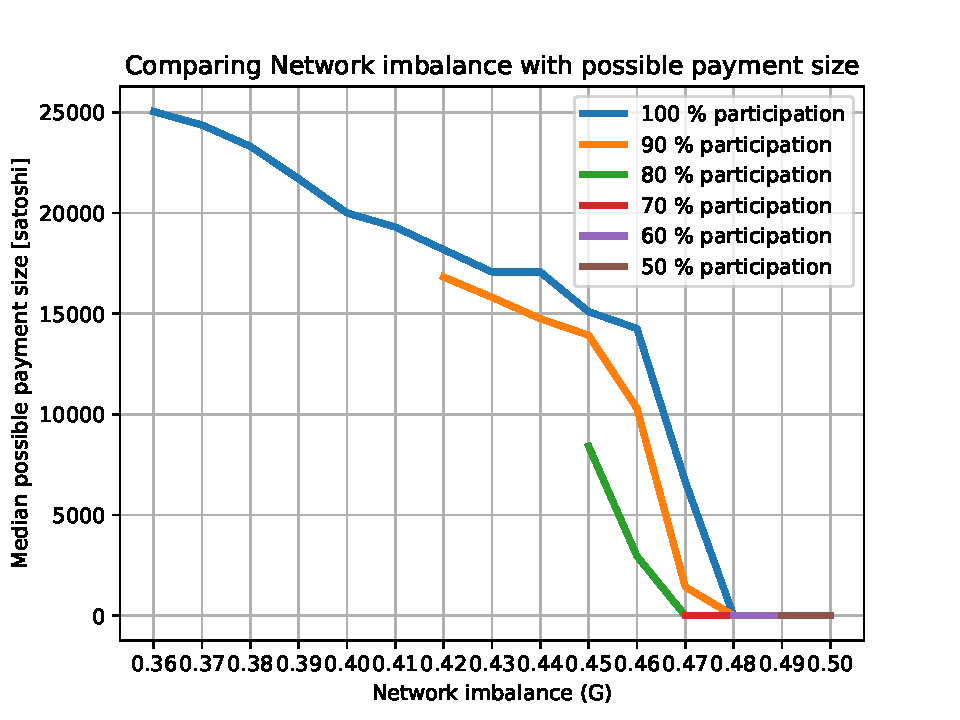
\includegraphics[width=.5\textwidth]{results/3a65a961_median_payment_size_random.pdf}\hfill
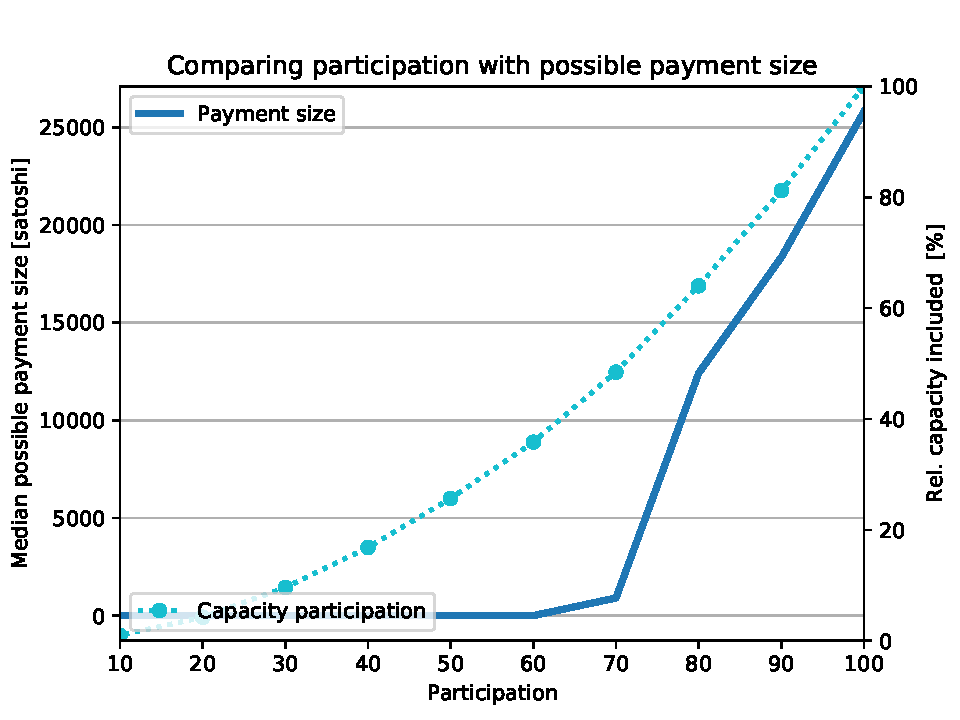
\includegraphics[width=.5\textwidth]{results/3a65a961_median_paymnet_size_vs_participation_random.pdf}
\caption{\gls{mps} in Random Node Selection}
\label{fig:pay_size_random}
\end{figure}

A similar picture can be drawn from the \gls{sr} measure. Since this is the ratio of all node pairs able to rout at least 1 sat there are no spikes. The improving effects are more distributed among the different levels of participation. The imbalanced network already has a \gls{sr} of 20\% which can be improved further up to 80\% (under total participation).

It can be seen that at a given \gls{gini} score, the performance measure is lower for lower participation levels. This reveals the limitation of the \gls{gini} score as a \gls{proxy} for the network's balance.

\begin{figure}[htp]
\centering
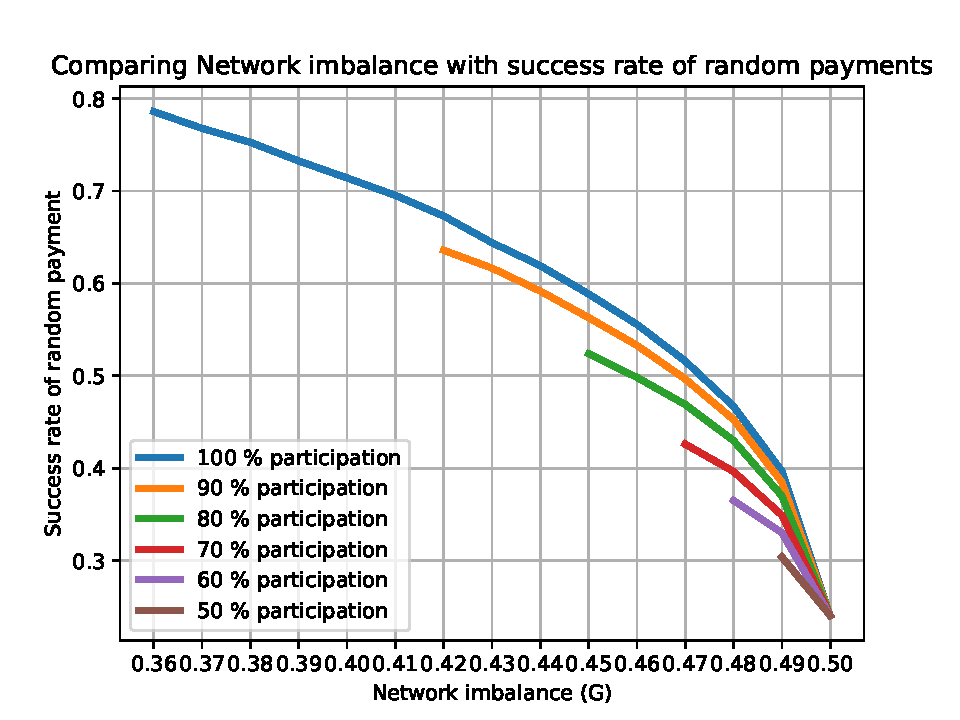
\includegraphics[width=.5\textwidth]{results/3a65a961_successrate_vs_imbalance_random.pdf}\hfill
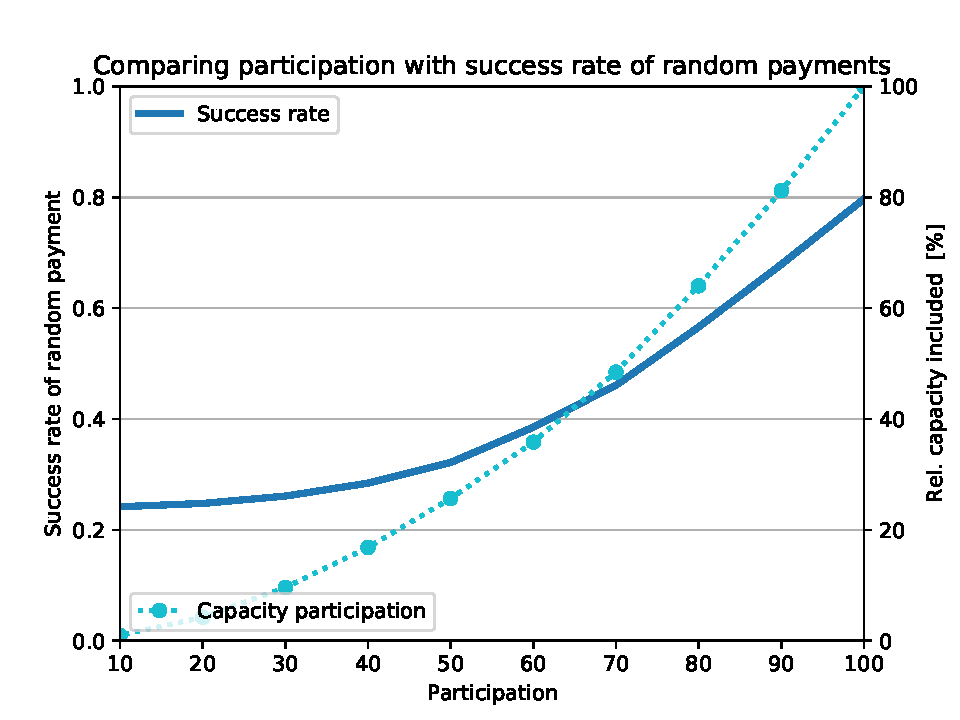
\includegraphics[width=.5\textwidth]{results/3a65a961_successrate_vs_participation_random.pdf}
\caption{\gls{sr} in Random Node Selection}
\label{fig:success_random}
\end{figure}

Figure~\ref{fig:sizes_random} compares the third performance measure, \gls{mpr}, that evaluates how many paths out of 10 between each node pair can accommodate a payment of a certain size. The ability to send a micropayment of the size 10'000 sat increases roughly the same as the ability to send 1 sat. Hence, can be concluded that the ability to send 1 sat leads to the ability to also send 10'000 sat respectively. 

\begin{figure}[htp]
\centering
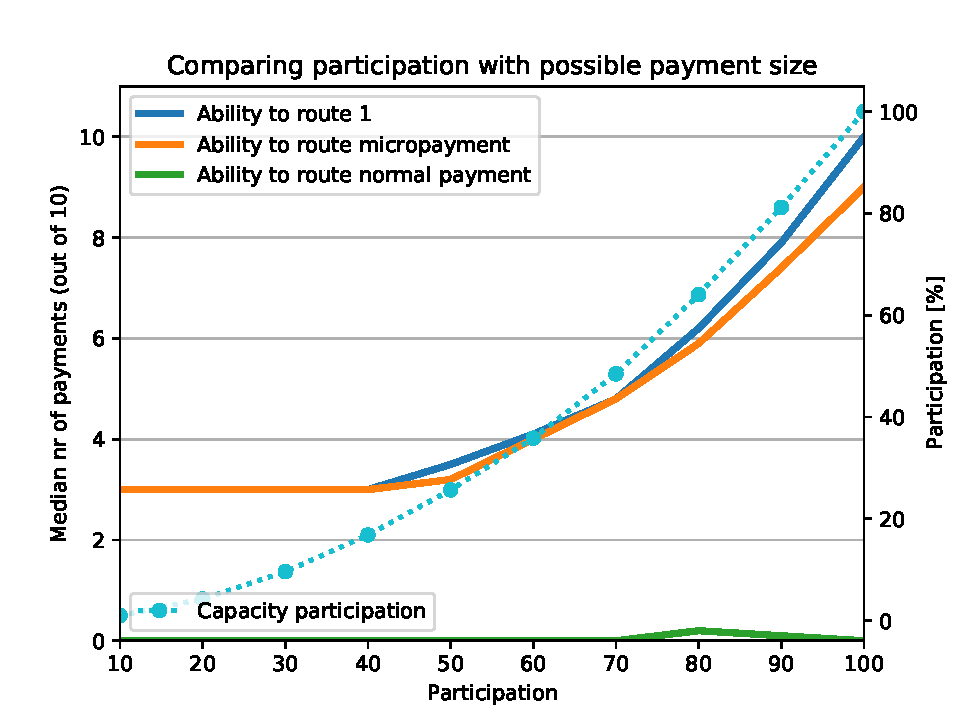
\includegraphics[width=.7\textwidth]{results/3a65a961_median_paymnets_vs_participation_random.pdf}
\caption{\gls{mpr} in Random Node Selection}
\label{fig:sizes_random}
\end{figure}

\subsection{Node Importance}
\subsubsection{Adoption by Important Nodes First}\label{subsub:desc}
This section shows the results for the experiments for which the participating nodes were chosen based on their importance ranking. The fraction of participating nodes were chosen from the highest-ranked nodes. 

The fact persists that lower participation results in lower performance measures as can be seen in Figures~\ref{fig:pay_size_size_linear_desc} and \ref{fig:success_size_linear_desc}. From the dotted line representing the fraction of the total capacity that participates, it is also visible that those important nodes contribute overproportionately to the available capacity. 30\% of nodes include 80\% of the capacity and 50\% include 90\%. This explains why the \gls{gini} score falls much faster with increasing participation than it was the case with random selection.

\begin{figure}[H]
\centering
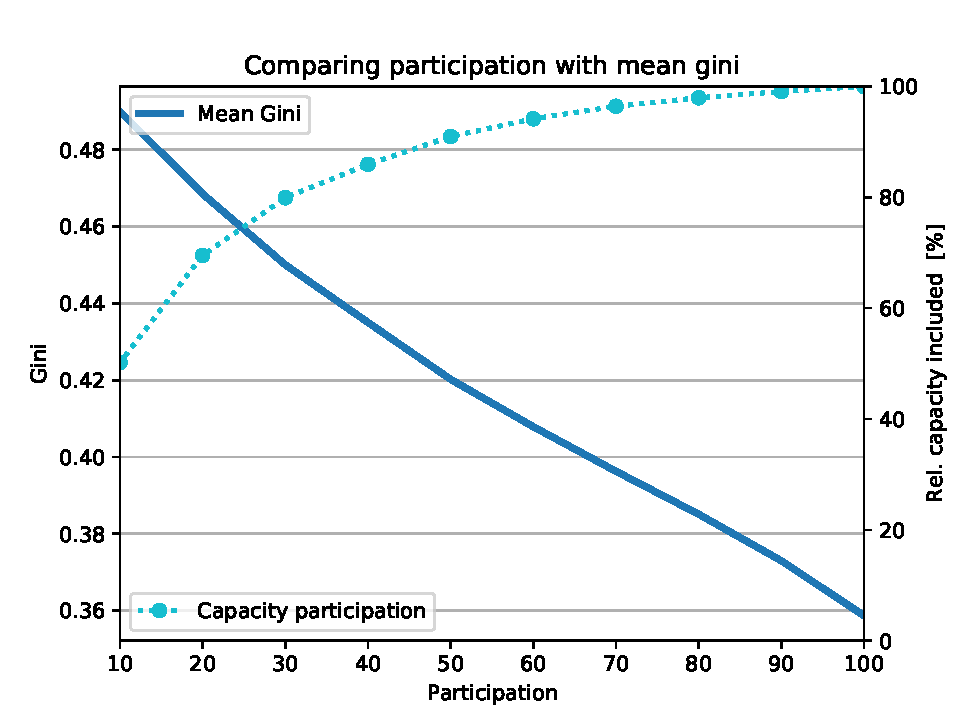
\includegraphics[width=0.7\linewidth]{results/3a65a961_gini_vs_participation_size_linear_desc.pdf}
\caption{\gls{gini} Score with Node Selection: Important Nodes First}
\label{fig:gini_part_size_linear_desc}
\end{figure}

This lower \gls{gini} score has its effect on the performance measures which are consistently higher in all levels of participation. The \gls{mps} measure seen in Figure~\ref{fig:pay_size_size_linear_desc} already increases steeply with 40\% compared to 80\% with random selection.

\begin{figure}[htp]
\centering
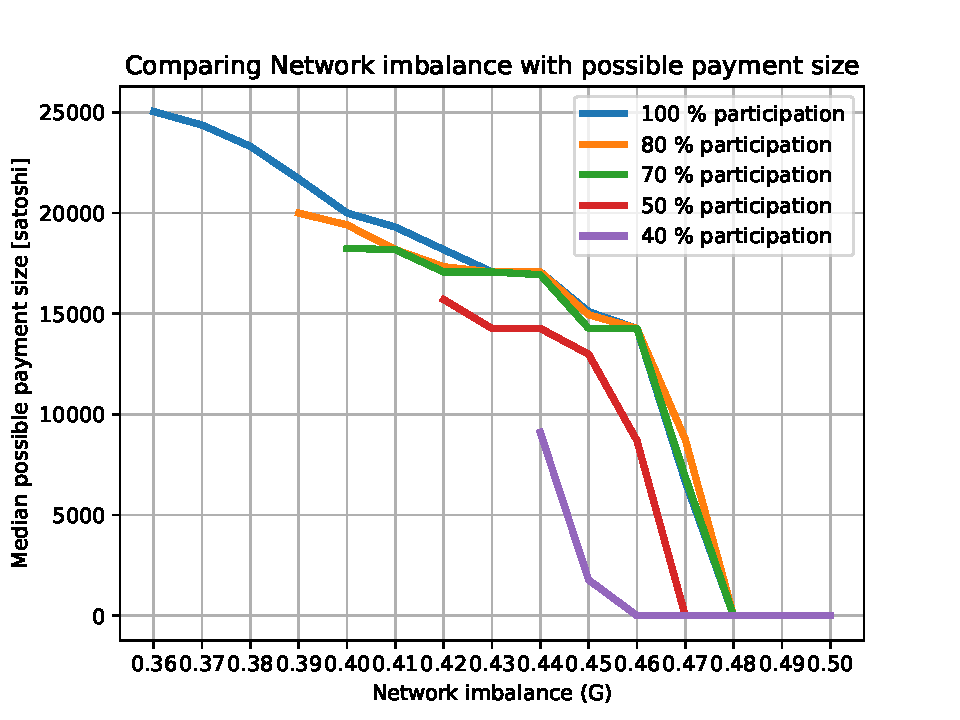
\includegraphics[width=.5\textwidth]{results/3a65a961_median_payment_size_size_linear_desc.pdf}\hfill
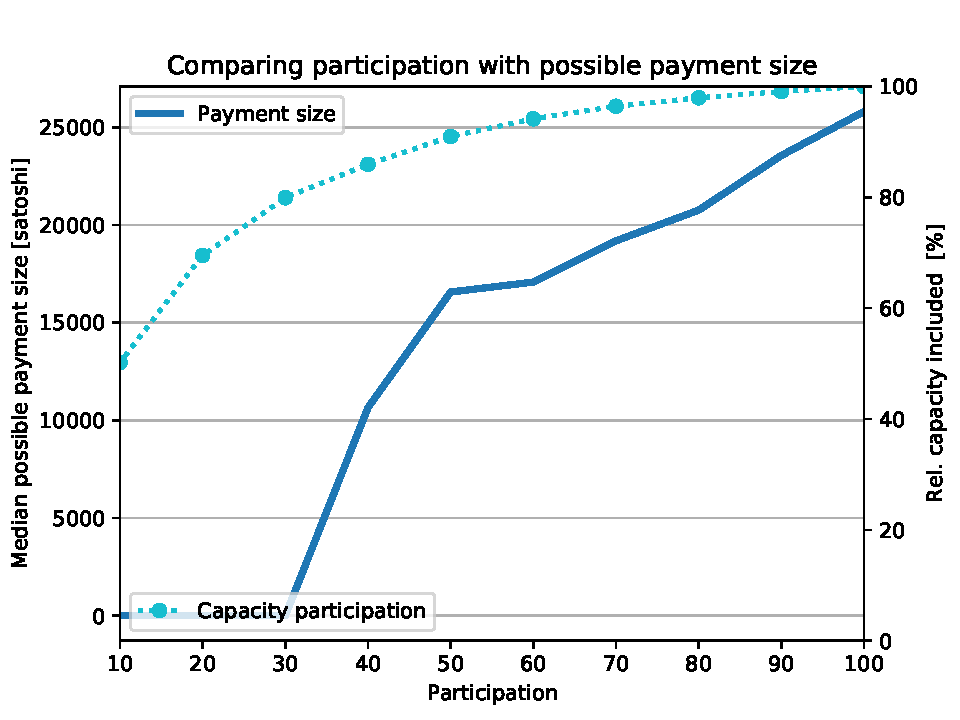
\includegraphics[width=.5\textwidth]{results/3a65a961_median_paymnet_size_vs_participation_size_linear_desc.pdf}
\caption{\gls{mps} with Node Selection: Important Nodes First}
\label{fig:pay_size_size_linear_desc}
\end{figure}


The \gls{sr} in Figure~\ref{fig:success_size_linear_desc} is already with 10\% participation almost two times higher than with random selection. It then grows linearly to the same levels of 80\%.

\begin{figure}[htp]
\centering
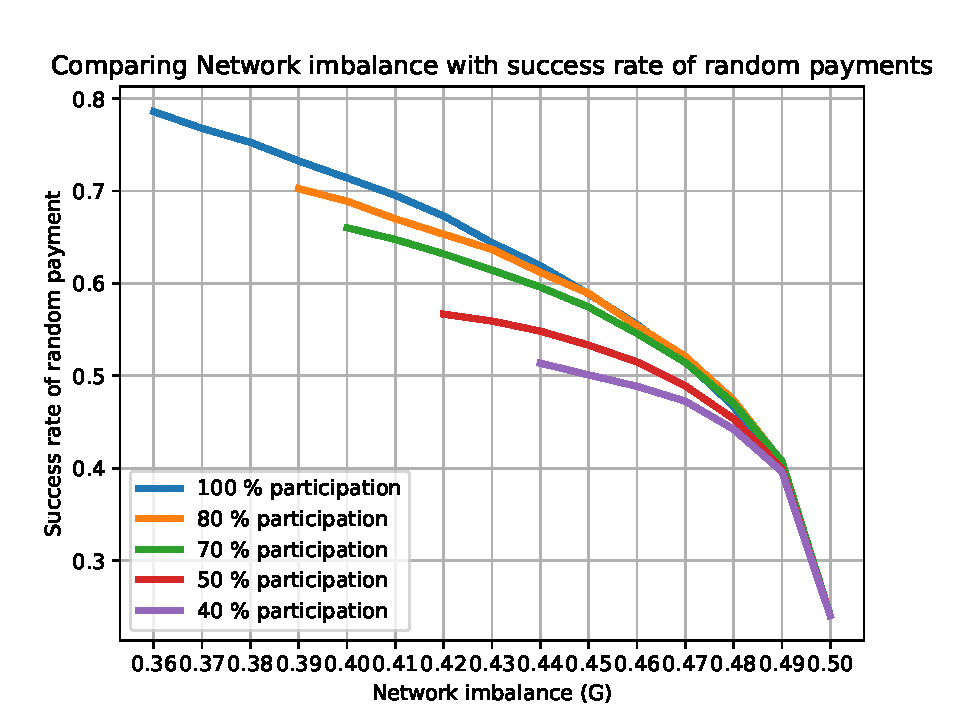
\includegraphics[width=.5\textwidth]{results/3a65a961_successrate_vs_imbalance_size_linear_desc.pdf}\hfill
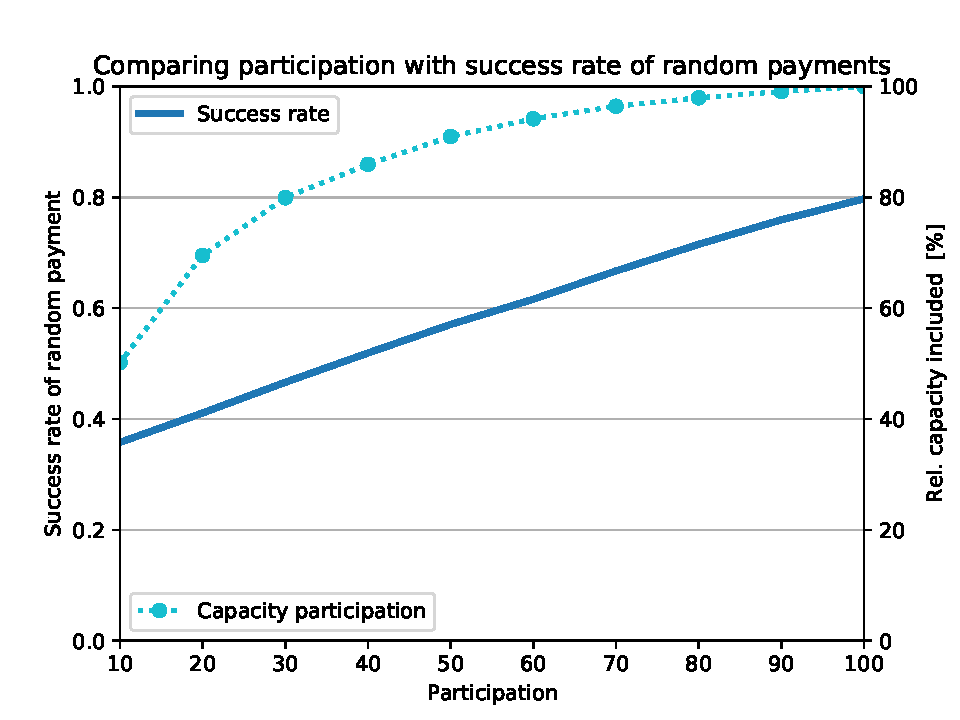
\includegraphics[width=.5\textwidth]{results/3a65a961_successrate_vs_participation_size_linear_desc.pdf}
\caption{\gls{sr} with Node Selection: Important Nodes First}
\label{fig:success_size_linear_desc}
\end{figure}

Also, the ability to route certain payments is much better with lower participation. A 50\% participation already allows 8 out of 10 payments up to 10'000 sat to succeed. The random selection needed 90\% participation to reach a similar result. A payment of the size 100'000 sat never got routed. Therefore, no conclusion can be drawn from the data.

\begin{figure}[htp]
\centering
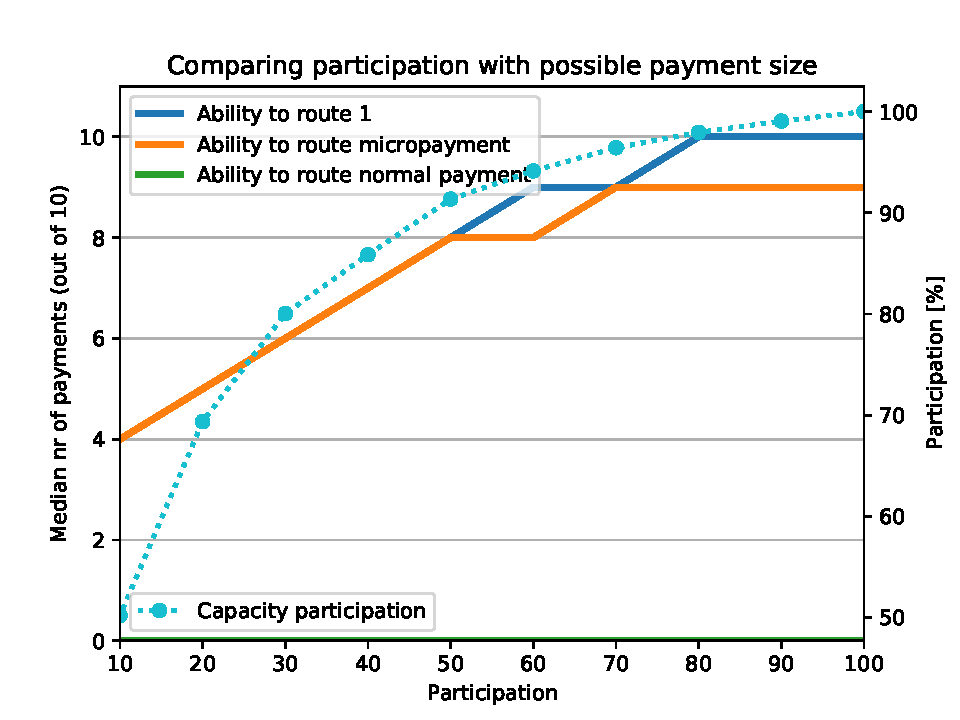
\includegraphics[width=.7\textwidth]{results/3a65a961_median_paymnets_vs_participation_size_linear_desc.pdf}
\caption{\gls{mpr} with Node Selection: Important Nodes First}
\label{fig:sizes_size_linear_desc}
\end{figure}


\subsubsection{Adoption by Unimportant Nodes First}\label{subsub:asc}
Instead of the top-ranked nodes, this part covers the selection from the lowest-ranked nodes. The result shows that all participation levels of less than 100\% did not improve the network's balance at all. This is why an additional experiment was conducted with 95\% participation. But even then, no improvement in the \gls{gini} score could be recorded, as shown in Figure~\ref{fig:gini_part_size_linear_asc}.

\begin{figure}[htp]
\centering
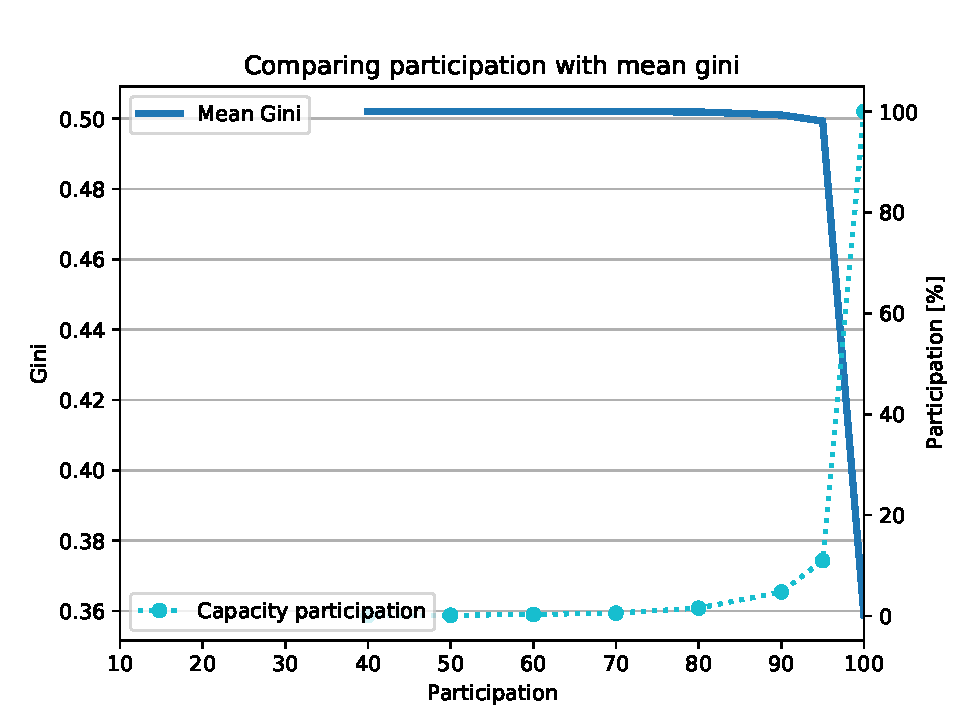
\includegraphics[width=.7\textwidth]{results/3a65a961_gini_vs_participation_size_linear_asc.pdf}
\caption{\gls{gini} Score with Node Selection: Unmportant Nodes First}
\label{fig:gini_part_size_linear_asc}
\end{figure}

One reason for this could be the ratio of channel capacity that was available for the rebalancing. As displayed in Figure~\ref{fig:gini_part_size_linear_asc}, capacity only slowly starts rising at levels of 90\%. Even 95\% of all nodes only contribute 11\% of capacity. 

Another conclusion would be that most of the unimportant nodes are not well connected with each other but mainly with central nodes. This would lead them to be disconnected as soon as the most central nodes are no longer available. This, in turn, eliminates most of the rebalancing cycles and avoids any improvement. To make clearer statements about the situation, a more detailed analysis of the network topology is needed.

\subsubsection{Participation Within a Group}
When the experiment was conducted with equal frequency binning with regards to nodes the three groups each contained 713 nodes. As the previous results from Section~\ref{subsub:asc} have shown, even the 95\% lowest-ranked nodes are not able to rebalance a significant amount and therefore did not improve the performance measures. Concluding, both the low and the intermediate group also are not able to improve the network's balance at all even when the entire group participates. Successive experiments with lower participation in those groups were meaningless. The group containing the 713 most important nodes does, of course, result in some rebalancing, however, this leads to the same result as in Section~\ref{subsub:desc} just with an increased granularity (of factor three).

\subsection{Network Spread}
The results from the experiments stemming from the selection via network spread do not vary significantly from the randomly selected ones. This can be explained that both, the initial set of starting nodes as well as the ones added during each iteration are chosen randomly as well. So, the results regarding the performance measures of the network are similar to those. What can be learned, however, is the influence of the two experimental parameters on the participation levels of nodes and capacities.

When an experiment with low \emph{initial value} is compared to one with high \emph{initial value} surely results in the first iterations are better. The higher participation, in the beginning, acts as a head-start. However, they do not diverge much in the number of iterations it takes to achieve high network saturation. The head-start starts to diminish throughout further iterations as can be observed in Figure~\ref{fig:fix_spread}.

\begin{figure}[htp]
\centering
  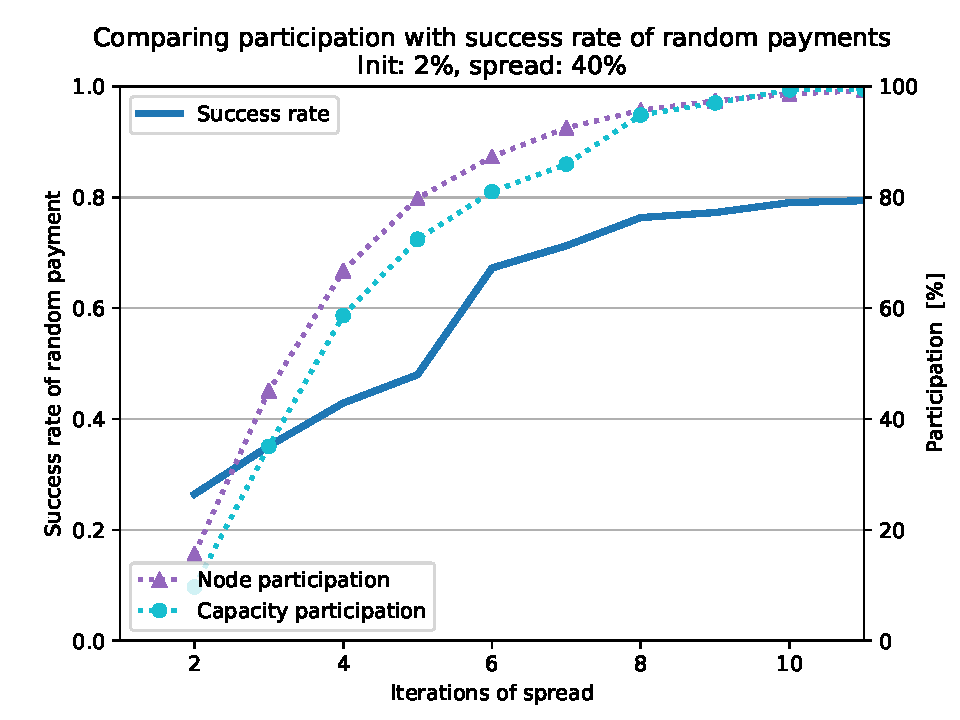
\includegraphics[width=60mm]{results/3a65a961_successrate_vs_participation_netw_spread_02_40.pdf} 
  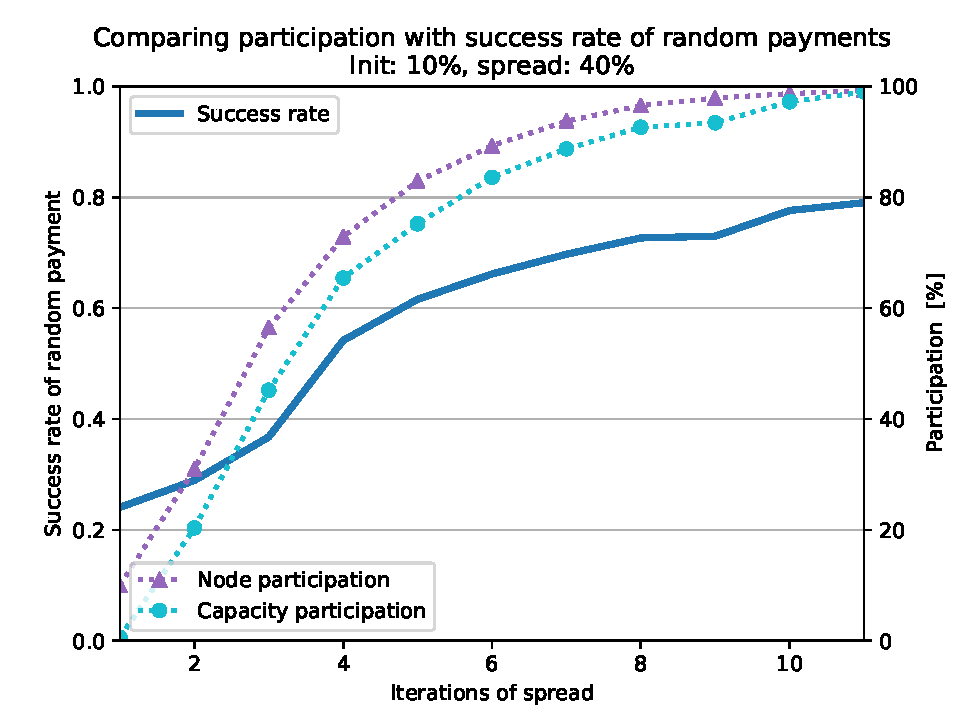
\includegraphics[width=60mm]{results/3a65a961_successrate_vs_participation_netw_spread_10_40.pdf} 
  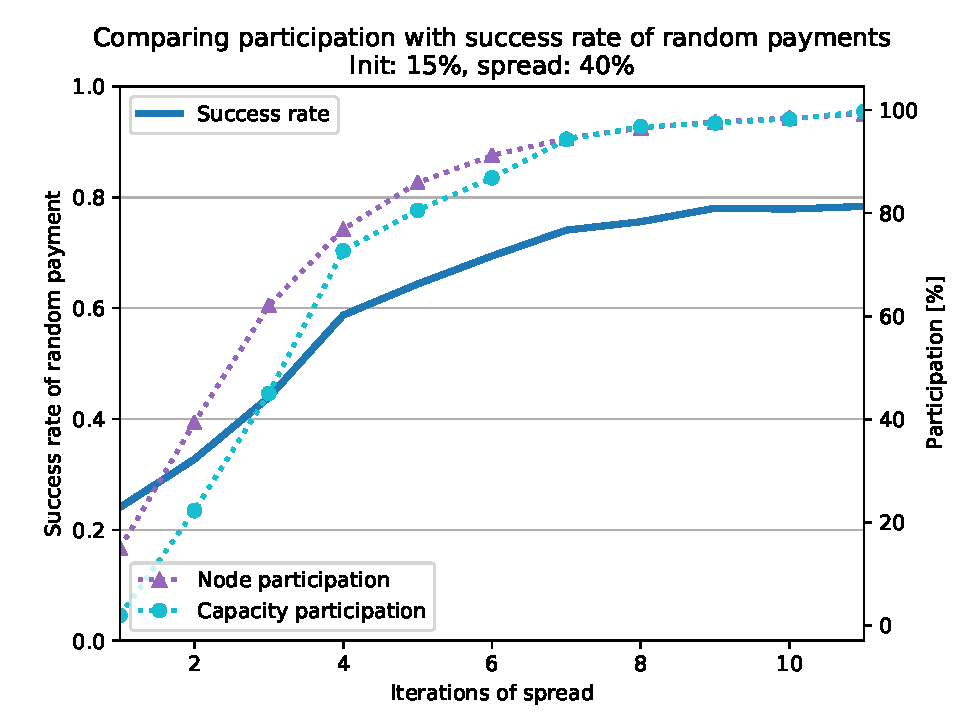
\includegraphics[width=60mm]{results/3a65a961_successrate_vs_participation_netw_spread_15_40.pdf}
\caption{\gls{sr} With Different Init Parameters and a Fixed Spread of 40\%}
\label{fig:fix_spread}
\end{figure}

However, when low and high \emph{spread} is compared, the number of iterations to reach a 99\% coverage is reduced by four. The development of the different measures does not vary much, simply the rate at which they progress. Figure~\ref{fig:fix_init} shows how the speed of spread is increased. The visualisation of the results with all parametrisations can be found in Figures \ref{fig:sr_all_spread}, \ref{fig:mps_all_spread}, \ref{fig:mpr_all_spread} and \ref{fig:gini_all_spread} which are part of the appendix.


\newpage
\begin{figure}[htp]
\centering
  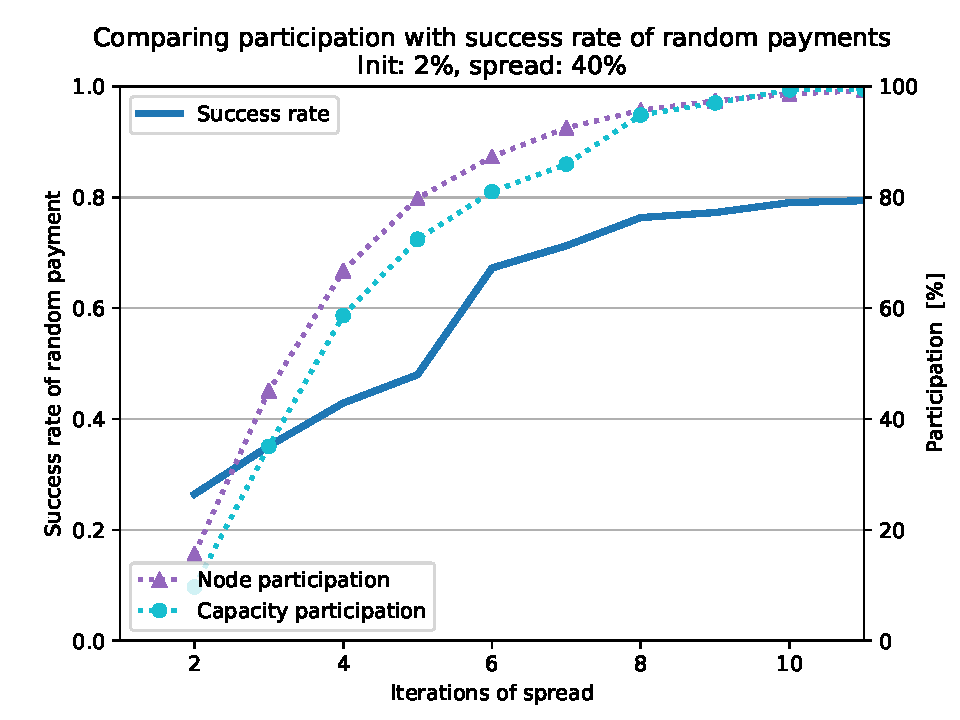
\includegraphics[width=60mm]{results/3a65a961_successrate_vs_participation_netw_spread_02_40.pdf} 
  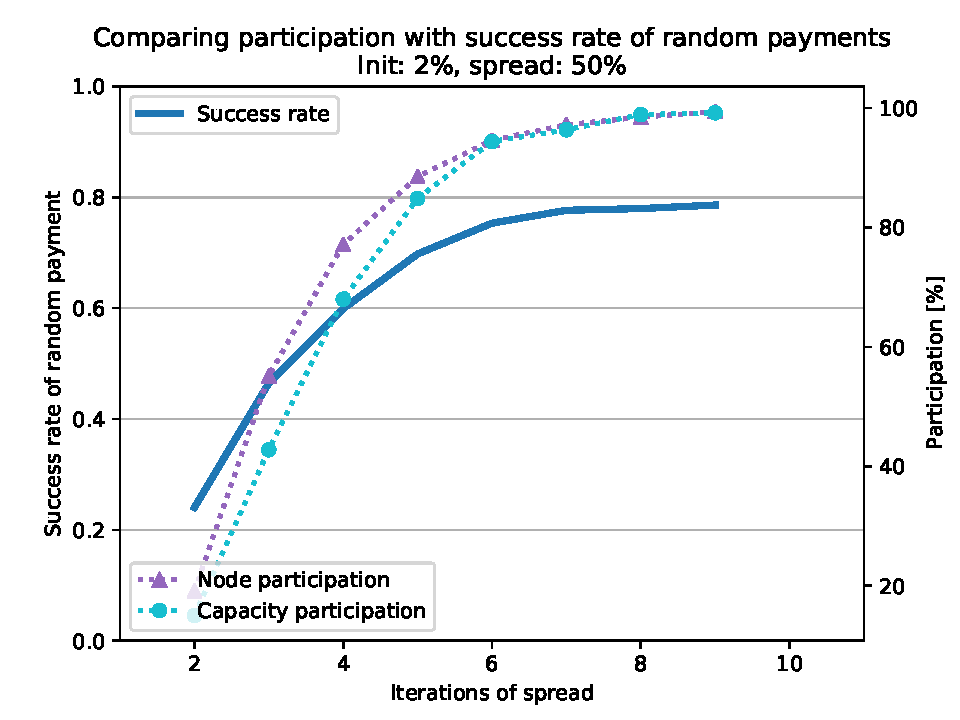
\includegraphics[width=60mm]{results/3a65a961_successrate_vs_participation_netw_spread_02_50.pdf} 
  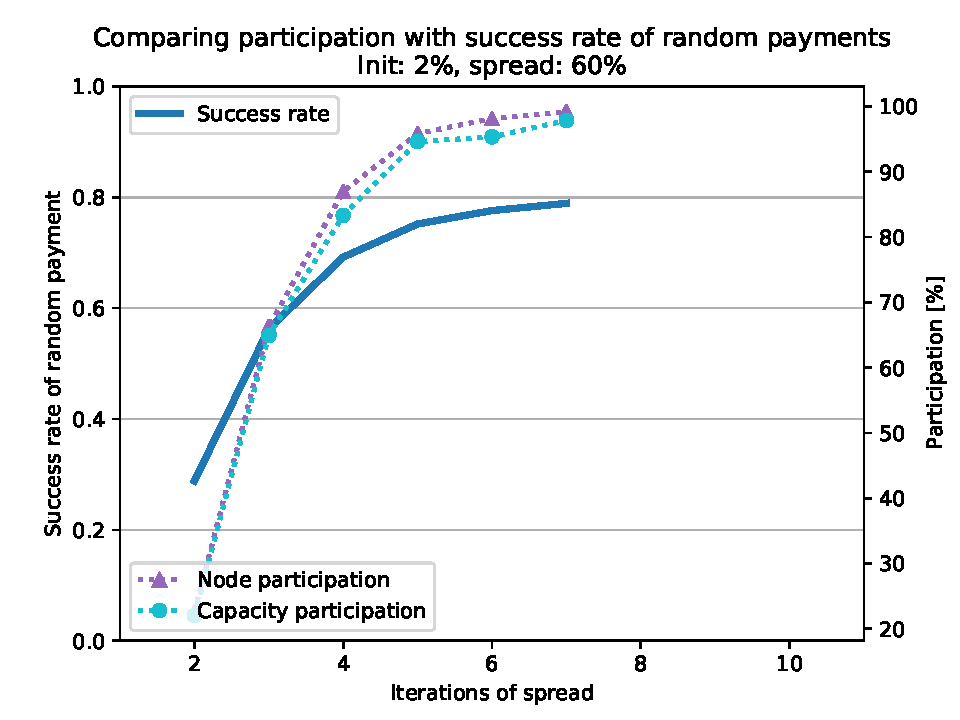
\includegraphics[width=60mm]{results/3a65a961_successrate_vs_participation_netw_spread_02_60.pdf}
\caption{\gls{sr} With Different Spread Parameters and a Fixed Init Value of 2\%}
\label{fig:fix_init}
\end{figure}

\newpage
\section{Conclusion \& Outlook}\label{sec:concl}
This research aimed to find answers to the question of how effective the proactive rebalancing protocol is, under the assumption that only a part of all Lightning Network nodes would participate. 

To answer this question multiple experiments have been designed and conducted. Data from the real Lightning Network was extracted and replicated in a realistic simulation. Network nodes and payment channels resemble the actual Lightning Network while the balances were randomly assigned to one node entirely. This simplification was necessary as the exact balances are not publicly shared.

Multiple selection strategies were developed to chose the participating nodes. \emph{Random selection} did not apply any strategy. The \emph{importance} of a node determined by degree centrality was used to create a node ranking which in turn served as the basis for other selection strategies. A slightly different approach represents \emph{adoption as spread} through the network. Here, participation levels are not predefined but evolved through the two parameters of initial participation and spread.

The Lightning Network principles and the mechanics of payments were implemented in Python. The proactive rebalancing algorithm was implemented to allow nodes to rebalance within their friend-of-a-friend network achieving improvement not only of their own but also the network's overall balance. 

To better assess the balance of the overall network the \gls{gini} score was adopted as a \gls{proxy} by \textcite{pickhardt_imbalance_2019}. The proactive rebalancing algorithm aims to improve this score. Additionally, three more performance measures are defined which aim to assess the network's ability to route payments: \emph{Success Rate} (\gls{sr}), \emph{Median Payment Size} (\gls{mps}) and the \emph{ability to route different payment sizes on multiple paths} (\gls{mpr}). 

Based on the empirical data collected through simulations with several different parametrisations the following main conclusions can be drawn:

\begin{itemize}
  \item Lower levels of participation make it harder to find rebalancing cycles. Hence, less balanced networks are achieved, judged by the \gls{gini} score.
  \item The \gls{gini} score acts as a good \gls{proxy} to determine a network's balance. Still, other factors are influencing the performance measures that are not captured by the \gls{gini} score.
  \item When nodes start adopting the protocol randomly, small improvements start with participations between 40-60\%. However, the effects reinforce from 80\% onwards.
  \item When adoption starts with more important nodes the networks balances with lower levels of participation.
  \item Absence of the 5\% most important nodes lead to almost no rebalancing activity and no improvement of any measures. 
  \item Adoption through network spread is mainly influenced by the fraction of new nodes added per iteration. Performance measures mainly follow the results of random selection.
\end{itemize}

The findings from the experiments have confirmed the proactive rebalancing mechanism as a functioning method to improve the network balance. As expected, lower adoption of the protocol change leads to fewer improvement. Different adoption scenarios presented the big variations in routing capability. Furthermore, the importance ranking showed the influence exerted by the most important nodes.

\subsection{Limitations}
The rebalancing simulation implemented the proposed algorithm in the strictest way possible. Nodes only participated if they could improve their local balance distribution. No temporary deterioration was allowed. Furthermore, rebalancing was only conducted within nodes supporting the fee-free rebalancing protocol. In practice, a combination of free and paid rebalancing would be possible. This strict application leads to a strong decrease in rebalancing possibilities within lower participations. Real-world implementations allowing for more freedom could achieve higher routing abilities than measured in the experiments.

The performance measure \gls{mpr} aimed to simulate a node sending a payment on several possible paths instead of just focusing on the shortest. This is how nodes behave in reality in the case of a failed payment. The implementation of this measure brought some challenges regarding performance. The calculation of 10 paths on all node pairs was not feasible with available path libraries. Hence, only a random subset of node pairs was used to calculate the measure.

\subsection{Future work}
All the simulations were conducted under a laboratory setting in which only rebalancing transactions took place. In a real payment network, however, there would be more economical transactions as well, constantly changing the nodes balance distribution while they try to keep it balanced. While this can be seen as a counterproductive force, destroying the progress of the rebalancing, it can also be an opportunity to find more rebalancing cycles. It can be hypothesised that this constant random noise generates new rebalancing options where the static network would have been already exhausted. Such a research experiment would need to make assumptions about the economical transactions executed in the network.

This work treated all nodes equally for the calculation of the performance measures. Hence, routing capability is calculated by assuming all nodes want to pay all other nodes. While this is the simplest approach it surely does not resemble reality. Nodes participating in rebalancing are more likely to also partake in economical transactions than others. A future experiment could, therefore, focus the performance measures on those active nodes. It could also be measured how much active or passive nodes benefit from the rebalancing activity. Is there a significant motivation for nodes to be \emph{free riders}?

Since Lightning Technology is still in its infant stage, the protocol is subject to regular change. Future updates might include different ways of creating payments or improved ways of communication between nodes. Therefore, some findings from this work might become obsolete. New questions which can be solved by simulation might take advantage of the code base provided here and need only small adaptions to run future experiments. The code is publicly available and free to reuse\footnote{code available at \githubsim}.

%%---BIBLIOGRAPHY------------------------------------------------------------------------
\newpage
{\sloppypar
\printbibliography[heading=bibintoc]
\label{sec:lit}
}

\newpage
\listoffigures

\listoftables

%Print the glossary
\newpage

\newglossaryentry{gini}{
	name={Gini},
	description={Measurement of imbalance}
}

\newglossaryentry{mpr}{
	name={MPR},
	description={Multi Path Retry}
}

\newglossaryentry{mps}{
	name={MPS},
	description={Median Possible Payment Size}
}

\newglossaryentry{sr}{
	name={SR},
	description={Success Rate}
}

\newglossaryentry{pseudonymous}{
	name={pseudonymous},
	description={Using an identification that can not be linked to someone's real identity}
}

\newglossaryentry{rpc}{
	name={Remote Procedure Call},
	description={An interface provided by an application that can be called by another application}
}

\newglossaryentry{hash}{
	name={hash},
	description={The result of a hash function}
}

\newglossaryentry{hashfunction}{
	name={hash function},
	description={Takes a variable-length input and creates a fixed-length output. This function is one way, i.e. can not be reversed, the result can not be predicted or influenced and repetitive calculations with the same input result in the same output (deterministic)}
}
\newglossaryentry{sourcerouting}{
	name={source routing},
	description={The initiator of payment has to construct the payment path at the source which requires knowledge of the network graph}
}

\newglossaryentry{onionrouting}{
	name={onion routing},
	description={Routing technique to preserve the participant's privacy utilizes encryption in a way so that the routing nodes only know about the immediately preceding and subsequent neighbour in the path}
}

\newglossaryentry{doublespend}{
	name={double spend problem},
	description={Problem in digital cash systems that a digital token can be duplicated at will and used as payment to multiple receivers at the same time making it difficult to detect the fraud}
}

\newglossaryentry{preimage}{
  name={preimage},
  description={A secret created by the receiver of a lightning payment used to ensure atomicity of the routed payment}
}

\newglossaryentry{blockchain}{
  name={block chain},
  description={Data structure to store transactional data in cryptographically linked blocks that ensures integrity}
}

\newglossaryentry{trilemma}{
  name={scalability trilemma},
  description={Inability to combine all three features in a decentralised network: Security, decentralisation and scalability}
}

\newglossaryentry{second}{
  name={second layer},
  description={Describes an additional layer of abstraction in protocols}
}

\newglossaryentry{base}{
  name={base layer},
  description={The block chain is often referred to as the base layer on top of which other protocols can develop}
}

\newglossaryentry{htlc}{
  name={HTLC},
  description={Hashed Time-Locked Contract is a special kind of Bitcoin transaction that allows sending an off-chain transaction through multiple nodes}
}
\newglossaryentry{fullnode}{
  name={fully validating node},
  plural={fully validating nodes},
  description={A Bitcoin node that has a full copy of the block chain data used to validate new transactions and blocks}
}

\newglossaryentry{proxy}{
  name={proxy},
  description={Proxy variables are used in statistics to measure another variable which is difficult to observe but has strong correlation}
}


\printglossaries

\clearpage
\appendix
\section{Charts Network Spread Experiment}

\newgeometry{left=1cm,right=0.1cm}
\begin{figure}
\begin{tabular}{ccc}
  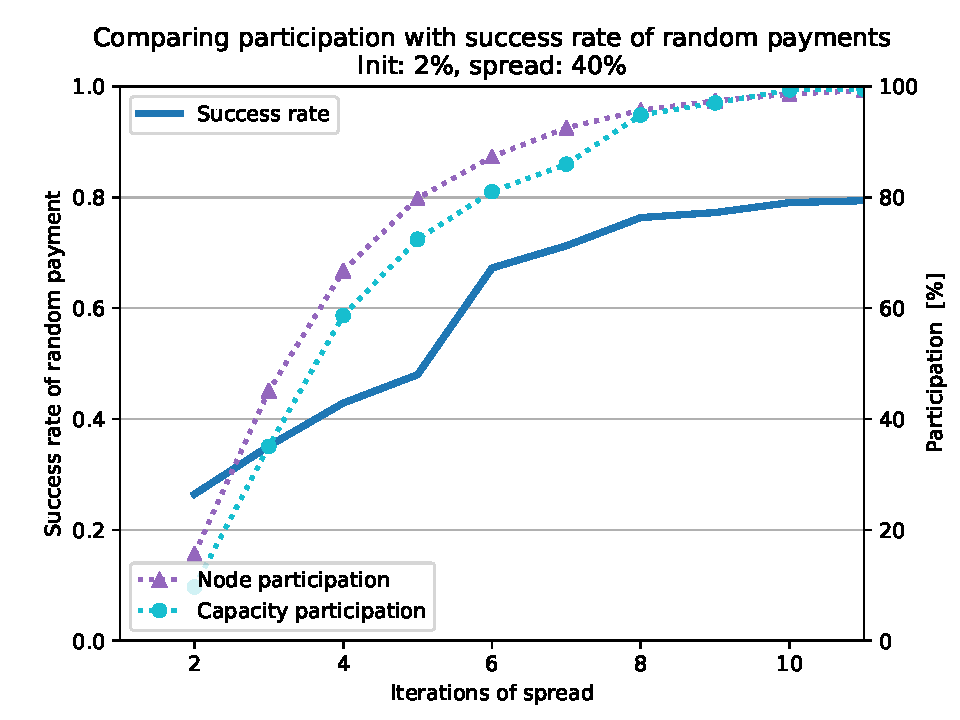
\includegraphics[width=60mm]{results/3a65a961_successrate_vs_participation_netw_spread_02_40.pdf} &   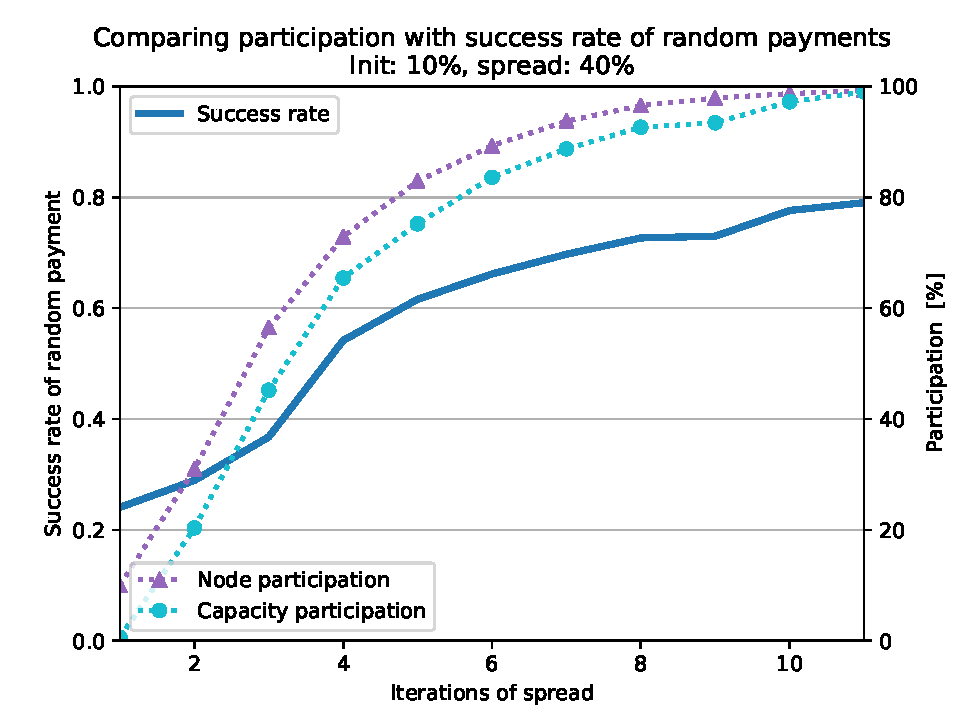
\includegraphics[width=60mm]{results/3a65a961_successrate_vs_participation_netw_spread_10_40.pdf} & 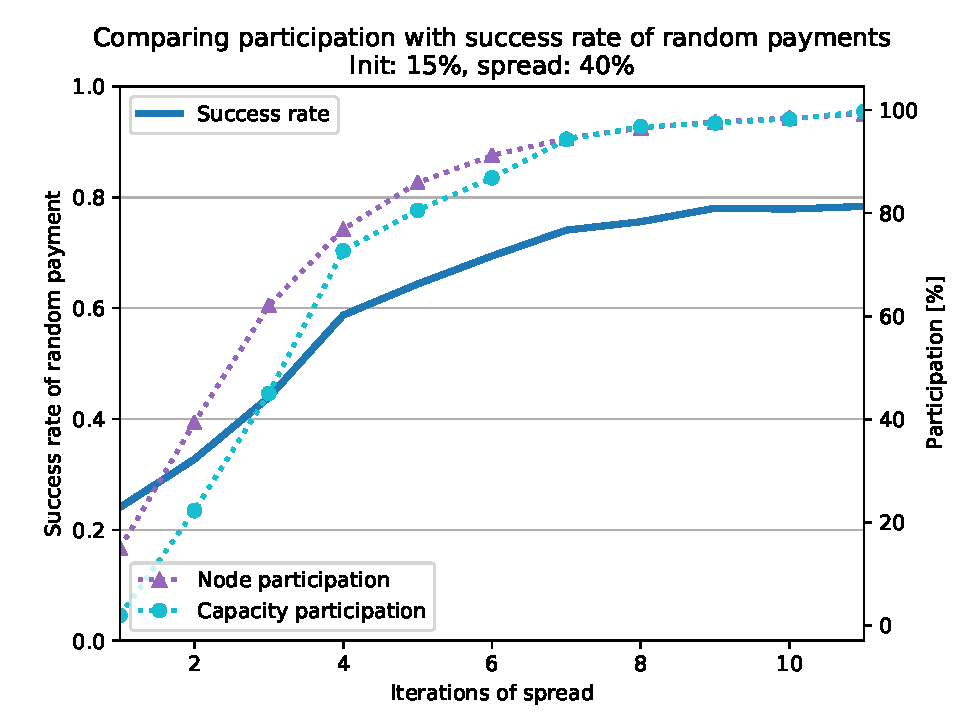
\includegraphics[width=60mm]{results/3a65a961_successrate_vs_participation_netw_spread_15_40.pdf}  \\
  (a) Init: 2 Spread: 40  & (b) Init: 10 Spread: 40 & (c) Init: 15 Spread: 40  \\[6pt]
  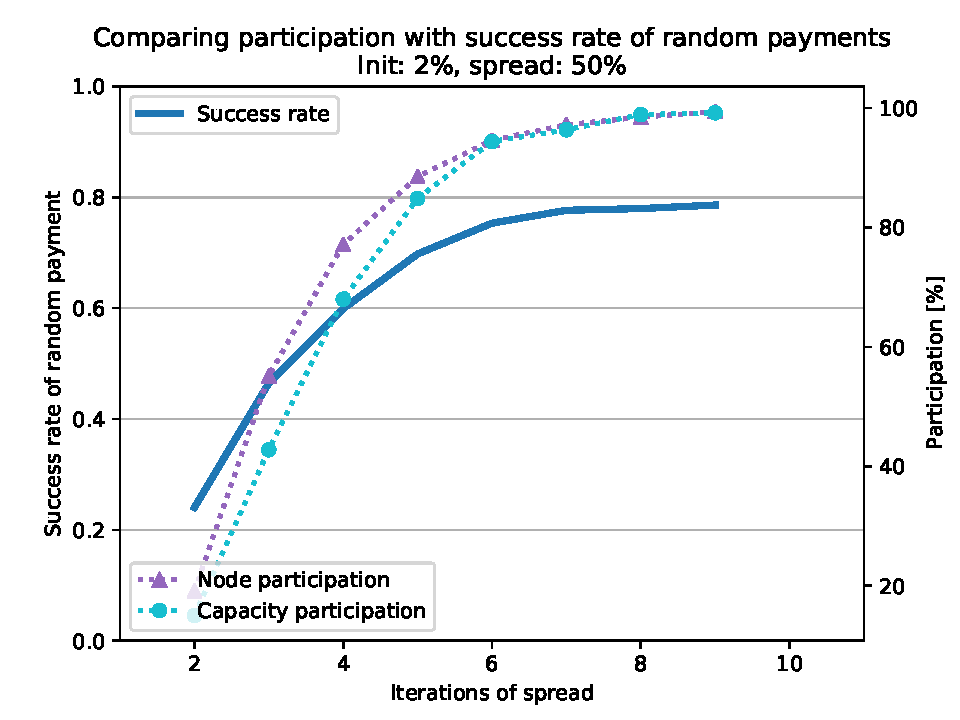
\includegraphics[width=60mm]{results/3a65a961_successrate_vs_participation_netw_spread_02_50.pdf} &   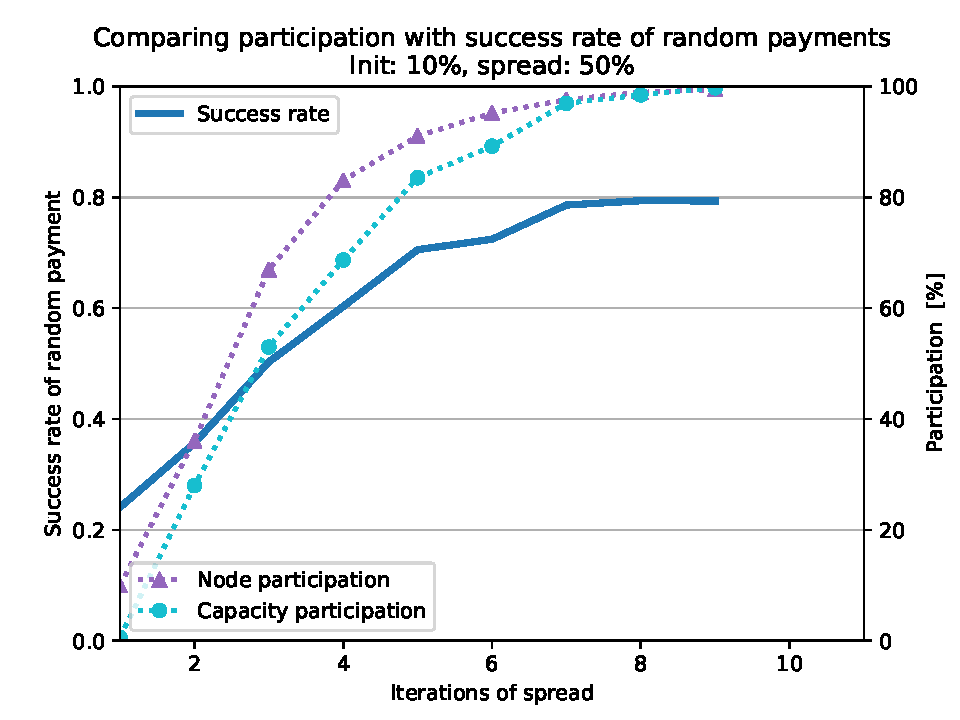
\includegraphics[width=60mm]{results/3a65a961_successrate_vs_participation_netw_spread_10_50.pdf} & 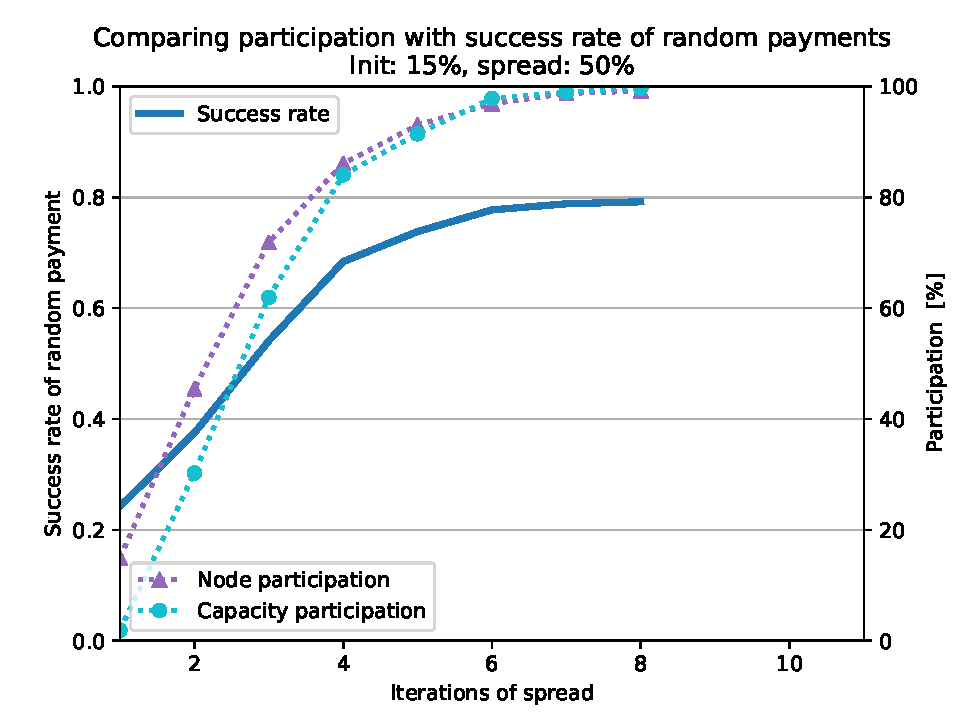
\includegraphics[width=60mm]{results/3a65a961_successrate_vs_participation_netw_spread_15_50.pdf}  \\
  (d) Init: 2 Spread: 50  & (e) Init: 10 Spread: 50 & (f) Init: 15 Spread: 50  \\[6pt]
  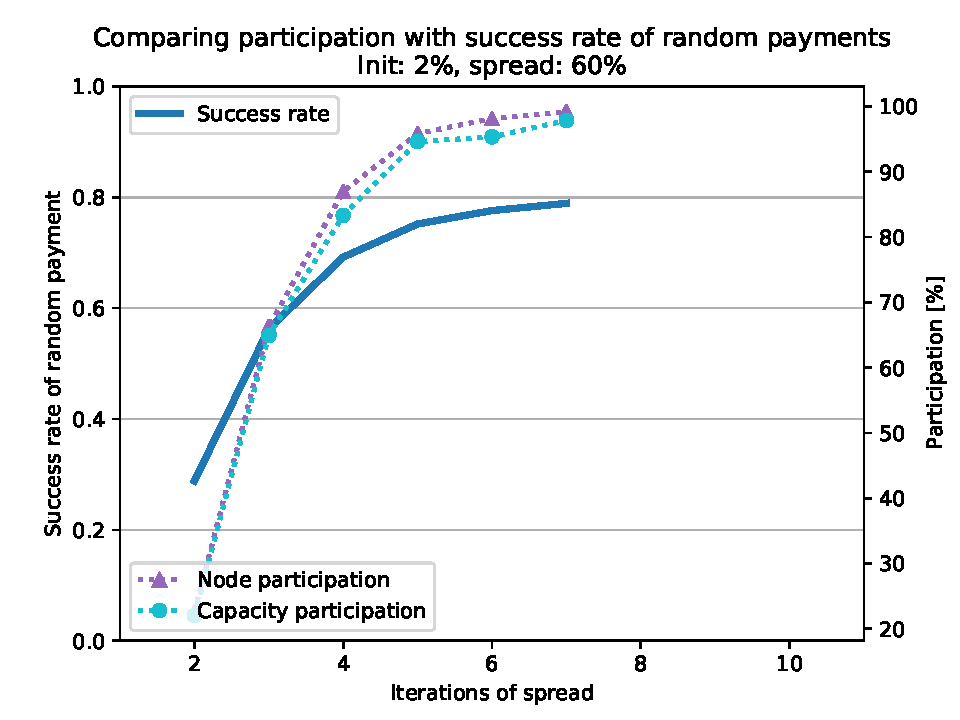
\includegraphics[width=60mm]{results/3a65a961_successrate_vs_participation_netw_spread_02_60.pdf} &   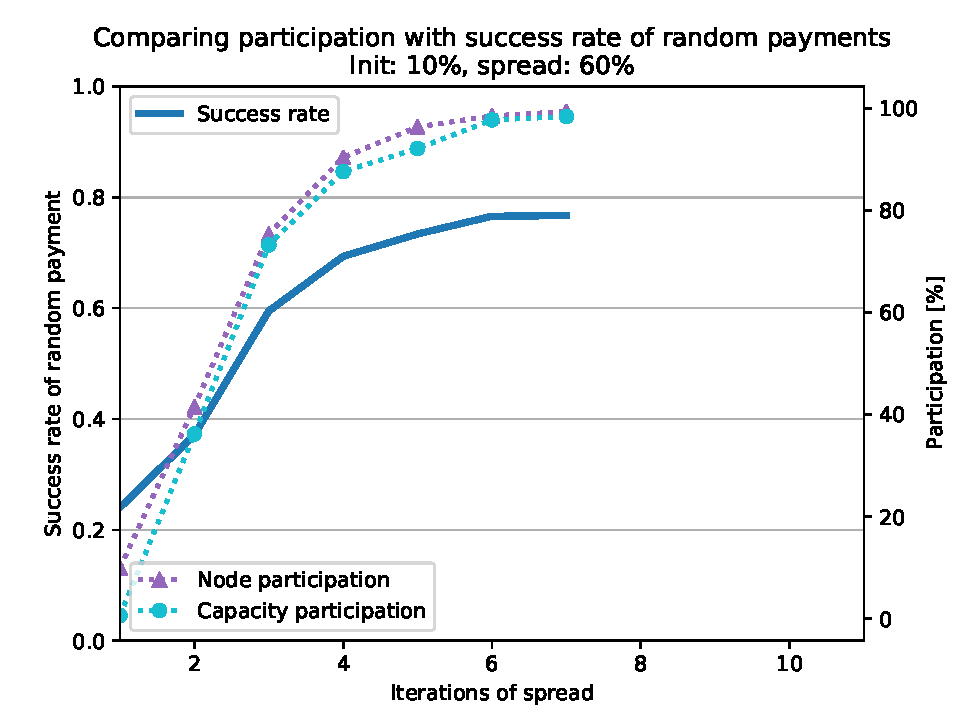
\includegraphics[width=60mm]{results/3a65a961_successrate_vs_participation_netw_spread_10_60.pdf} & 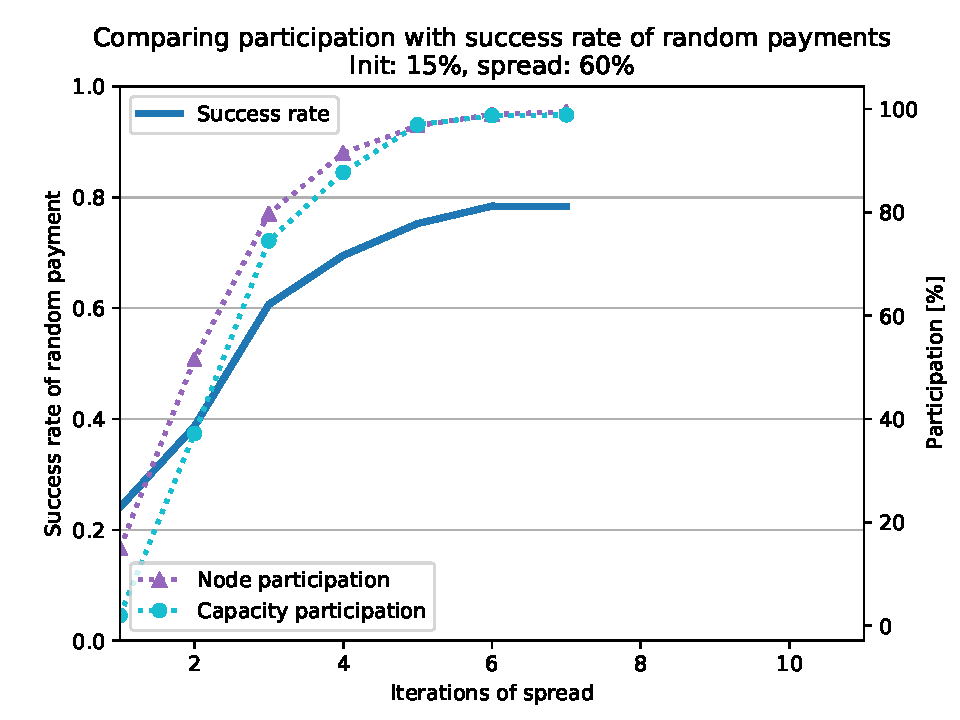
\includegraphics[width=60mm]{results/3a65a961_successrate_vs_participation_netw_spread_15_60.pdf}  \\
  (g) Init: 2 Spread: 60  & (h) Init: 10 Spread: 60 & (i) Init: 15 Spread: 60  \\[6pt]
\end{tabular}
\caption{\gls{sr} All Parametrisations of Network Spread}
\label{fig:sr_all_spread}
\end{figure}

\newpage 
\begin{figure}
\begin{tabular}{ccc}
  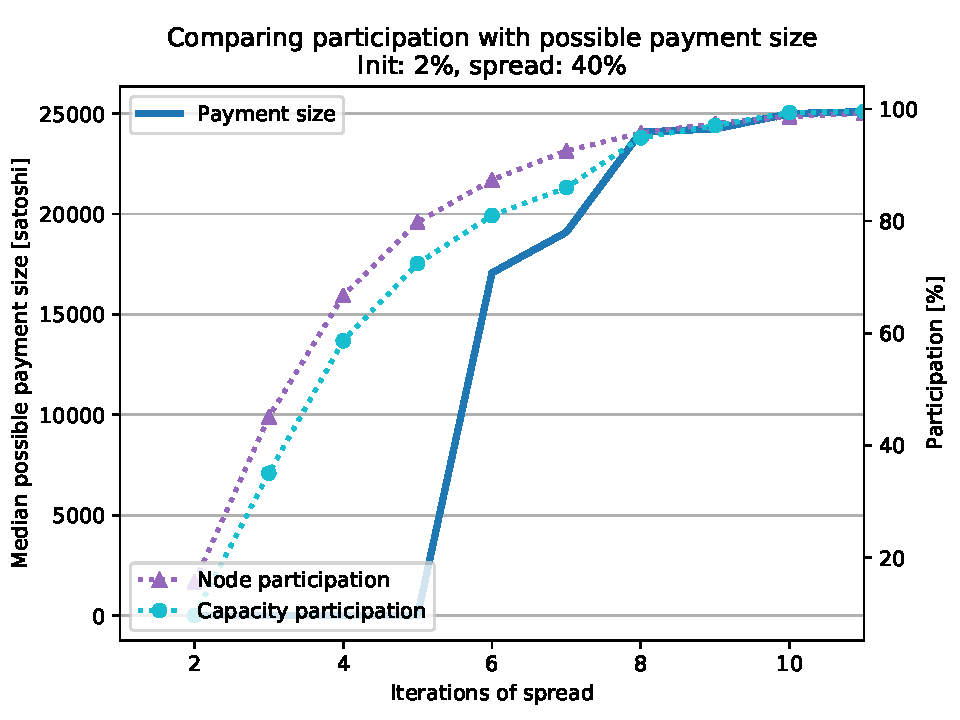
\includegraphics[width=60mm]{results/3a65a961_median_paymnet_size_vs_participation_netw_spread_02_40.pdf} &   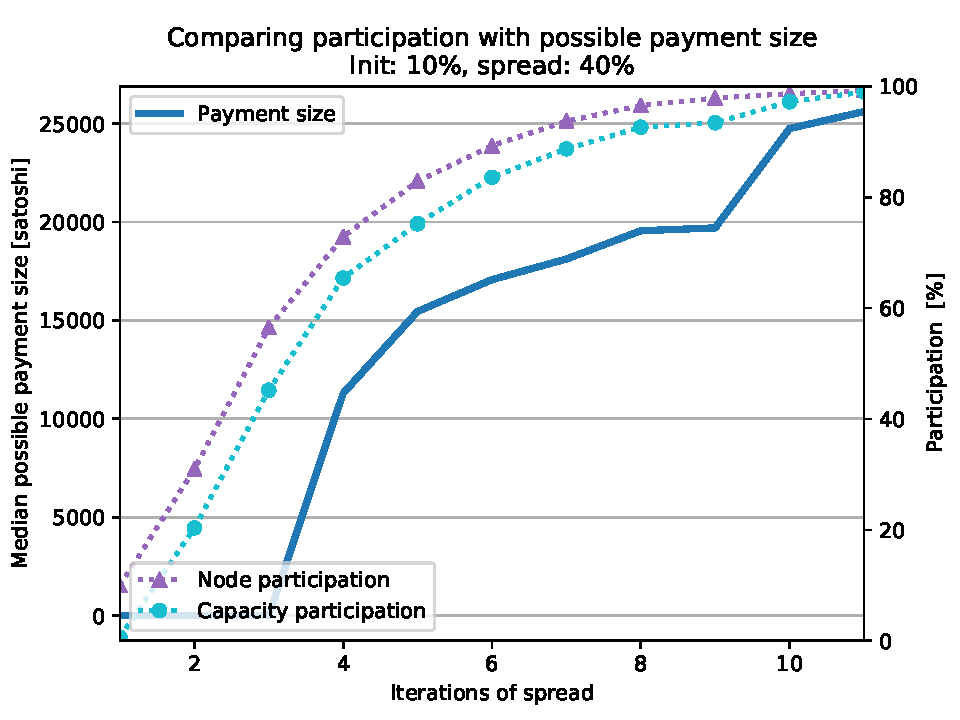
\includegraphics[width=60mm]{results/3a65a961_median_paymnet_size_vs_participation_netw_spread_10_40.pdf} & \includegraphics[width=60mm]{results/3a65a961_median_paymnet_size_vs_participation_netw_spread_15_40.pdf}  \\
  (a) Init: 2 Spread: 40  & (b) Init: 10 Spread: 40 & (c) Init: 15 Spread: 40  \\[6pt]
  \includegraphics[width=60mm]{results/3a65a961_median_paymnet_size_vs_participation_netw_spread_02_50.pdf} &   \includegraphics[width=60mm]{results/3a65a961_median_paymnet_size_vs_participation_netw_spread_10_50.pdf} & \includegraphics[width=60mm]{results/3a65a961_median_paymnet_size_vs_participation_netw_spread_15_50.pdf}  \\
  (d) Init: 2 Spread: 50  & (e) Init: 10 Spread: 50 & (f) Init: 15 Spread: 50  \\[6pt]
  \includegraphics[width=60mm]{results/3a65a961_median_paymnet_size_vs_participation_netw_spread_02_60.pdf} &   \includegraphics[width=60mm]{results/3a65a961_median_paymnet_size_vs_participation_netw_spread_10_60.pdf} & \includegraphics[width=60mm]{results/3a65a961_median_paymnet_size_vs_participation_netw_spread_15_60.pdf}  \\
  (g) Init: 2 Spread: 60  & (h) Init: 10 Spread: 60 & (i) Init: 15 Spread: 60  \\[6pt]
\end{tabular}
\caption{\gls{mps} All Parametrisations of Network Spread}
\label{fig:mps_all_spread}
\end{figure}

\newpage 
\begin{figure}
\begin{tabular}{ccc}
  \includegraphics[width=60mm]{results/3a65a961_median_paymnets_vs_participation_netw_spread_02_40.pdf} &   \includegraphics[width=60mm]{results/3a65a961_median_paymnets_vs_participation_netw_spread_10_40.pdf} & \includegraphics[width=60mm]{results/3a65a961_median_paymnets_vs_participation_netw_spread_15_40.pdf}  \\
  (a) Init: 2 Spread: 40  & (b) Init: 10 Spread: 40 & (c) Init: 15 Spread: 40  \\[6pt]
  \includegraphics[width=60mm]{results/3a65a961_median_paymnets_vs_participation_netw_spread_02_50.pdf} &   \includegraphics[width=60mm]{results/3a65a961_median_paymnets_vs_participation_netw_spread_10_50.pdf} & \includegraphics[width=60mm]{results/3a65a961_median_paymnets_vs_participation_netw_spread_15_50.pdf}  \\
  (d) Init: 2 Spread: 50  & (e) Init: 10 Spread: 50 & (f) Init: 15 Spread: 50  \\[6pt]
  \includegraphics[width=60mm]{results/3a65a961_median_paymnets_vs_participation_netw_spread_02_60.pdf} &   \includegraphics[width=60mm]{results/3a65a961_median_paymnets_vs_participation_netw_spread_10_60.pdf} & \includegraphics[width=60mm]{results/3a65a961_median_paymnets_vs_participation_netw_spread_15_60.pdf}  \\
  (g) Init: 2 Spread: 60  & (h) Init: 10 Spread: 60 & (i) Init: 15 Spread: 60  \\[6pt]
\end{tabular}
\caption{\gls{mpr} All Parametrisations of Network Spread}
\label{fig:mpr_all_spread}
\end{figure}

\newpage 
\begin{figure}
\begin{tabular}{ccc}
  \includegraphics[width=60mm]{results/3a65a961_gini_vs_participation_netw_spread_02_40.pdf} &   \includegraphics[width=60mm]{results/3a65a961_gini_vs_participation_netw_spread_10_40.pdf} & \includegraphics[width=60mm]{results/3a65a961_gini_vs_participation_netw_spread_15_40.pdf}  \\
  (a) Init: 2 Spread: 40  & (b) Init: 10 Spread: 40 & (c) Init: 15 Spread: 40  \\[6pt]
  \includegraphics[width=60mm]{results/3a65a961_gini_vs_participation_netw_spread_02_50.pdf} &   \includegraphics[width=60mm]{results/3a65a961_gini_vs_participation_netw_spread_10_50.pdf} & \includegraphics[width=60mm]{results/3a65a961_gini_vs_participation_netw_spread_15_50.pdf}  \\
  (d) Init: 2 Spread: 50  & (e) Init: 10 Spread: 50 & (f) Init: 15 Spread: 50  \\[6pt]
  \includegraphics[width=60mm]{results/3a65a961_gini_vs_participation_netw_spread_02_60.pdf} &   \includegraphics[width=60mm]{results/3a65a961_gini_vs_participation_netw_spread_10_60.pdf} & \includegraphics[width=60mm]{results/3a65a961_gini_vs_participation_netw_spread_15_60.pdf}  \\
  (g) Init: 2 Spread: 60  & (h) Init: 10 Spread: 60 & (i) Init: 15 Spread: 60  \\[6pt]
\end{tabular}
\caption{\gls{gini} All Parametrisations of Network Spread}
\label{fig:gini_all_spread}
\end{figure}
\restoregeometry

%%---TODO-OVERVIEW-------------------
\ifdraft{%Do this only if mode=draft
\newpage
\listoftodos[\section{Todo-Notes}]
\clearpage
}
{%Do this only if mode=final
}

\end{document}

